\section{Chapter introduction}

This chapter presents results of coupled regional climate simulations run with the ICOLMDZOR LAM to study the impacts of irrigation on land-atmosphere coupling variables and the water cycle over several years of simulation, with a focus on annual and seasonal means. 
The objective was to address the following questions:
\begin{itemize}
    \item Is simulated irrigation realistic in coupled simulations ? What are its limits and perspectives for improvements ?
    \item What impacts does simulated irrigation have on the water cycle and land-atmosphere interactions ? Does irrigation improve the ability of the model to represent them ?
    \item At the scale of the Iberian Peninsula, is the impact of irrigation limited to intensely irrigated areas or can remote effects be observed as a consequence of atmospheric feedbacks ?
    \item How are the impacts of irrigation modulated in a future climate, under a strong climate change scenario ?
\end{itemize}

%todo:check this abd update
This chapter first contains methodological aspects regarding the simulation setups used and the reference products used for evaluation of the LAM. 

Section \ref{sec:article1} then presents the impacts of irrigation on land-atmosphere interactions and the water cycle, under the present climate of the Iberian Peninsula. These results were presented in an article currently under review in Earth System Dynamics: \url{https://egusphere.copernicus.org/preprints/2025/egusphere-2025-2491/}.
The article was not included as a whole in this chapter but many elements were reused and adapted, to avoid redundancies with Chapters \ref{chap:introduction} and \ref{chap:methods} and enable a better integration with additional results from Sections \ref{chap:forcing} and \ref{sec:climate_change}, and Chapter \ref{chap:liaise}. The full article in its current version is available as an appendix to this manuscript.
Finally, Section \ref{sec:climate_change} presents preliminary results obtained from coupled simulations of future climate under a strong climate change scenario, highlighting the impacts of climate change over the Iberian Peninsula, and how they interact with irrigation.

%todo: evaluate need to metion this again 
% All the results presented in this chapter are derived from coupled simulation run with ICOLMDZ and ORCHIDEE using the LAM described in Chapter \ref{chap:methods}. The routing and irrigation schemes were used with the parameter set identified after the offline calibration presented in Chapter \ref{chap:routing}, and the MERIT DEM at 2-km resolution.

\clearpage

\section{Impacts of irrigation under present climate}
\label{sec:article1}
As mentionned in the chapter introduction, this section presents results and figures from an article currently under review in Earth System Dynamics and included as a whole in the appendix. %todo:internal ref

Two coupled simulations were run with the ICOLMDZOR LAM, using the intermediate domain size ($R_{domain}=1500km$ and $NBP=60$). The setups are identical except for the inclusion of irrigation, and are referred to as \irr (with irrigation activated in ORCHIDEE) and \noirr (without irrigation). 
They were run for 13 years from 2010 to 2022, which enables capturing some interannual variability of the current climate, making the averages less sensitive to anomalies or biases from any single year or extreme event.

\subsection{Simulated irrigation}
\label{sec:irrig_eval}

%figure
\begin{figure}[htbp]
    \centering
    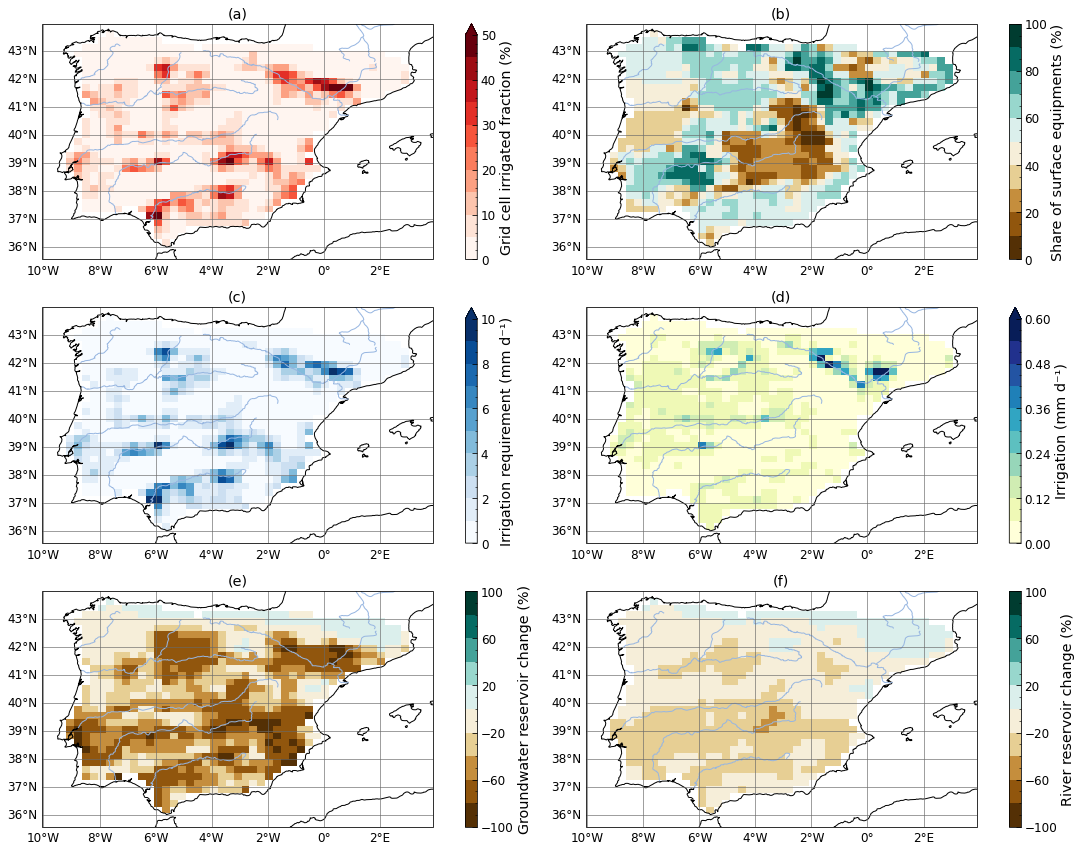
\includegraphics[width=\textwidth]{images/chap4/article/f03.png}
    \caption{Simulated irrigation and its drivers. Input maps of (a) grid cell irrigated fraction \citep[\% , derived from][]{hurtt_harmonization_2020} and (b) the share of irrigation equipment for surface withdrawals, as opposed to groundwater withdrawals \citep[\%, derived from ][]{siebert_groundwater_2010}. Annual means (2010-2022) of (c) simulated irrigation requirement (mm d$^{-1}$), (d) irrigation (mm d$^{-1}$), and relative changes (\irr - \noirr, \%) in water volumes in (e) groundwater and (f) river reservoirs.}
    \label{fig:irrig_maps}
\end{figure}

The computed irrigation demand (Fig. \ref{fig:irrig_maps}c) is highly dependent on the irrigated fraction (Fig. \ref{fig:irrig_maps}a) and much greater than the applied irrigation (Fig. \ref{fig:irrig_maps}d). This shows that irrigation is often constrained by water availability, with clear regional differences. Indeed, irrigation is much greater in the northern regions (Ebro and Douro river basins) than in southern regions (Guadiana and Guadalquivir basins) even though these regions have similar levels of irrigation demand (Fig. \ref{fig:irrig_maps}c, d).
As shown in Fig. \ref{fig:irrig_maps}b, southern regions (Guadalquivir Basin, upper Guadiana Basin) are more dependent on groundwater equipment for irrigation water withdrawals than the Ebro Basin, where withdrawals are taken mainly from surface water (overland and river reservoirs in the model).
Considering that the groundwater reservoir is much more depleted in the presence of irrigation than the river reservoir is (Fig. \ref{fig:irrig_maps}e, f), it is not surprising that the irrigation requirement cannot be met in these regions as much as it is in the north.
This depletion can be explained by the fact that the groundwater reservoir can only be filled with drainage in the grid cell, whereas the river reservoir can be fed from upstream grid cells and benefit from remote precipitation at the basin scale. It is also important to note that ORCHIDEE does not model deep groundwater storage, which is an important source of water for irrigation in southeastern Spain \citep{custodio_groundwater_2016}.

%figure : map of bias (irr vs obsEbro) + Seasonnal cycle over area with obs
\begin{figure}[htbp]
    \centering
    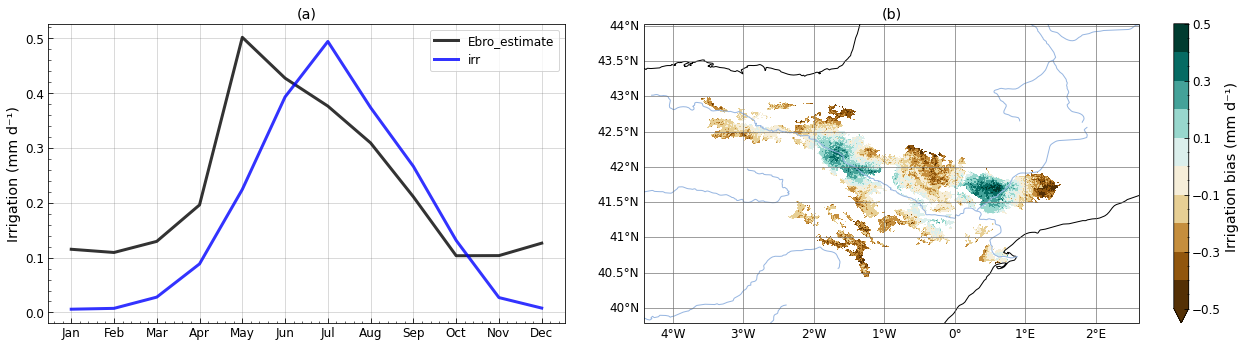
\includegraphics[width=\textwidth]{images/chap4/article/f04_horizontalized.png}
    \caption{Evaluation of simulated irrigation from January 2016 to July 2020 over the Ebro Valley. (a) Mean seasonal cycle of irrigation for the \irr simulation and the remote sensing product (\textit{Ebro\_estimate}, mm d$^{-1}$), and (b) mean bias compared with the product (mm d$^{-1}$). The simulation outputs are interpolated on the grid of the remote sensing product.}
    \label{fig:irrig_eval}
\end{figure}

In the Ebro Basin, simulated irrigation was evaluated using the irrigation remote sensing product from \cite{dari_regional_2023} with good overall performance, particularly in summer (Fig. \ref{fig:irrig_eval}a).
In winter, the model simulates almost no irrigation since it requires a minimum LAI to be activated, whereas the product shows irrigation all year long, which can be explained by the presence of winter crops not represented in the model.
A delay of the summer peak in the model compared with the product is noticeable, but the model might not be very far from actual irrigation since this product was found to be slightly ahead of actual irrigation based on benchmark volumes in some districts of the Ebro Valley \citep[Fig. 5 in ][]{dari_regional_2023}.
Spatially, the remote sensing product shows greater irrigation on the hillslopes than in the thalwegs, whereas the model simulates the opposite, with more intense irrigation next to the large rivers (Ebro, Segre, Cinca).
The resulting bias pattern (Fig. \ref{fig:irrig_eval}b) can be explained by the fact that in the model, water is mainly withdrawn from the river reservoir in this region, which is much greater in grid cells holding a large river than in upper areas of the valley. In reality, infrastructures such as the Canal d'Urgell in the Segre basin \citep{farran_urgell_2024}, enable gravity irrigation of hillslopes by diverting water from large rivers to neighbouring croplands. Including a representation of water adduction in the irrigation scheme by enabling withdrawal from adjacent grid cells could be a way to improve this bias.
Overall, the spatial biases of the simulated irrigation offset each other relatively well. Averaged over the subdomain where the satellite product provides values, the simulated irrigation is 0.20 mm d$^{-1}$ while the product estimates it at 0.23 mm d$^{-1}$.

\subsection{Impacts of irrigation on river discharge}
%todo:check que l'ajout des stations reste propre et cohérent

The simulated river discharge was evaluated against monthly data from 18 stations of the GRDC datbase (described in Section \ref{sec:eval_datasets}).
These stations, selected since they provided data over the simulation period and an had adequate position on the DEM grid, are described in Table \ref{table:stations_data} and shown in Fig. \ref{fig:selected_stations}. Most stations have available data from January 2010 to September 2017, and river discharge was therefore evaluated using the first eight years of simulation (2010-2017).

%figure:discharge stations and dams
\begin{figure}[htbp]
    \centering
    \includegraphics[width=\textwidth]{images/chap4/article/f02.pdf}
    \caption{Stations used for river discharge evaluation, river dams from \citet{aquastat_dams}, and main rivers of the study area from the CCM2.1 dataset \citep{vogt_pan-european_2007}, showing only rivers longer than 50 km for readability.}
    \label{fig:selected_stations}
\end{figure}

%table:description of discharge station used
\begin{table*}[htbp]
    \caption{Characteristics of river discharge stations used for evaluation. Stations marked with * are the largest of the five major basins of the Peninsula, and are shown in Fig. \ref{fig:discharge_SC}.
    }
    \resizebox{\textwidth}{!}{%
    \begin{tabular}{lcccccc}
        \toprule
        % \textbf{Station} & \textbf{Altitude (m)} & \textbf{River} & \textbf{Area (km²)} & \textbf{Mean discharge (m³/s)} & \textbf{Coverage (2010-2017, \%)} \\
        \textbf{Station} & \textbf{Altitude (m)} & \textbf{River} & \textbf{Area} & \textbf{Mean discharge} & \textbf{Coverage} \\
         & & & (km²) &  (m³/s) &  (2010-2017, \%) \\
        \midrule
        *1 (Tortosa)            & 25    & Ebro      & 84230     & 287.61 & 96.9 \\
        2 (Zaragoza)            & 189   & Ebro      & 40434     & 210.89 & 96.9 \\
        3 (Castejon)            & 265   & Ebro      & 25194     & 201.34 & 96.9 \\
        4 (Seros)               & 85    & Segre     & 12782     & 52.75  & 96.9 \\
        5 (Fraga)               & 100   & Cinca     & 9612      & 49.69  & 93.8 \\
        *6 (Tore)               & 637   & Douro     & 41808     & 109.18 & 96.9 \\
        7 (Peral De Arlanza)    & 766   & Arlanza   & 2413      & 16.44  & 96.9\\
        *8 (Talavera)           & 366   & Tagus     & 33849     & 46.77  & 34.4\\
        9 (Trillo)              & 727   & Tagus     & 3253      & 12.70  & 96.9 \\
        10 (Peralejos)          & 1143  & Tagus     & 410       & 3.87   & 96.9 \\
        *11 (Azud de Badajoz)   & 166   & Guadiana  & 48530     & 81.83  & 83.3 \\
        12 (Pulo do Lobo)       & 28    & Guadiana  & 61884     & 25.23  & 58.3 \\
        13 (La Cubeta)          & 758   & Guadiana  & 856       & 3.37   & 92.7 \\
        14 (Villarubia)         & 628   & Guadiana  & 10319     & 0.82   & 66.7 \\
        15 (Quintanar)          & 694   & Giguela   & 995       & 0.71   & 55.2 \\
        *16 (Mengibar)          & 240   & Guadalquivir & 16166  & 30.25  & 75.0 \\
        17 (Arroyo Maria)       & 538   & Guadalquivir & 583    & 6.19   & 86.5 \\
        18 (Pinos Puente)       & 561   & Frailes   & 357       & 1.00   & 87.5 \\
        \bottomrule
    \end{tabular}
    }
    \label{table:stations_data}
\end{table*}

%%single column figure : discharge obs vs irr vs no_irr on 3 stations (3 large rivers with proper data)
\begin{figure}[htbp]
    \centering
    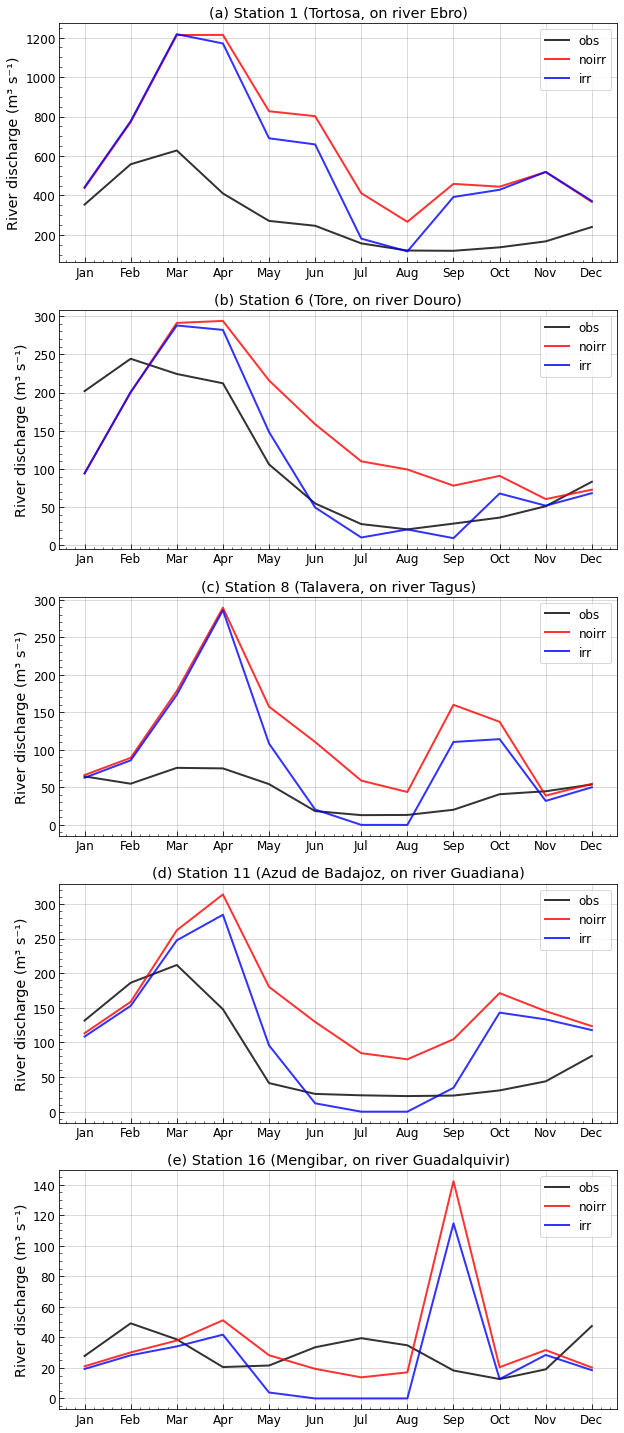
\includegraphics[width=8.3cm]{images/chap4/article/f05.png} 
    \caption{Impacts of irrigation on river discharge. Mean seasonal cycle of river discharge (m$^3$ s$^{-1}$) in observations (black) and the \noirr (red) and \irr (blue) simulations at five stations: (a) Tortosa (Ebro), (b) Tore (Douro), (c) Talavera (Tagus), (d) Azud de Badajoz (Guadiana), and (e) Mengibar (Guadalquivir). A mask is applied to the simulations to filter out months without corresponding observation data.}
    \label{fig:discharge_SC}
\end{figure}

Figure \ref{fig:discharge_SC} shows the average seasonal cycle of river discharge for the five largest rivers of the Peninsula (Ebro, Douro, Tagus, Guadiana, and Guadalquivir), for the two simulations and the GRDC observation data. The station with the greatest river discharge was selected for each river, to reflect integrated impacts of irrigation over the basin. A similar figure with all eighteen stations is presented in the appendix (Fig. \ref{fig:TS_discharge_18stations}, \ref{fig:TS_discharge_18stations}).
In most cases, the model shows a slight delay and a large overestimation of river discharge compared with observations, particularly in winter and spring. These errors can be related to the precipitation biases of the simulations, described in the next section, and to the lack of river dams in the model, which have a strong impact on actual discharge, given their high density in the Iberian Peninsula \citep[Fig. \ref{fig:selected_stations}, ][]{sabater_chapter_2022, moran-tejeda_reservoir_2012, lobera_geomorphic_2015}. In particular, the model overestimates the winter and spring discharge, a period when water is stored in dam reservoirs, which reduces the actual river flow.
The presence of dams also leads to unnatural seasonal cycles in the observations if river discharge is artificially increased in summer by the release of stored water (Fig. \ref{fig:discharge_SC}e).

The simulation of irrigation used cannot improve either of these aspects since it does not include a specific reservoir to store water. Its impact becomes noticeable in spring, with water withdrawals resulting in lower discharge during summer and autumn, generally leading to a much better match with observations (Fig. \ref{fig:discharge_SC}). 
As shown in Table \ref{table:stations_metrics}, for all fifteen stations where the mean bias is positive in the \noirr simulation, this bias is reduced in the presence of irrigation (in three cases it becomes negative but the absolute value is reduced). However, for the three stations where the \noirr bias is negative (n°10, 13, 17), it is worsened in the \irr simulation. On average, the \irr simulation exhibits clear improvements of the mean bias (-41.8 \%) and root mean square error (RMSE, -7.12 \%). The Pearson correlation coefficient is 0.56 on average in \noirr and is slightly improved (+0.02), with mostly small changes except for stations 6 and 8 (+0.09 and +0.08). Improvements are also observed for Nash-Sutcliffe efficiency (NSE, +0.67) and Kling-Gupta efficiency (KGE, +0.2), mostly as a consequence of improvements in the mean bias. However, only eight out of eighteen stations have a positive value of NSE and KGE values in the \noirr simulation (not shown), limiting the relevance of this average increase. In particular, the average NSE value is strongly influenced by a few stations (n°5, 8, 15) with initial NSE values below -10.

Overall, the performance is clearly improved for 12 stations but partly degraded for 6 stations, although three of them (n°10, 13, 17) have a very small average discharge. This may explain why small changes in the model can lead to large changes in performance and limits their relevance compared with larger stations. If only stations with an average annual discharge greater than 10 m³ s$^{-1}$ are considered, irrigation improves performance in nine out of twelve cases, and degrades it for three stations. One station (n°9) exhibits an unexpected increase in the spring discharge peak which originates mostly from a single year (2011, see Fig. \ref{fig:TS_discharge_18stations}) and worsens an already-existing 250 \% bias in this season. The other two (n°4 and 5) are close to the Pyrenees mountains and present very strong biases in both simulations (300 \% overestimation in spring, unexpected double peak in March and June, Fig. A2). These discrepancies are likely related to biases in precipitation (discussed hereafter) and were not positively impacted by irrigation, apart from the mean bias.

\begin{table*}[hbtp]
    \resizebox{\textwidth}{!}{
    \begin{tabular}{lccccccccc}
        \toprule
        \textbf{Station} & \textbf{Mean discharge} & \textbf{Bias} & \textbf{Bias} & \textbf{RMSE change} & \textbf{r change} & \textbf{NSE change} & \textbf{KGE change} \\
        & (\textit{obs}, m$^3$ s$^{-1}$) & (\noirr,  \%) & (\irr, \%)  & (\textit{irr - no\_irr}, \%) & (\textit{irr - no\_irr}) & (\textit{irr - no\_irr})  & (\textit{irr - no\_irr})  \\
        % \textbf{Station} & \textbf{Mean discharge (obs, m³/s)} & \textbf{Bias\\(\noirr, \%)} & \textbf{Bias\\Change (\%)} & \textbf{RMSE\\Change (\%)} & \textbf{r\\change} & \textbf{NSE\\change} & \textbf{KGE\\change} \\

        \midrule
        *1 (Tortosa)        & 287.61  & 126.3 & \textbf{103.4} & \textbf{-7.88} & \textbf{0.03}  & \textbf{0.56}  & \textbf{0.13}  \\
        2 (Zaragoza)        & 210.89  & 27.6 & \textbf{11.5}   & \textbf{-13.10}  & \textbf{0.01}  & \textbf{0.06}  & \textbf{0.10}  \\
        3 (Castejon)        & 201.34  & 30.7 & \textbf{21.4}   & \textbf{-1.45}  & \textbf{0.01}  & \textbf{0.01}  & \textbf{0.03}  \\
        4 (Seros)           & 52.75   & 240.3 & \textbf{227.7} & 0.81   & -0.02 & -0.54 & -0.09 \\
        5 (Fraga)           & 49.69   & 193.2 & \textbf{179.8} & 1.81   & -0.01 & -1.78 & -0.22 \\
        *6 (Tore)           & 109.18  & 36.9 & \textbf{-0.2}   & \textbf{-16.24} & \textbf{0.09}  & \textbf{0.21}  & \textbf{0.25}  \\
        7 (Peral De Arlanza) & 16.44  & 40.7 & \textbf{35.2}   & \textbf{-3.12}  & \textbf{0.01}  & \textbf{0.04}  & \textbf{0.04}  \\
        *8 (Talavera)       & 46.77   & 152.4 & \textbf{95.8}  & \textbf{-10.84} & \textbf{0.08}  & \textbf{2.29}  & \textbf{0.16}  \\
        9 (Trillo)          & 12.70   & 60.8 & \textbf{59.7}   & 0.76   & \textbf{0.03}  & -0.15 & -0.05 \\
        10 (Peralejos)      & 3.87    & -34.6 & -38            & 1.82   & \textbf{0.01}  & -0.03 & -0.01 \\
        *11 (Azud de Badajoz) & 81.83 & 90.5 & \textbf{34.3}   & \textbf{-14.26} & \textbf{0.05}  & \textbf{0.24}  & \textbf{0.51}  \\
        12 (Pulo do Lobo)   & 25.23   & 287.3 & \textbf{162.0} & \textbf{-18.53} & \textbf{0.03}  & \textbf{1.48}  & \textbf{1.17}  \\
        13 (La Cubeta)      & 3.37    & -10.7 & -36.2          & 5.82   & -0.01 & -0.12 & -0.12 \\
        14 (Villarubia)     & 0.82    & 152.4 & \textbf{61.0}  & \textbf{-3.53} & -0.03 & \textbf{0.29}  & \textbf{0.53}  \\
        15 (Quintanar)      & 0.71    & 312.7 & \textbf{149.3} & \textbf{-17.89} & 0.00  & \textbf{9.31}  & \textbf{0.98}  \\
        *16 (Mengibar)      & 30.25   & 19.4 & \textbf{-16.9}  & \textbf{-4.52} & \textbf{0.01}  & \textbf{0.46}  & \textbf{0.09}  \\
        17 (Arroyo Maria)   & 6.19    & -35.4 & -47.5 & 8.44   & -0.04 & -0.28 & -0.10 \\
        18 (Pinos Puente)   & 1.00    & 27.0 & \textbf{-3.0}   & \textbf{-5.59}  & \textbf{0.03}  & \textbf{0.06}  & \textbf{0.12}  \\
        \midrule
        Mean                & 63.37   & 95.4 & \textbf{55.5}   & \textbf{-7.12} & \textbf{0.02}  & \textbf{0.67}  & \textbf{0.20}  \\
        \bottomrule
    \end{tabular}
    }
    \caption{Station mean discharge (\textit{obs}, m$^3$ s$^{-1}$), discharge bias (for the \noirr and \irr simulations, in \%), and change in evaluated metrics (\irr - \noirr) for the RMSE (relative change in \%), Pearson correlation coefficient $r$, Nash-Sutcliffe efficiency and Kling-Gupta efficiency \citep{gupta_decomposition_2009}. Model performance improvements when using irrigation are shown in bold. Stations marked with * are the largest of the five major basins of the Peninsula, and are shown in Fig. \ref{fig:discharge_SC}.}
    \label{table:stations_metrics}
\end{table*}

% \clearpage

\subsection{Evaluation of precipitation and ET and influence of irrigation}

%figure: precip and ET eval, side by side Seasonal Cycle (with obs products) and bias to GPCC/GLEAM
\begin{figure}[htbp]
    \centering
    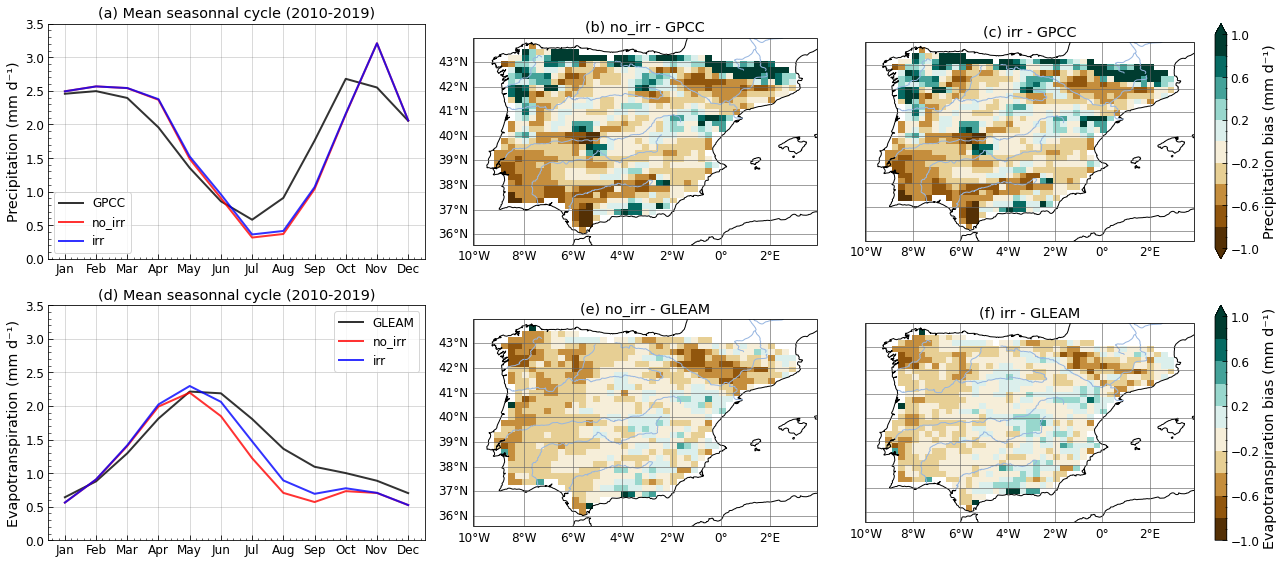
\includegraphics[width=\textwidth]{images/chap4/article/f06.png}
    \caption{Evaluation of simulated precipitation (P) and evapotranspiration (ET) over the Iberian Peninsula continental subdomain, from 2010 to 2019. 
    (a) Mean seasonal cycle of P (mm d$^{-1}$) for the two simulations and GPCC product, annual mean P bias of the (b) \noirr and (c) \irr simulations relative to the GPCC product (mm d$^{-1}$).
    (d) Mean seasonal cycle of ET (mm d$^{-1}$) for the two simulations and GLEAM4 product, annual mean ET bias of the (e) \noirr and (f) \irr simulations relative to the GLEAM4 product (mm d$^{-1}$).}
    \label{fig:sim_eval_ET_P}
\end{figure}

The simulated precipitation and ET were evaluated from 2010 to 2019 using the GPCC and GLEAM4 products, respectively (Fig. \ref{fig:sim_eval_ET_P}).
On average over the domain, the two simulations present very similar seasonal cycles of precipitation. The model is in good agreement with GPCC until June (Fig. \ref{fig:sim_eval_ET_P}a), but presents a strong underestimation of precipitation in summer, followed by a delayed and overestimated peak in autumn, which likely contributes to the biases of river discharge winter peaks visible in Fig. \ref{fig:discharge_SC}. 
This seasonal cycle is largely representative of the whole peninsula, although some spatial disparities persist. The two simulations exhibit very similar spatial patterns of annual mean precipitation, with a strong overestimation in elevated areas (Fig. \ref{fig:sim_eval_ET_P}b,c), which is a known bias of climate models \citep{arjdal_modeling_2024, adhikari_evaluation_2024}.
This is partly compensated by smaller underestimates of precipitation over large neighbouring areas, as seen in the Ebro Valley.

Both simulations match the GLEAM4 ET product well from January to May but underestimate ET for the rest of the year, particularly in summer (Fig. \ref{fig:sim_eval_ET_P}d). As expected, ET increases when irrigation is accounted for, particularly from May to September, which is the period where vegetation is the most developed and irrigation is the greatest. This partially alleviates the dry bias, but ET remains underestimated, even in the \irr simulation.
No similar patterns of biases between ET and incoming radiative fluxes were identified, and the remaining ET bias can be related to the underestimation of precipitation in the southwestern part of the Peninsula and in plains, such as the northern Ebro Valley (Fig. \ref{fig:sim_eval_ET_P}b, e). 
Along large rivers, the ET underestimation almost disappears in the \irr simulation (Fig. \ref{fig:sim_eval_ET_P}f). The increase in soil moisture due to irrigation directly translates into an increase in ET, corroborating the hypothesis that the region lies within the transition regime described by \citet{Budyko_1956}. 
In contrast, the ET bias remains significant in lightly irrigated grid cells such as hillslopes, which is consistent with the limits of simulated irrigation described in Section \ref{sec:irrig_eval} (Fig. \ref{fig:irrig_eval}).

\subsection{Atmospheric impacts of irrigation in summer}
\label{sec:jja_atmospheric_impacts}
\subsubsection{Statistical significance}
To assess the influence of irrigation on the model, a statistical significance test was used to filter out differences between the two simulations (\irr and \noirr) that may be the result of natural variability only. In Fig. \ref{fig:diff_sig_6vars}, a Student t-test is used to assess for each grid cell whether the mean difference between the two simulations  (\irr - \noirr) significantly differs from 0, with a p-value of 0.05 as the limit to reject the null hypothesis. Grid cells with nonsignificant changes are partly hidden with hatches.

\subsubsection{Results}
%figure : maps of JJA diff with non-sig grid cells hatched 
\begin{figure}[htbp]
    \centering
    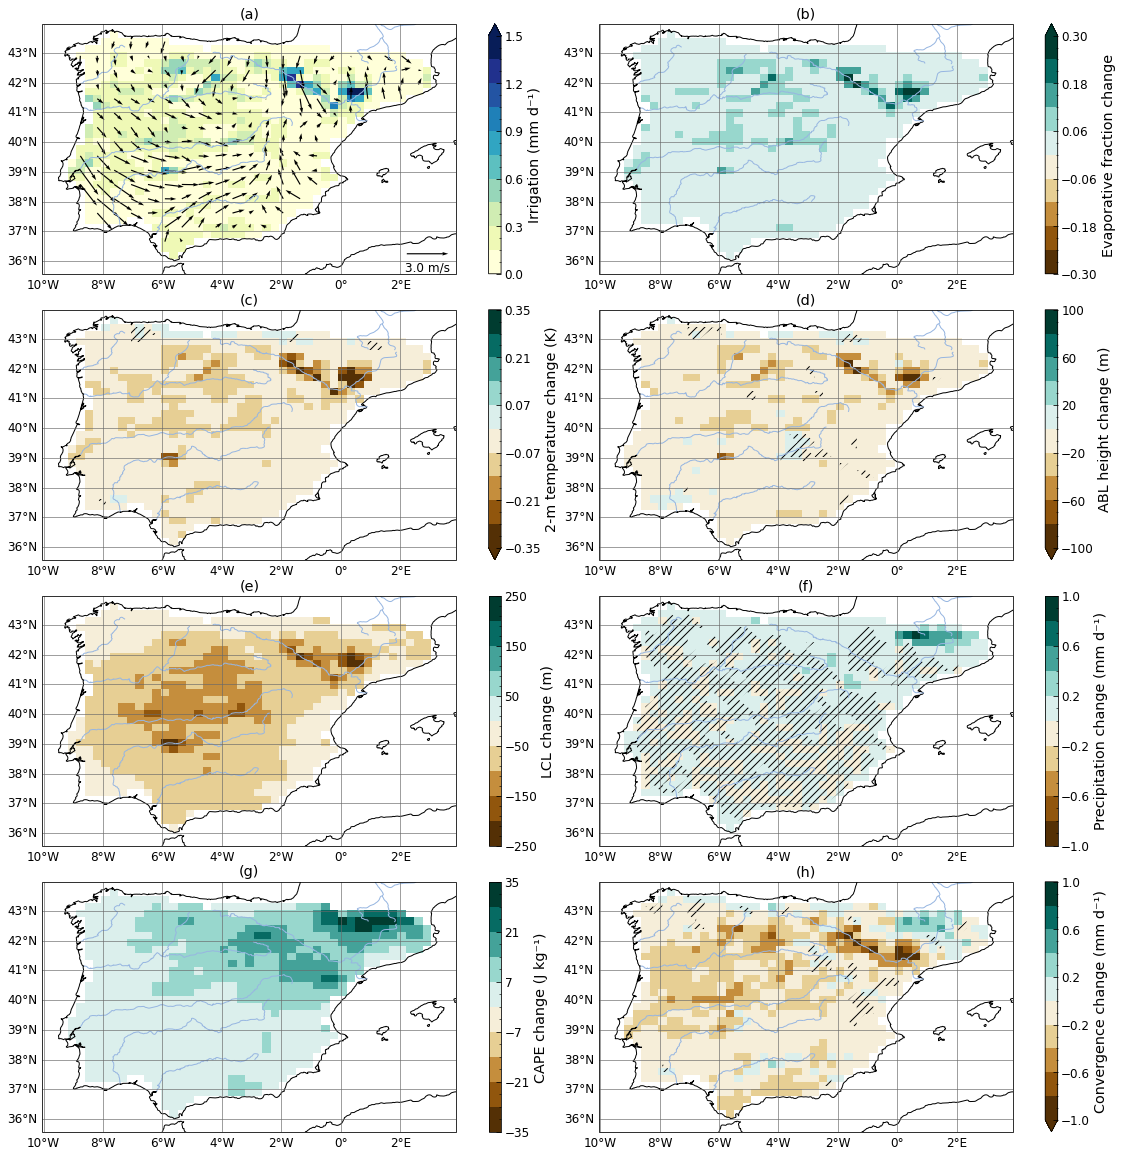
\includegraphics[width=15cm]{images/chap4/article/f07.png}
    \caption{Summer irrigation and its impacts (JJA, 2010-2022). (a) Irrigation (mm d$^{-1}$) and 10 m wind (\irr simulation). Mean changes in the presence of irrigation (\irr - \noirr): (b) evaporative fraction, (c) 2 m temperature (K), (d) atmospheric boundary layer height (m), (e) lifting condensation level (m), (f) precipitation (mm d$^{-1}$), (g) convective available potential energy (J kg$^{-1}$), (h) moisture convergence (mm d$^{-1}$). Hatching indicates areas where the change is not statistically significant.}
    \label{fig:diff_sig_6vars}
\end{figure}

The impacts of irrigation on atmospheric variables were studied with a focus on summer (JJA) since it is the season with the highest levels of simulated irrigation, with seasonal mean values of up to 1.5 mm d$^{-1}$ in the most intensely irrigated grid cells (Fig. \ref{fig:diff_sig_6vars}a).
In the presence of irrigation, the simulated latent heat flux ($LE$) increases across the entire Iberian Peninsula, by up to 50 W m$^{-2}$ in the Ebro Valley. As expected from the surface energy partitioning, this is compensated by a decrease in the sensible heat flux ($H$), which is almost equivalent in irrigated areas and leads to large increases in the evaporative fraction ($EF = \frac{LE}{LE+H}$) shown in Fig. \ref{fig:diff_sig_6vars}b.
When the sensible heat flux decreases, less energy is transmitted from the surface to the air, leading to a decrease in the 2-m air temperature which spatially matches the increase in $EF$. The order of magnitude remains low over most of the Peninsula, with the most important changes reaching -0.35 K in the Ebro Valley (Fig. \ref{fig:diff_sig_6vars}c).
The decreases in sensible heat flux and temperature also lead to a more stable boundary layer over most of the peninsula, but mostly in intensely irrigated areas where it is lowered by 100m (Fig. \ref{fig:diff_sig_6vars}d).
Moreover, the presence of irrigation results in a moister lower atmosphere, with an average specific humidity over the Peninsula increasing by 2.8 10$^{-4}$ kg kg$^{-1}$ in summer (+3.4 \%) and maximal local increases in the Ebro Valley of 1 10$^{-3}$ kg kg$^{-1}$ (+10 \%). Since air temperature changes in the atmospheric column are rather small, the lowering of the lifting condensation level (LCL) reflects this atmospheric moistening very well. It is most marked in the Ebro Valley, where the LCL is lowered by 250 m (-13 \%) in the most intensely irrigated grid cells, and remains significant even in areas where irrigation is low (Fig. \ref{fig:diff_sig_6vars}e).

The lowering of the ABL and LCL theoretically favour opposite effects on precipitation. On the one hand,  a lower and more stable ABL inhibits vertical mixing and convection, reducing the likelihood of cloud formation and deep convection initiation. On the other hand, if the LCL is lower, air parcels do not need to be lifted as high to condense, which increases the likelihood of cloud formation.
Over the most intensely irrigated areas, ABL stabilization seems to dominate and inhibit convective development since no significant change in precipitation is observed.
However, mountainous areas surrounding the Ebro Valley show significant increases in precipitation (Fig. \ref{fig:diff_sig_6vars}f). This can be understood because ABL stabilization remains weak in these zones whereas humidity can still be increased if moisture is advected (Fig. \ref{fig:diff_sig_6vars}d, e). In particular, the dominant wind patterns in the Ebro Valley (Fig. \ref{fig:diff_sig_6vars}a) indicate that the additional atmospheric moisture from irrigated areas is driven towards the valley slopes, which is consistent with the increases in moisture convergence (Fig. \ref{fig:diff_sig_6vars}h) and precipitation over the Pyrenees.
The competing interactions of ABL stabilization and atmospheric moistening are reflected by the increases in convective available potential energy (CAPE) which are most important in elevated areas around the valley (Fig. \ref{fig:diff_sig_6vars}g), where increases in precipitation are significant. 

% \clearpage

\subsection{Atmospheric moisture recycling over the Iberian Peninsula}
\label{sec:recycling}
On average over the continental domain, the monthly change in ET in the presence of irrigation is well correlated with the amount of water added by irrigation and even exceeds it, particularly in summer months (the orange JJA data points in Fig. \ref{fig:scatter_IP}a are all on or above the 1:1 line).
In the simulation, ET is constrained by available water, and almost all the water added by irrigation is evaporated or transpired, meaning that this additional increase in ET comes from an additional input of water into the soil.
This is explained by a systematic increase in precipitation over the domain (all the data points are on or above the x-axis on Fig. \ref{fig:scatter_IP}b). This increase is also roughly proportional to the amount of applied irrigation, although the correlation is weaker than that for the increase in ET, and its values remain lower than the amount of water added by irrigation.
Therefore, it appears that irrigation contributes to an increase in atmospheric moisture, and that a part of this moisture is recycled as continental precipitation, which can then be reevaporated.

%figure: 2 scatter plots over IP domain, rainDiff vs irrig
\begin{figure}[htbp]
    \centering
    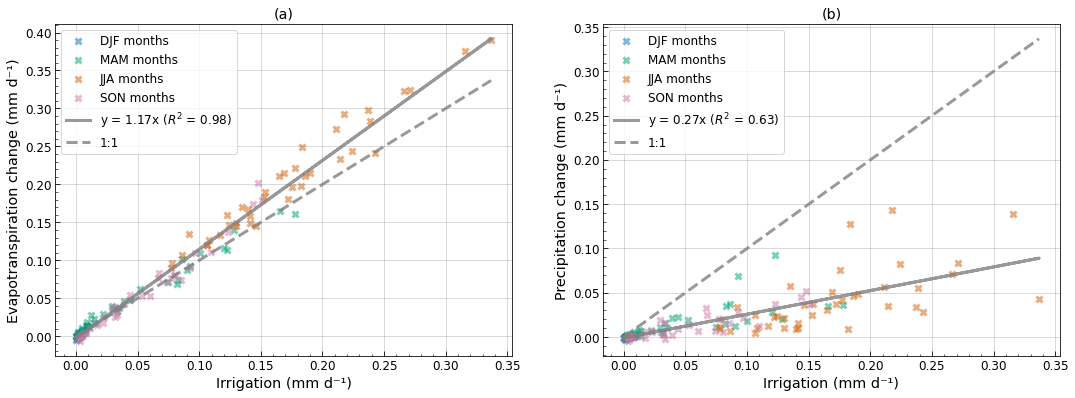
\includegraphics[width=\textwidth]{images/chap4/article/f08_colorblind.png}
    \caption{Domain-averaged influence of irrigation on monthly changes in ET and P (2010-2022). Each data point corresponds to the average value over the Iberian Peninsula continental domain for a single month of simulation (156 data points for 12 months over 13 years). The average amount of water added by irrigation in the \irr simulation (mm d$^{-1}$) is plotted against the average change (\textit{irr - no\_irr}) in (a) ET (mm d$^{-1}$) and (b) P (mm d$^{-1}$). The data points for the winter months are all concentrated around (0,0) for both figures because of very small irrigation volumes and changes in ET and P during this season.}
    \label{fig:scatter_IP}
\end{figure}

To look further into this recycling, three subdomains were defined, namely, low, medium and high irrigation areas, on the basis of the mean irrigation thresholds given in Table \ref{tab:irrig_lvl_areas}. In the map of simulated irrigation (Fig. \ref{fig:irrig_maps}d), the low irrigation domain corresponds to the first colour bin (yellow), the medium irrigation domain to the second bin (light green), and the high irrigation domain to the eight other bins. The three subdomains are also shown distinctly in Fig. \ref{fig:moisture_budget_annual}e.
On average, the increase in ET is slightly superior to irrigation for each subdomain (Fig. \ref{fig:moisture_budget_annual}).
However, the increase in precipitation is more than twice as large for the low irrigation subdomain than for the medium and high irrigation subdomains. Since irrigated areas are mostly in plains and valleys, this result is consistent with the increase in precipitation already described over mountainous areas in summer (Fig. \ref{fig:diff_sig_6vars}f). It points towards a nonlocal moisture recycling, with atmospheric moisture transfer from intensely irrigated areas to neighbouring lightly irrigated areas, meaning that a significant part of the additional rainfall does not occur on irrigated crops.
Over the entire Iberian Peninsula, the increase in precipitation represents 25 \% of the irrigated volume, whereas the increase in ET amounts to 112 \% of irrigation.

%t
% \begin{table}[t]
\begin{table}[h]
        \begin{tabular}{lcccc}
            \toprule
            \textbf{Subdomain} & \textbf{Areal fraction} & \textbf{Min. irrigation} & \textbf{Max. irrigation} & \textbf{Mean irrigation}\\
            & (\% of Iberian Peninsula) & (mm d$^{-1}$) & (mm d$^{-1}$) & (mm d$^{-1}$)\\
            \midrule
            Low irrigation      & 56.3    & 0.0   & 0.06  & 0.033 \\
            \midrule
            Medium irrigation   &  34.0   & 0.06  & 0.12  & 0.082\\
            \midrule
            High irrigation     &  9.7   & 0.12  & 0.61  & 0.210\\
            \bottomrule
        \end{tabular}
    \label{tab:irrig_lvl_areas}
    \caption{Subdomains of different irrigation intensity.}
\end{table}

%figure: moisture budget : barplot for 3 zones +IP
\begin{figure}[htbp]
    \centering
    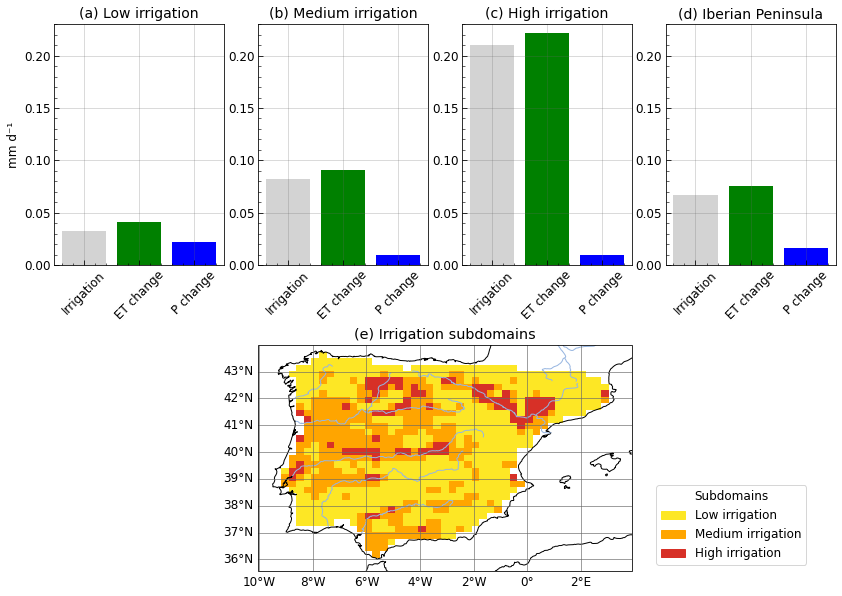
\includegraphics[width=12cm]{images/chap4/article/f09.png}
    \caption{Changes in the atmospheric moisture budget for subdomains with different irrigation intensities. Each bar plot shows the annual mean irrigation in the \irr simulation (2010-2022, mm d$^{-1}$) alongside the changes (\textit{irr - no\_irr}) in ET (mm d$^{-1}$) and P (mm d$^{-1}$) averaged over distinct subsets of the domain: (a) low irrigation, grid cells with an annual average irrigation lower than 0.06 mm d$^{-1}$, (b) medium irrigation, those where it is between 0.06 and 0.12 mm d$^{-1}$, (c) high irrigation those where it is higher than 0.12 mm d$^{-1}$, and (d) the Iberian Peninsula includes all 3 subsets. The three subdomains are shown in (e).}
    \label{fig:moisture_budget_annual}
\end{figure}

\clearpage

\clearpage

\section{Future climate of the Iberian Peninsula and impacts of irrigation under climate change}
\label{sec:climate_change}
This section is based on the results of Mariame Maiga's internship for her 1st year of Masters at Sorbonne Université, which I co-supervised with Frédérique Cheruy from April to July 2025. The impact of climate change was studied during the internship but not the effects of irrigation in the future, which was analysed later. All simulations used in this section were run by Frédérique Cheruy. 
Multiple technical issues were encountered to obtain reliable simulations of future climate with and without irrigation, therefore these results remain preliminary.

\hfill

To simulate future climate conditions, the LAM is used with forcing data from a global ICOLMDZOR simulation, under climate change scenario SSP5-8.5, which presents the strongest increase in global mean temperature. The mid-century period 2050-2062 was studied and compared to the present period (2010-2022). Longer simulations are under analysis to extend the study period to 30 years for both present and future but they were not yet available when writing this manuscript.
The smaller LAM domain ($R_{domain} = 1000 km$, $NBP=40$) was used for computational efficiency, considering the findings of Section \ref{sec:forcing_influence} that the inconsistencies on the edges of the domain are limited when the LAM is forced by ICOLMDZOR.

Simulations without irrigation in the present (\presnoirr) and future climate (\futnoirr) are compared to characterize the impacts of climate change over the Peninsula. Then, \futnoirr is compared to a simulation over the same period, with irrigation (\futirr) to analyse how irrigation interacts with these impacts.

\subsection{Impact of climate change over the Iberian Peninsula}

The annual impact of climate change under the SSP5-8.5 scenario on land-atmosphere coupling variables is presented in Fig. \ref{fig:diffmaps_present_future}, as the difference between the \futnoirr (2050-2062) and \presnoirr (2010-2022) simulations. 
%temperature
A general warming of the air is observed, as expected with a strong climate change scenario, with 2-m temperature increases of 2°C in most of the domain and up to 3°C in the northern half of the Peninsula (Fig. \ref{fig:diffmaps_present_future}a). The coasts are slightly less affected by warming, whereas the moutain ranges are the most impacted regions.
%precip
Precipitation decreases over most of the Peninsula, especially in the northern coast and the Pyrenees while the only region where it increases is the Southeast (Fig. \ref{fig:diffmaps_present_future}c). This region usually receives little precipitation so, although the absolute values are small, the relative increase is higher than 10\% over a large area and exceeds 25\% in several grid cells (Fig. \ref{fig:reldiffmaps_present_future}).
%evap and fluxsens
The changes in precipitation translate into similar changes in ET, of lower magnitude (Fig. \ref{fig:diffmaps_present_future}d). The only exceptions are in  Pyrenees and Cantabrian mountain ranges in the North, which are very humid areas where ET is limited by incoming radiation rather than available soil moisture.
The sensible heat flux is increased over almost all the continental domain  (Fig. \ref{fig:diffmaps_present_future}b). This evolution is not only a consequence of changes in surface energy partitionning since increases are also visible in areas where ET is increasing. It is likely dominated by an increase in the incoming energy at the surface, since it closely linked to increases in downwelling shortwave radiation (Fig. \ref{fig:diffmaps_present_future}g).
%q2m and RH2m
Specific humidity at 2m is increased over all the domain, with the largest increases reaching $1 g \cdot kg^{-1}$ on coastal areas (Fig. \ref{fig:diffmaps_present_future}e), which corresponds to a 10\% increase. Considering the increase in 2-m air temperature, this can be understood using the Clausius-Clapeyron relation, showing that warmer air can contain more water. %option:quote IPCC WG1 box on precipitation
However, under climate change, the increase in specific humidity is not as impactful as the increase in temperature since relative humidity at 2m is lower over all the continental domain (Fig. \ref{fig:diffmaps_present_future}f), especially in the North of the Peninsula. 
%link to rad fluxes and cloud cover
This explains the increase in the downwelling shortwave radiation flux (Fig. \ref{fig:diffmaps_present_future}g) since less condensed water is present in the atmosphere, particularly in the Northwest of the Peninsula. 
The general increase in longwave downwelling radiation (Fig. \ref{fig:diffmaps_present_future}h) is the consequence of a warmer atmosphere, but this increase is not as large in the North and Northwest of the domain, which is consistent with a lower relative humidity and cloud cover over these regions. 
%option : cloud cover in Appendix ? (with low, medium, high ?)

%figure : diff maps (no_irr, present - future)
\begin{figure}[htbp]
    \centering
    \begin{tabular}{cc}
        %t2m
        \begin{subfigure}[b]{0.5\textwidth}
            \caption{2-m temperature difference}
            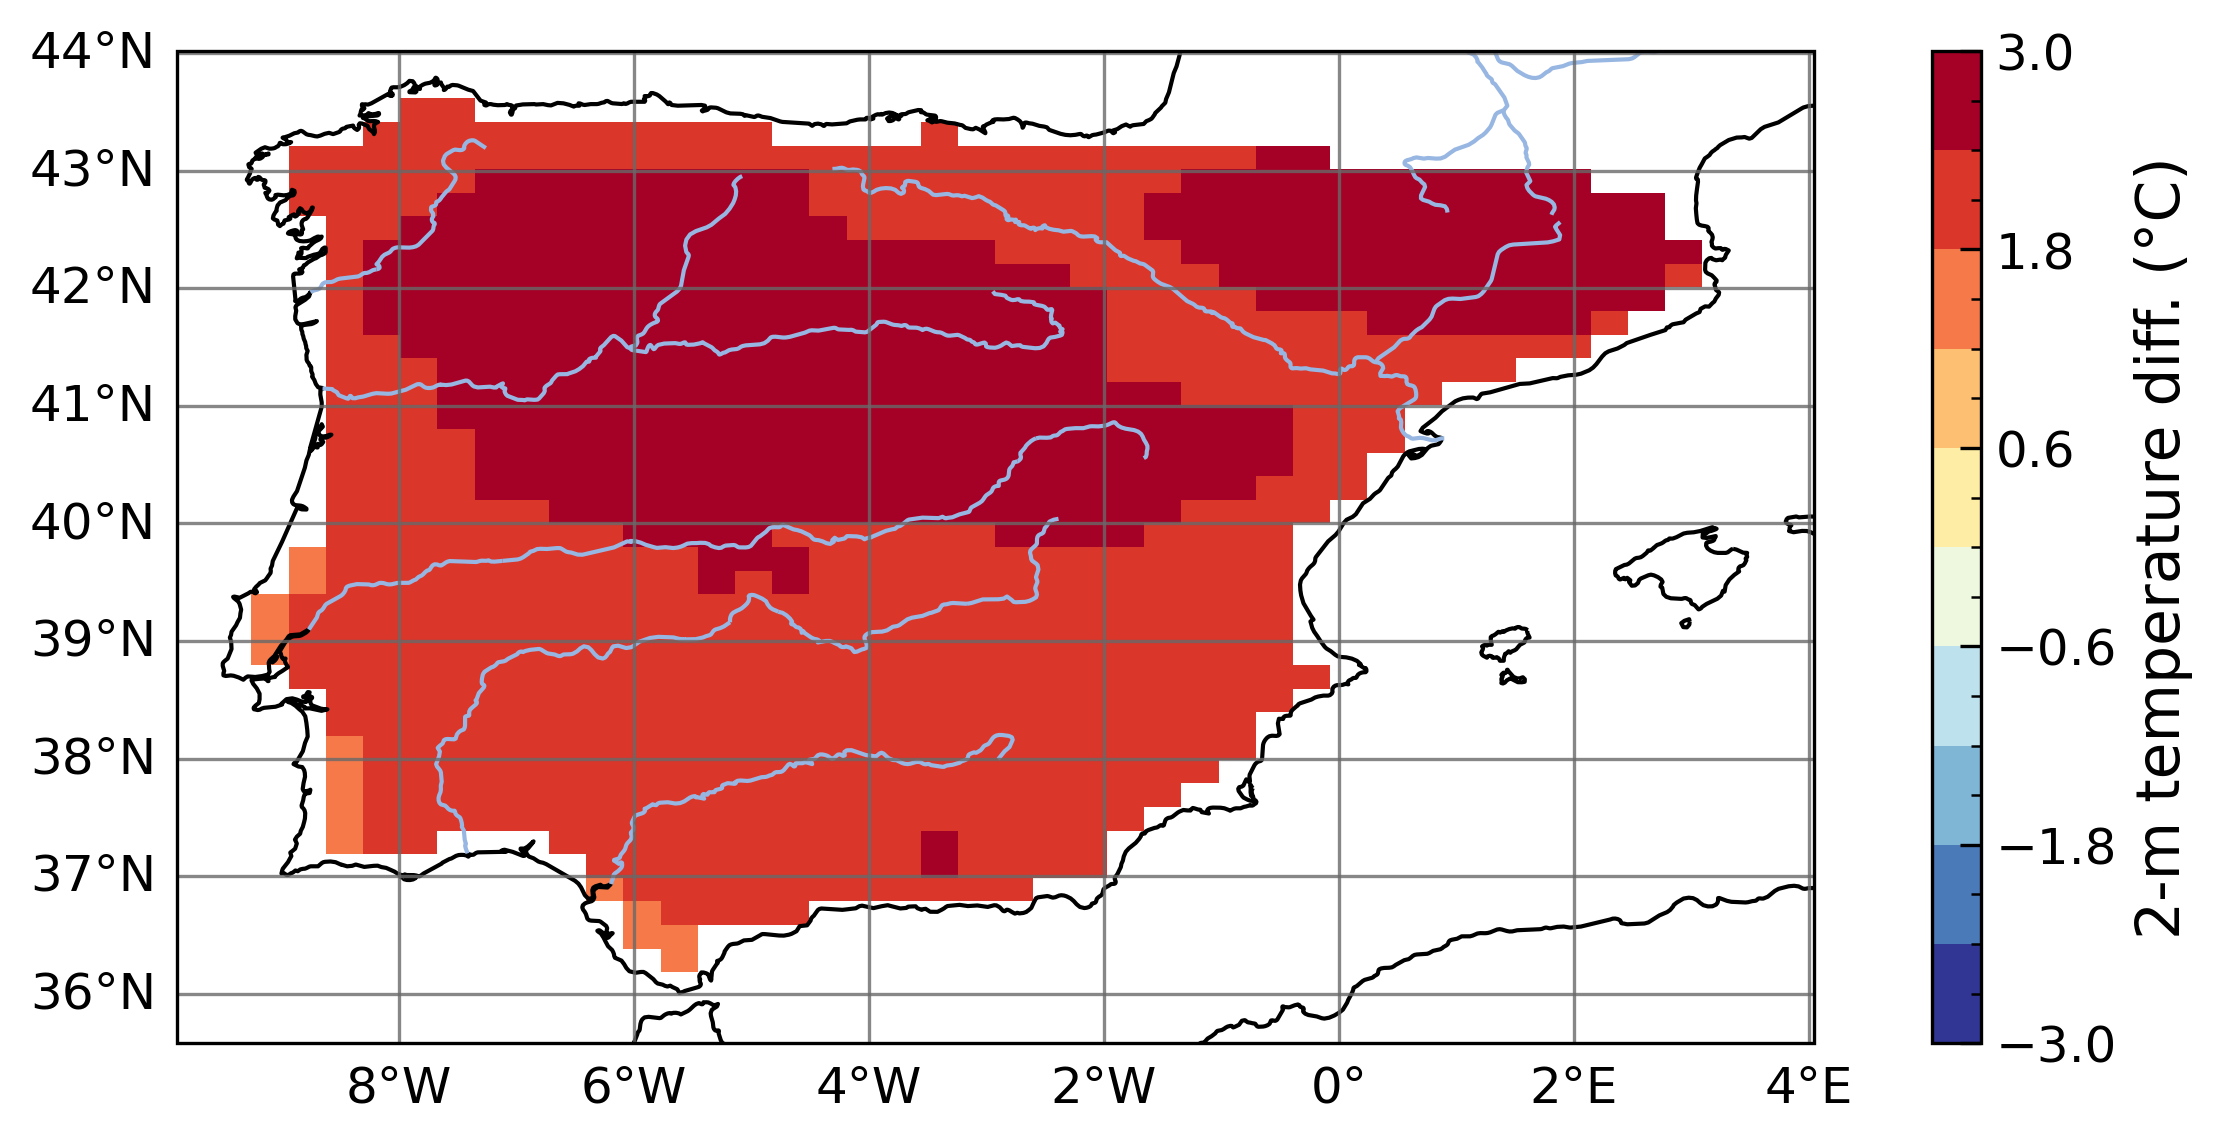
\includegraphics[width=\textwidth]{images/chap4/future/diffmap_t2m_presfut.png}
        \end{subfigure} &
        %fluxsens
        \begin{subfigure}[b]{0.5\textwidth}
            \caption{Sensible heat flux difference}
            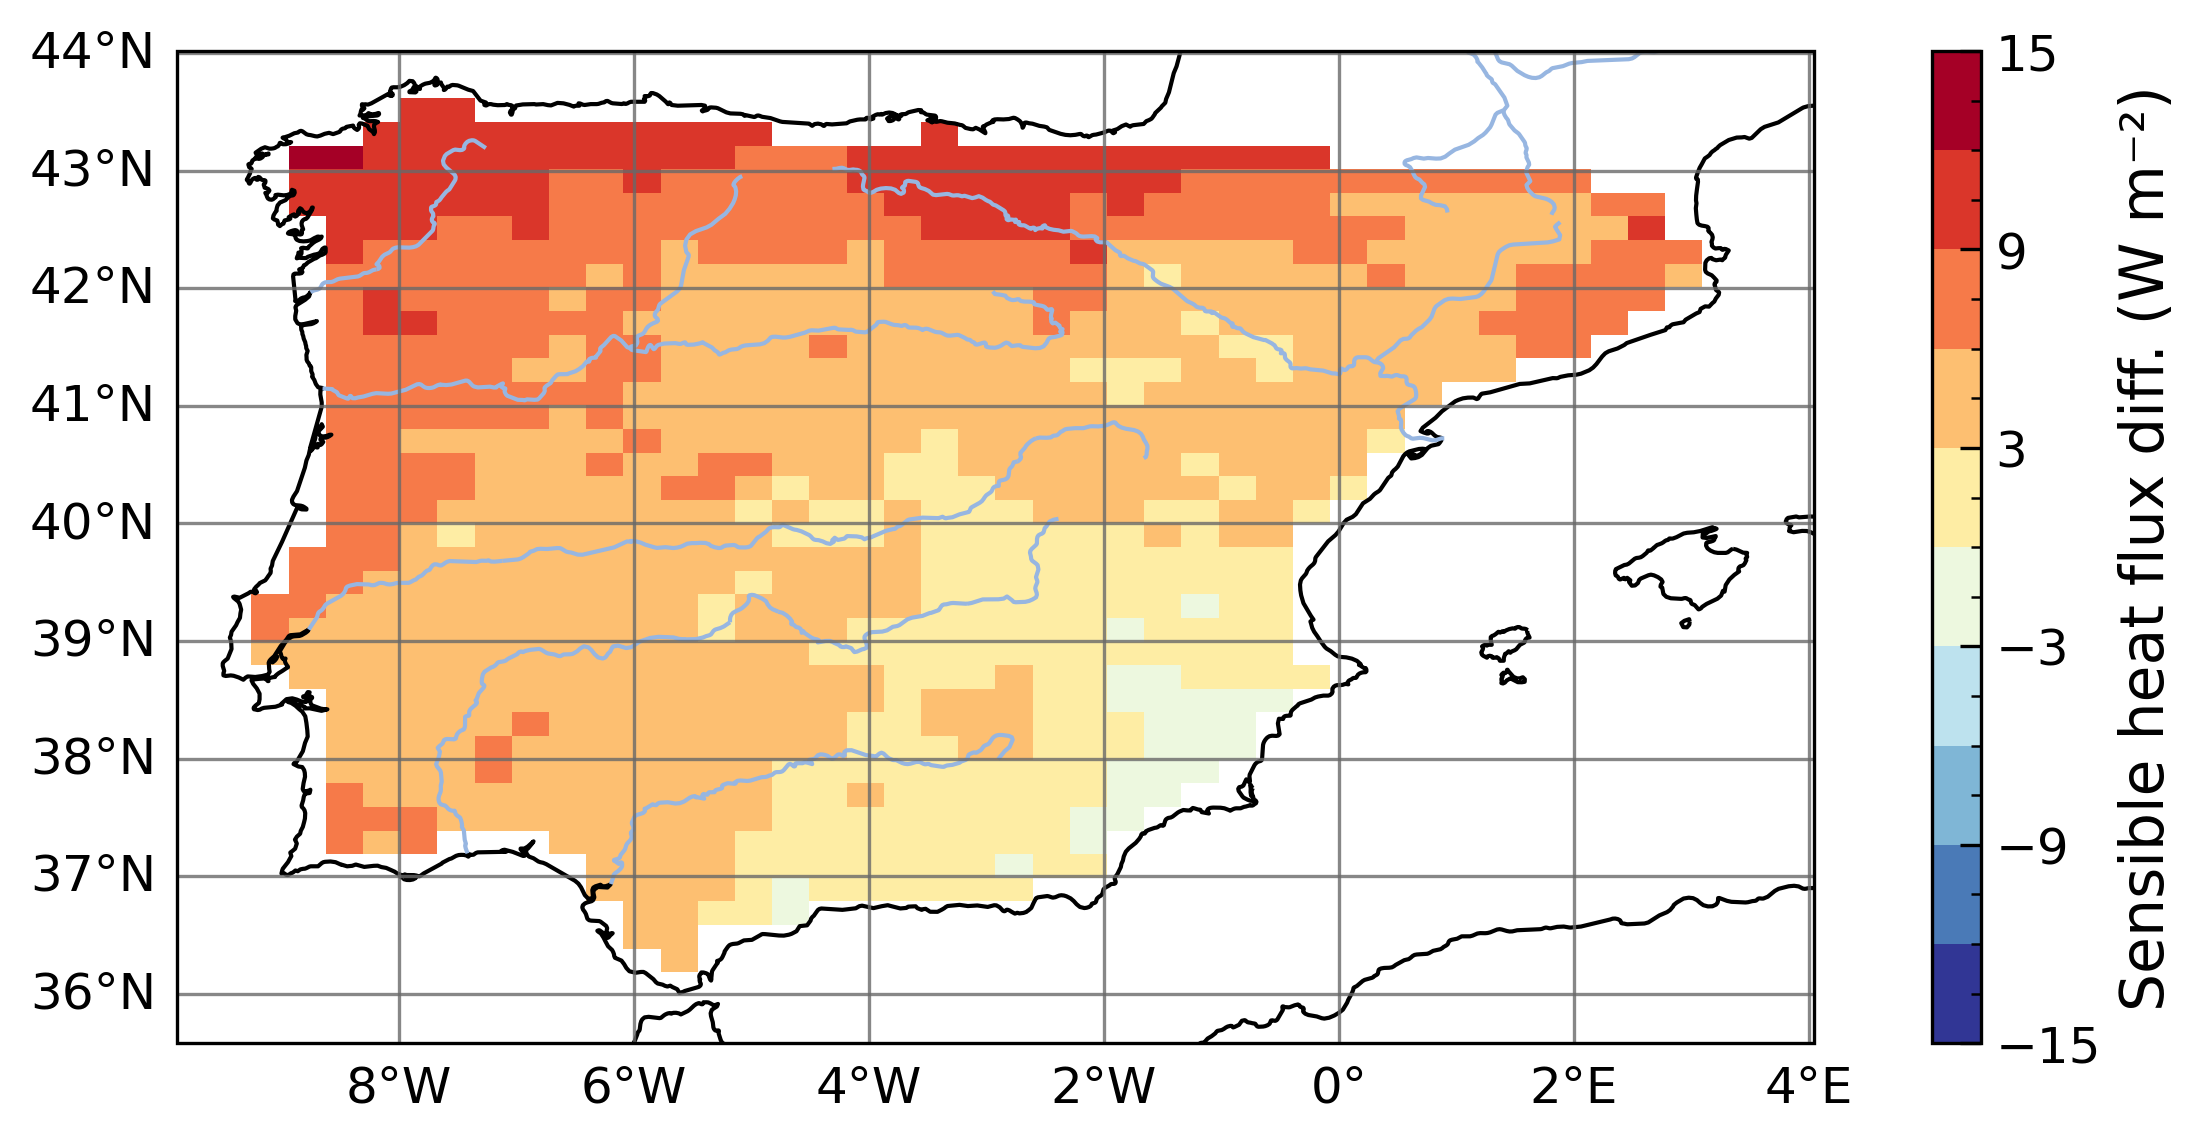
\includegraphics[width=\textwidth]{images/chap4/future/diffmap_fluxsens_presfut.png}
        \end{subfigure} \\
        
        %precip
        \begin{subfigure}[b]{0.5\textwidth}
            \caption{Precipitation difference}
            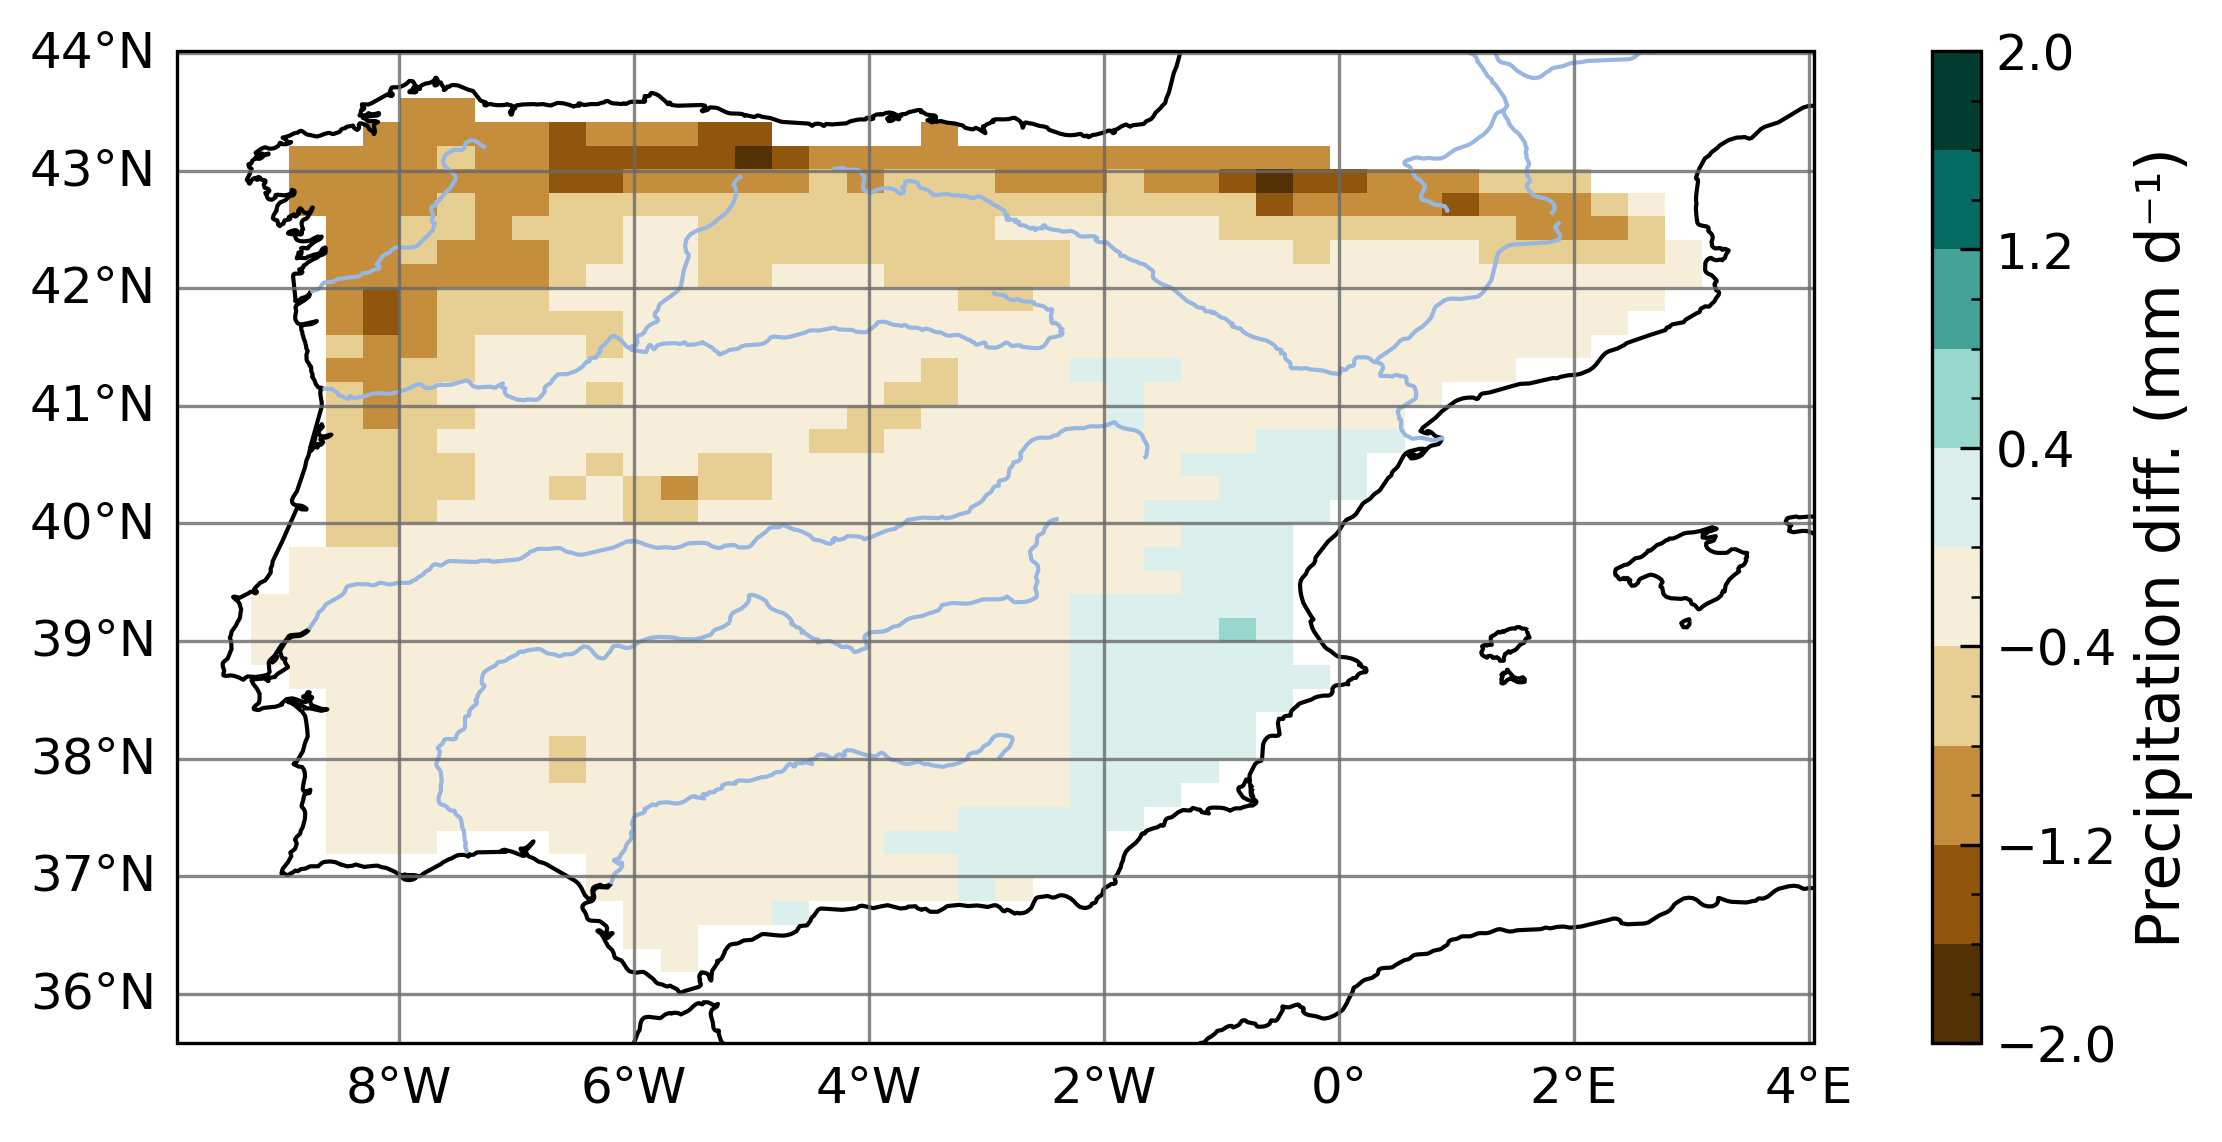
\includegraphics[width=\textwidth]{images/chap4/future/diffmap_precip_presfut.png}
        \end{subfigure} &
        %evap
        \begin{subfigure}[b]{0.5\textwidth}
            \caption{ET difference}
            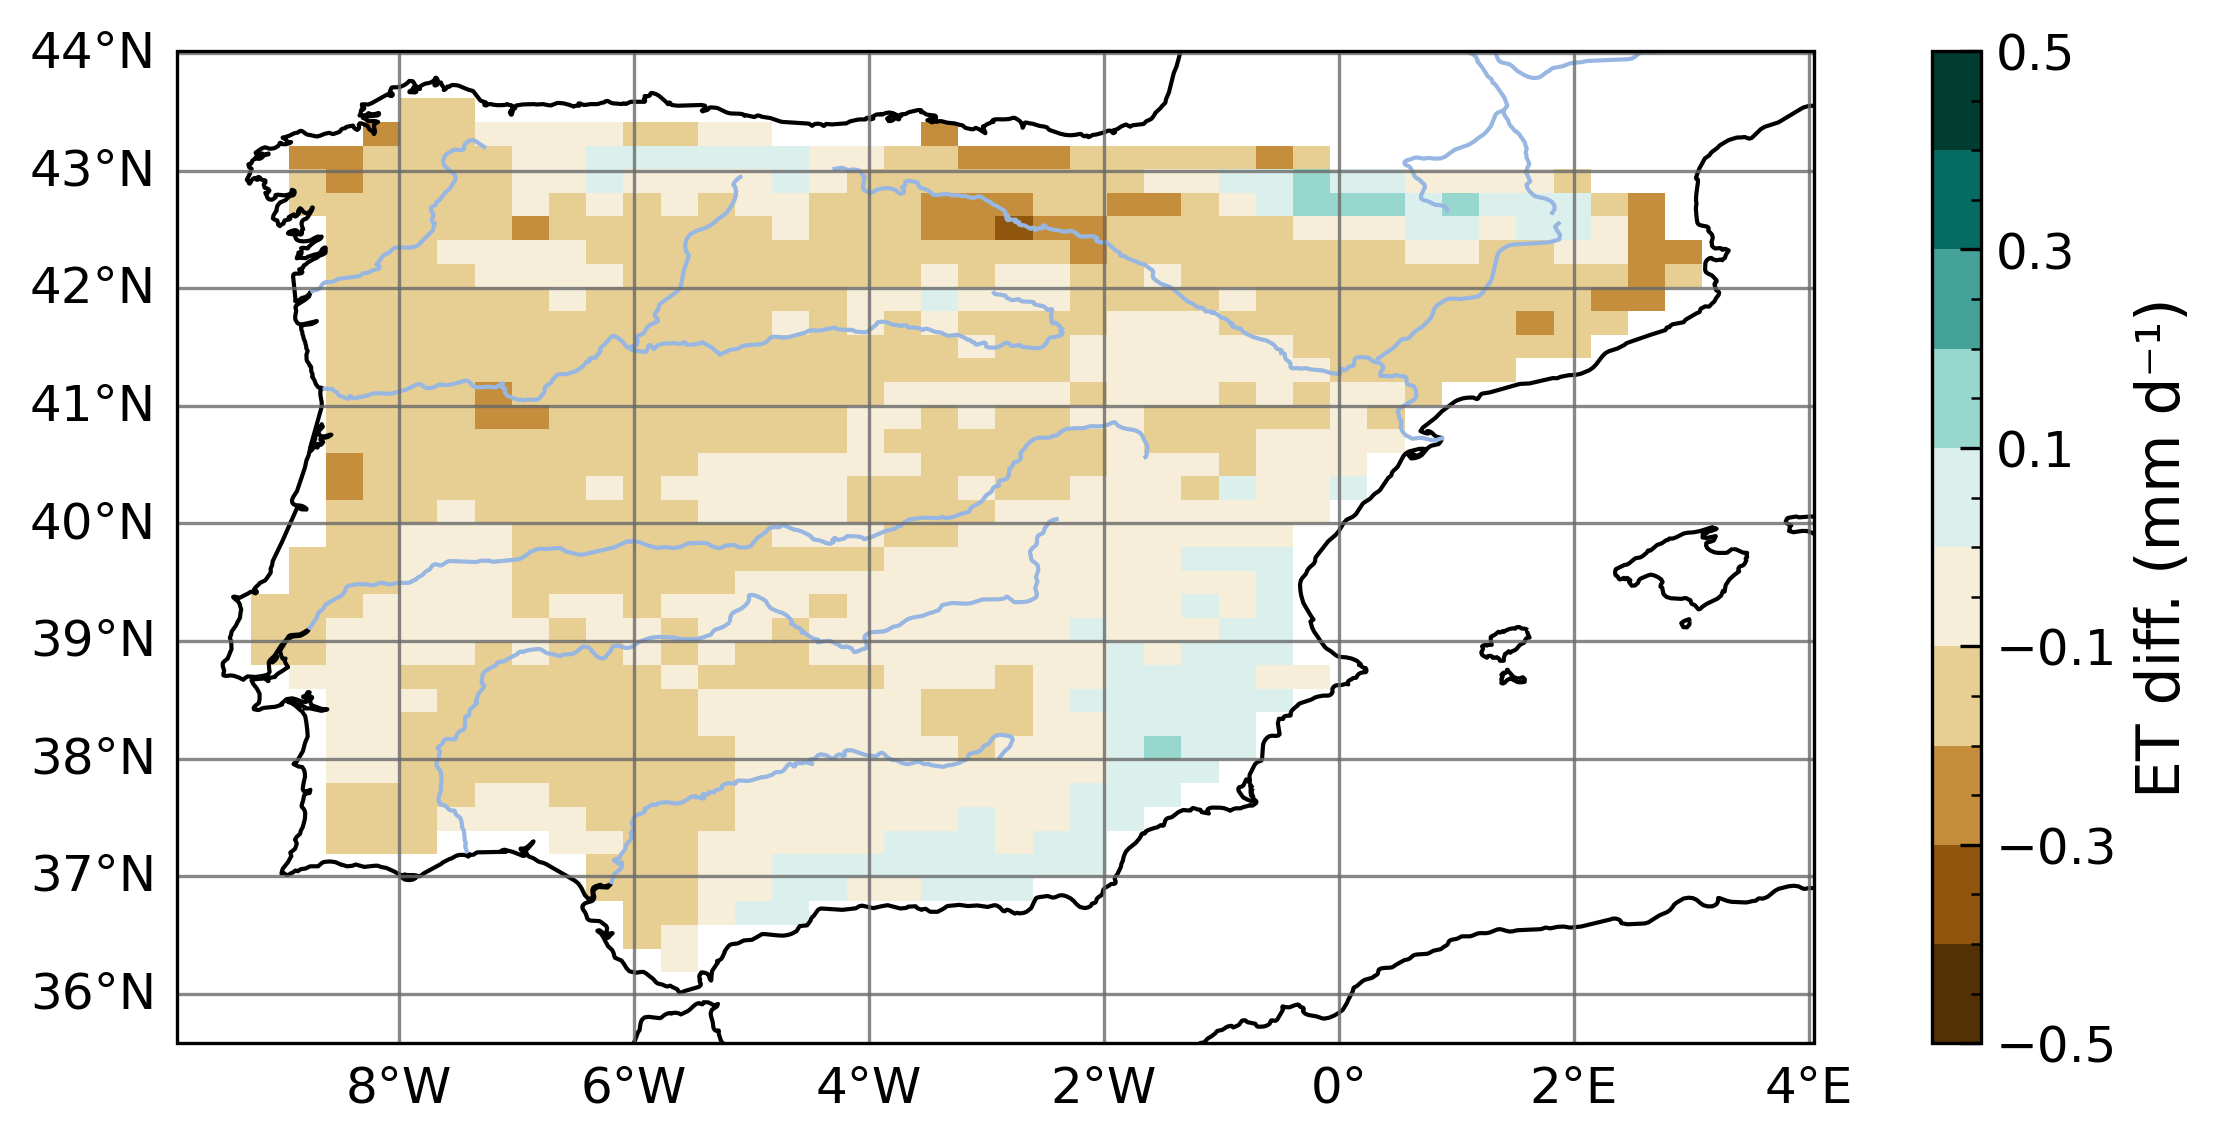
\includegraphics[width=\textwidth]{images/chap4/future/diffmap_evap_presfut.png}
        \end{subfigure} \\


        %q2m
        \begin{subfigure}[b]{0.5\textwidth}
            \caption{2-m specific humidity difference}
            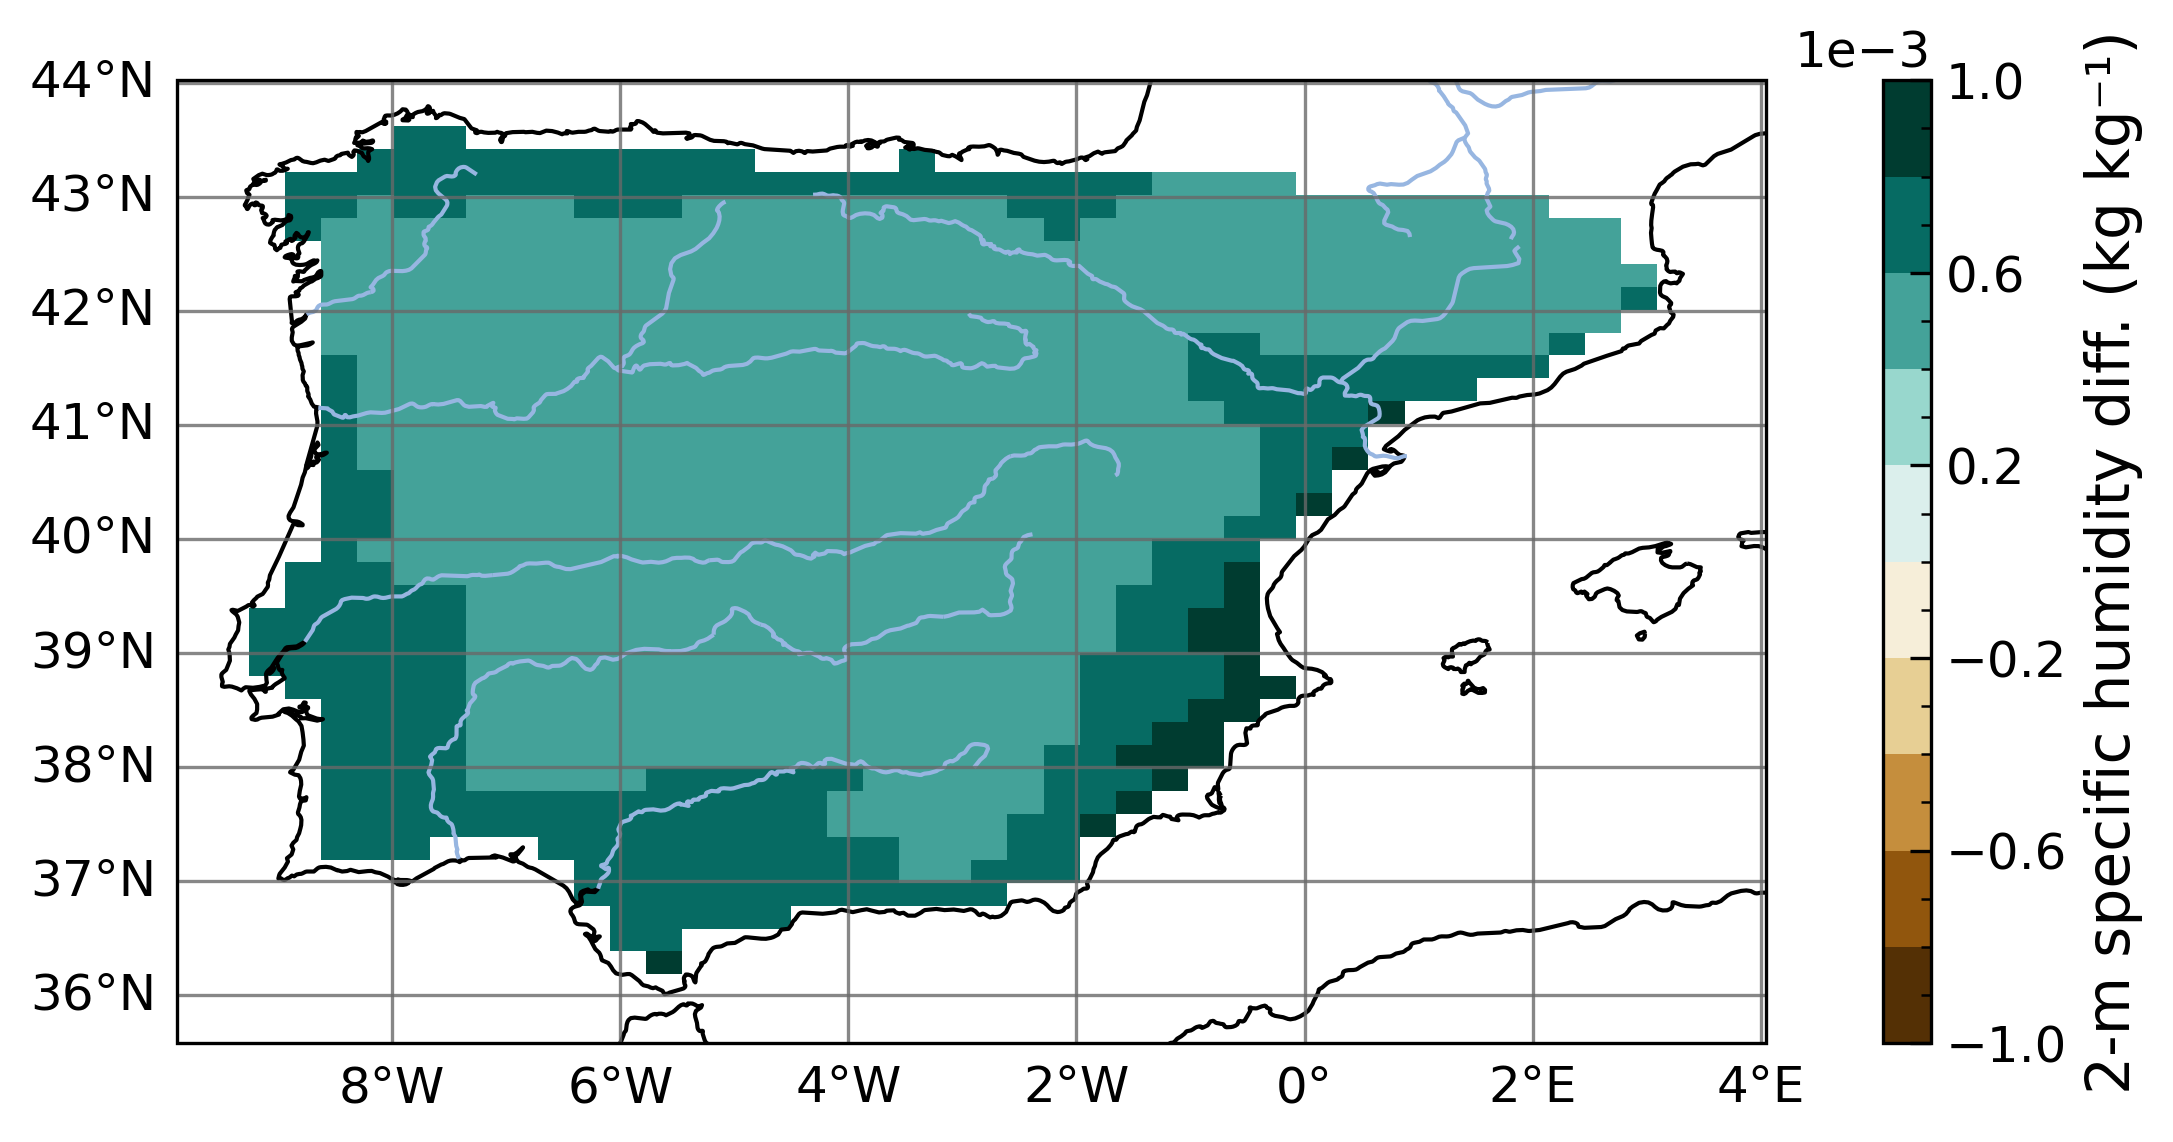
\includegraphics[width=\textwidth]{images/chap4/future/diffmap_q2m_presfut.png}
        \end{subfigure} &
        %rh2m
        \begin{subfigure}[b]{0.5\textwidth}
            \caption{2-m relative humidity difference}
            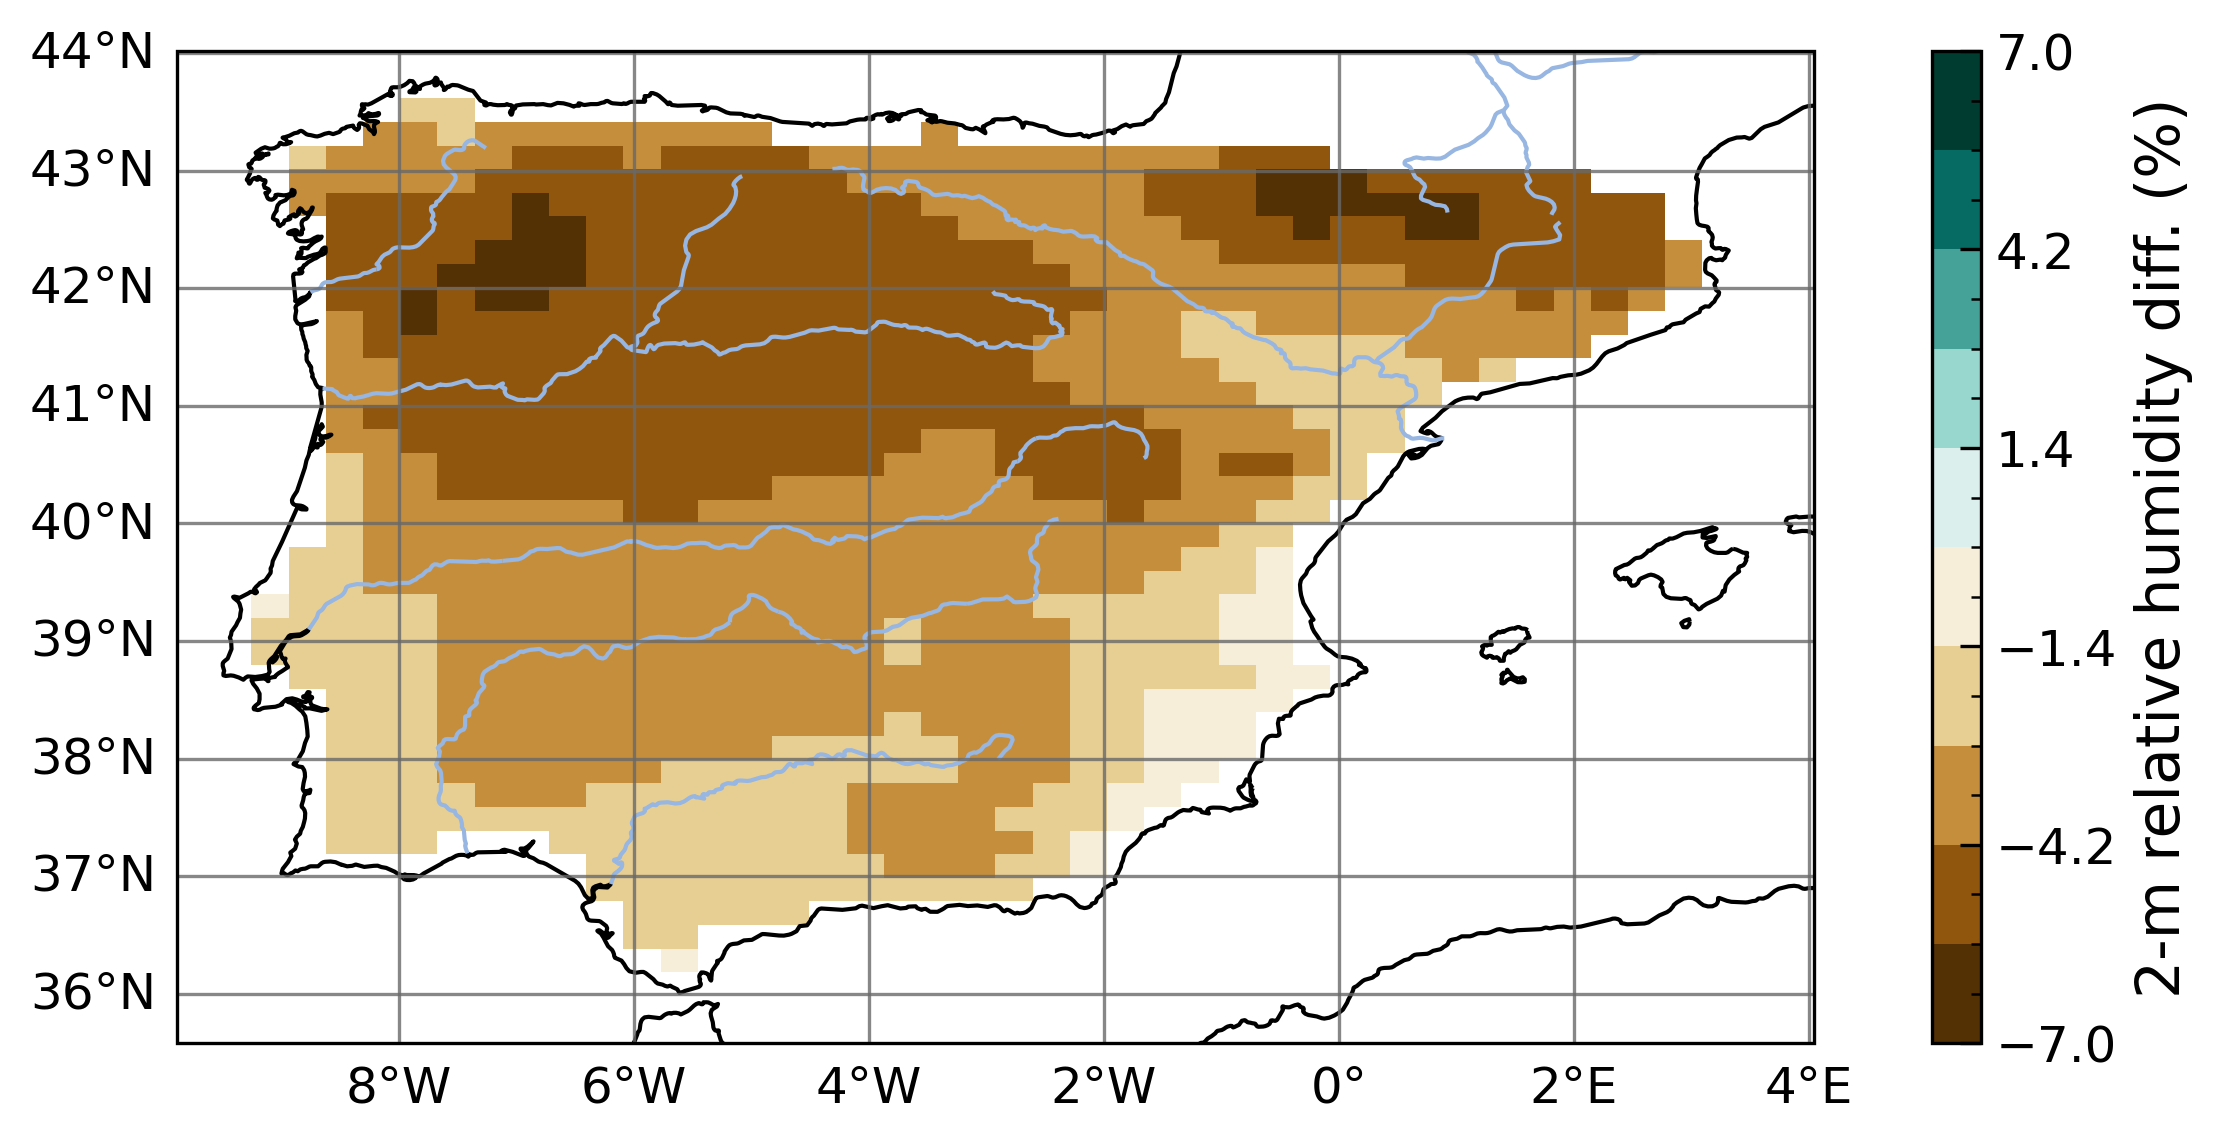
\includegraphics[width=\textwidth]{images/chap4/future/diffmap_rh2m_presfut.png}
        \end{subfigure} \\

        %SWdnSFC
        \begin{subfigure}[b]{0.5\textwidth}
            \caption{Downwelling shortwave radiation difference}
            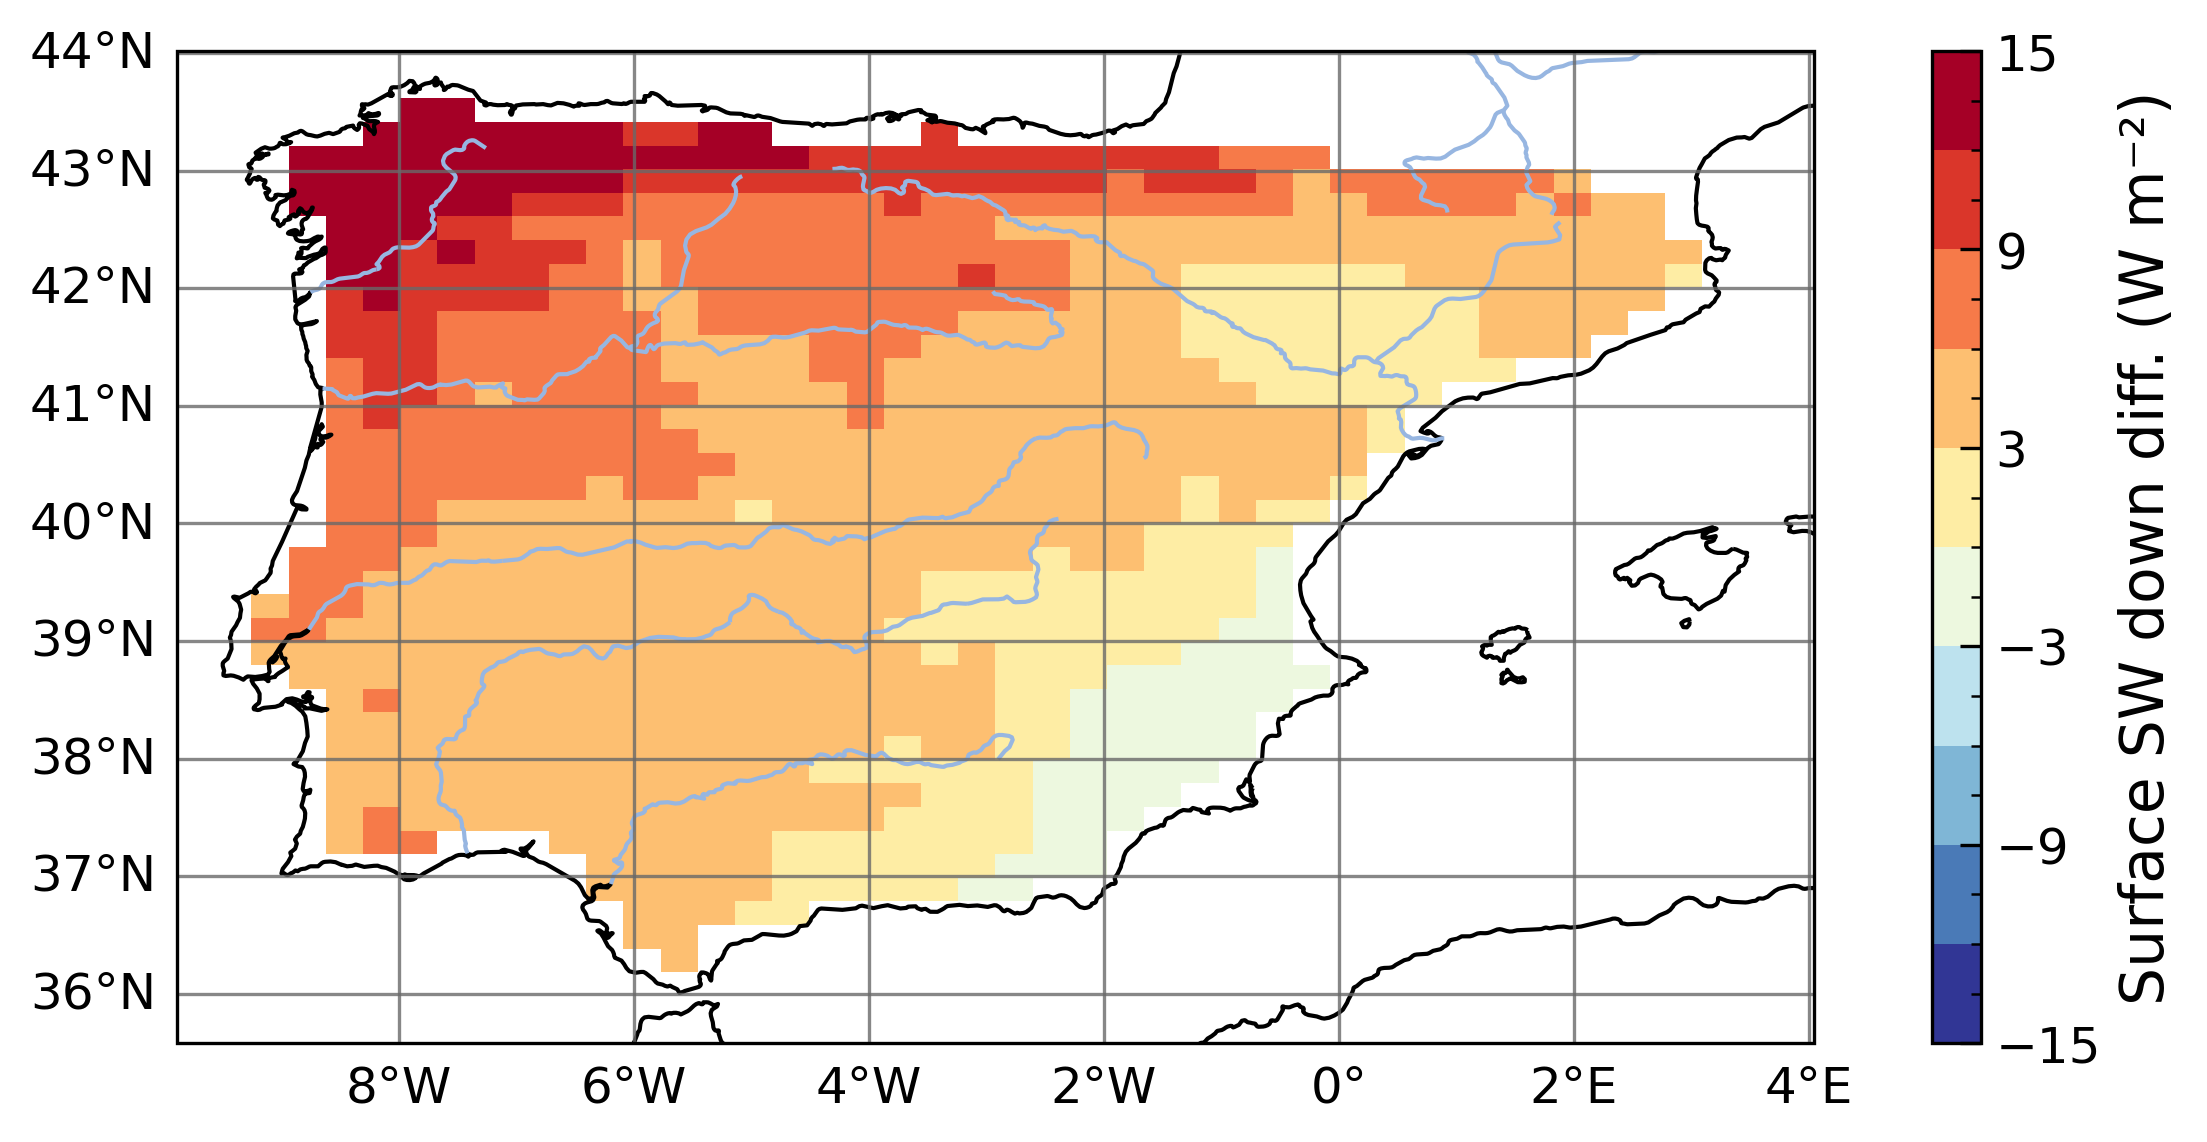
\includegraphics[width=\textwidth]{images/chap4/future/diffmap_SWdnSFC_presfut.png}
        \end{subfigure} &
        %LWdnSFC
        \begin{subfigure}[b]{0.5\textwidth}
            \caption{Downwelling longwave radiation difference}
            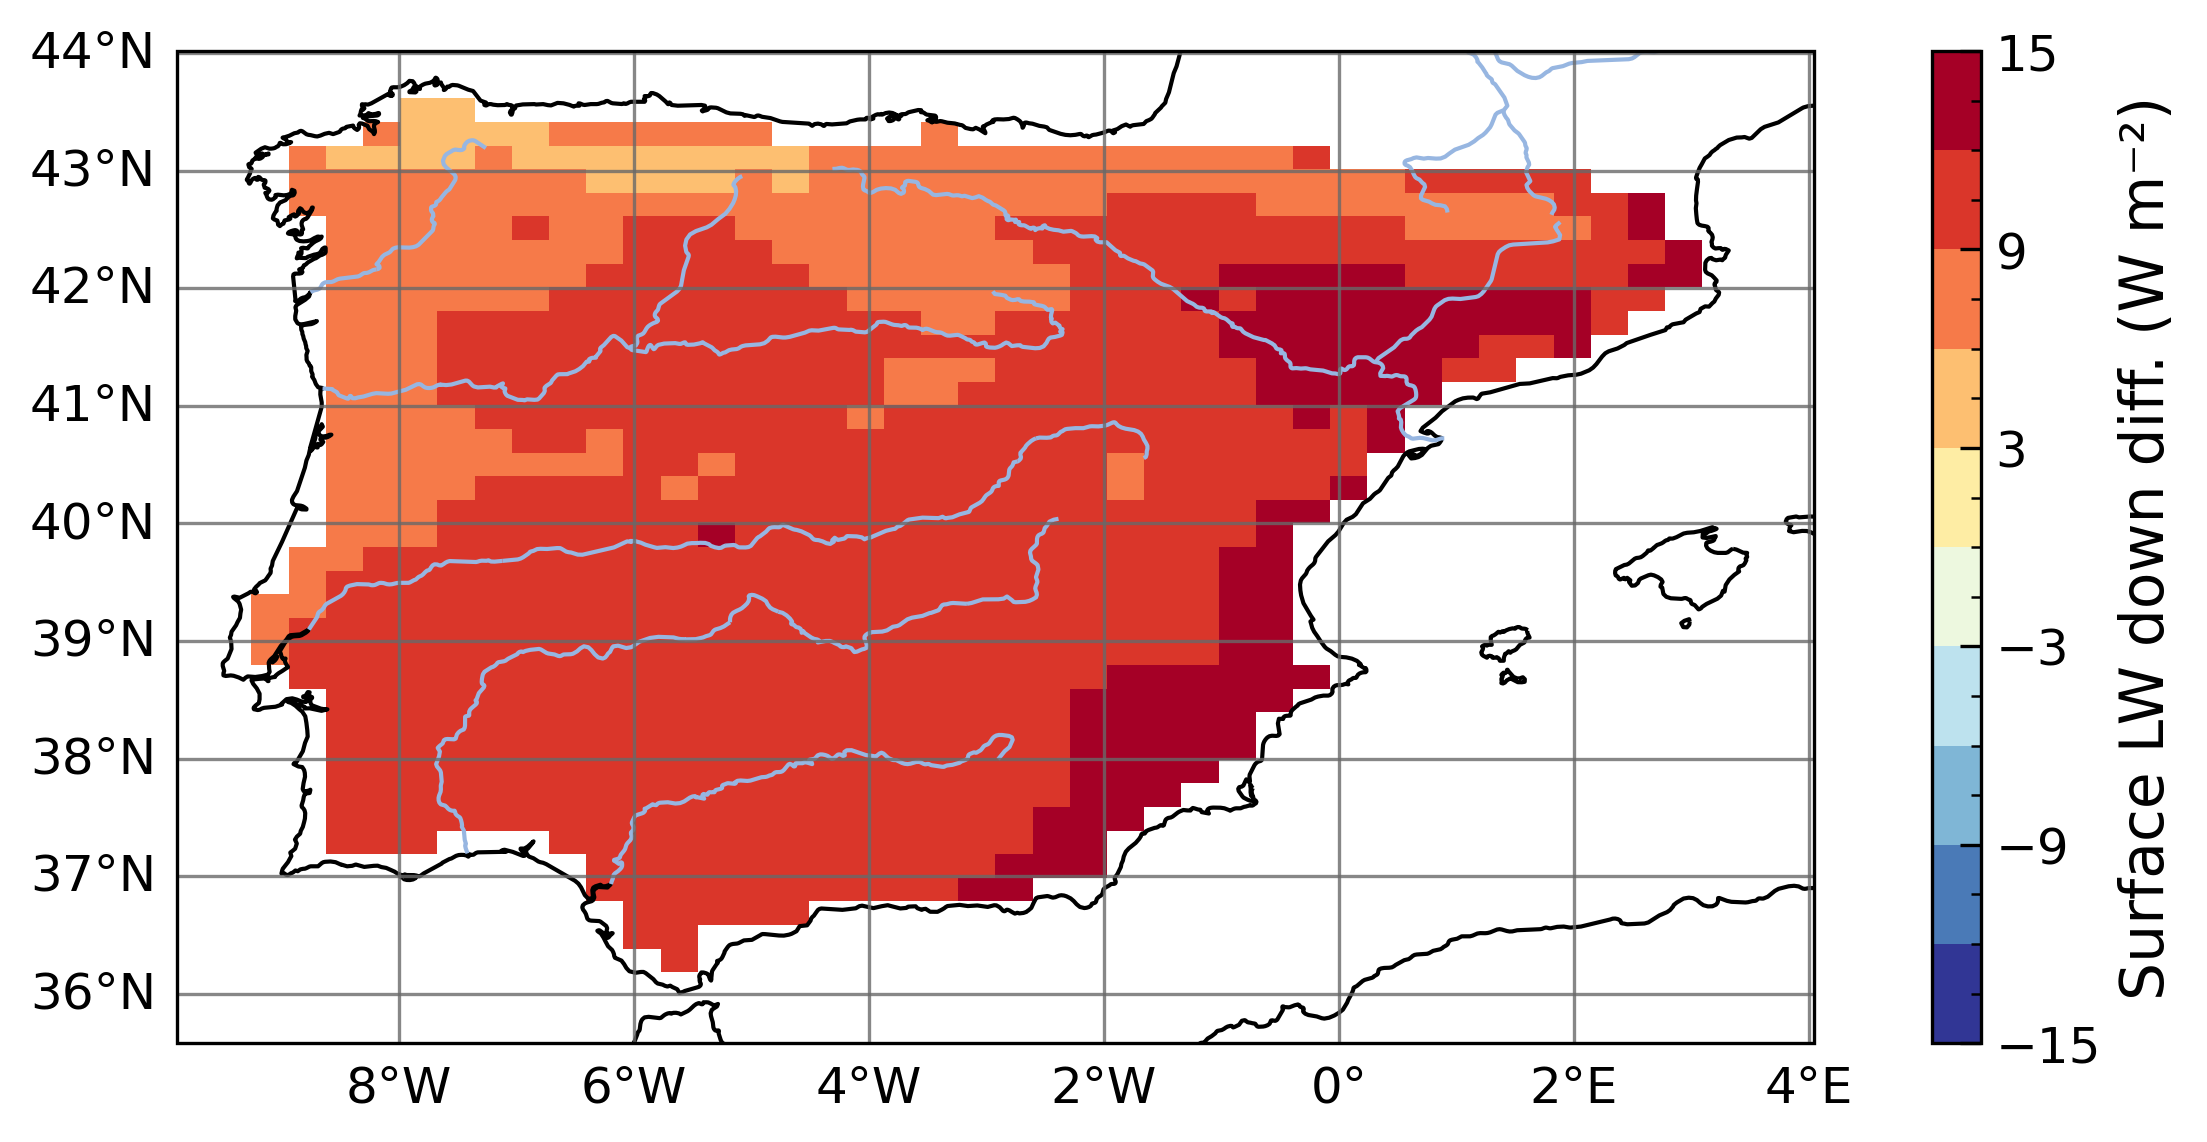
\includegraphics[width=\textwidth]{images/chap4/future/diffmap_LWdnSFC_presfut.png}
        \end{subfigure} \\

        % %pblh
        % \begin{subfigure}[b]{0.5\textwidth}
        %     \caption{}
        %     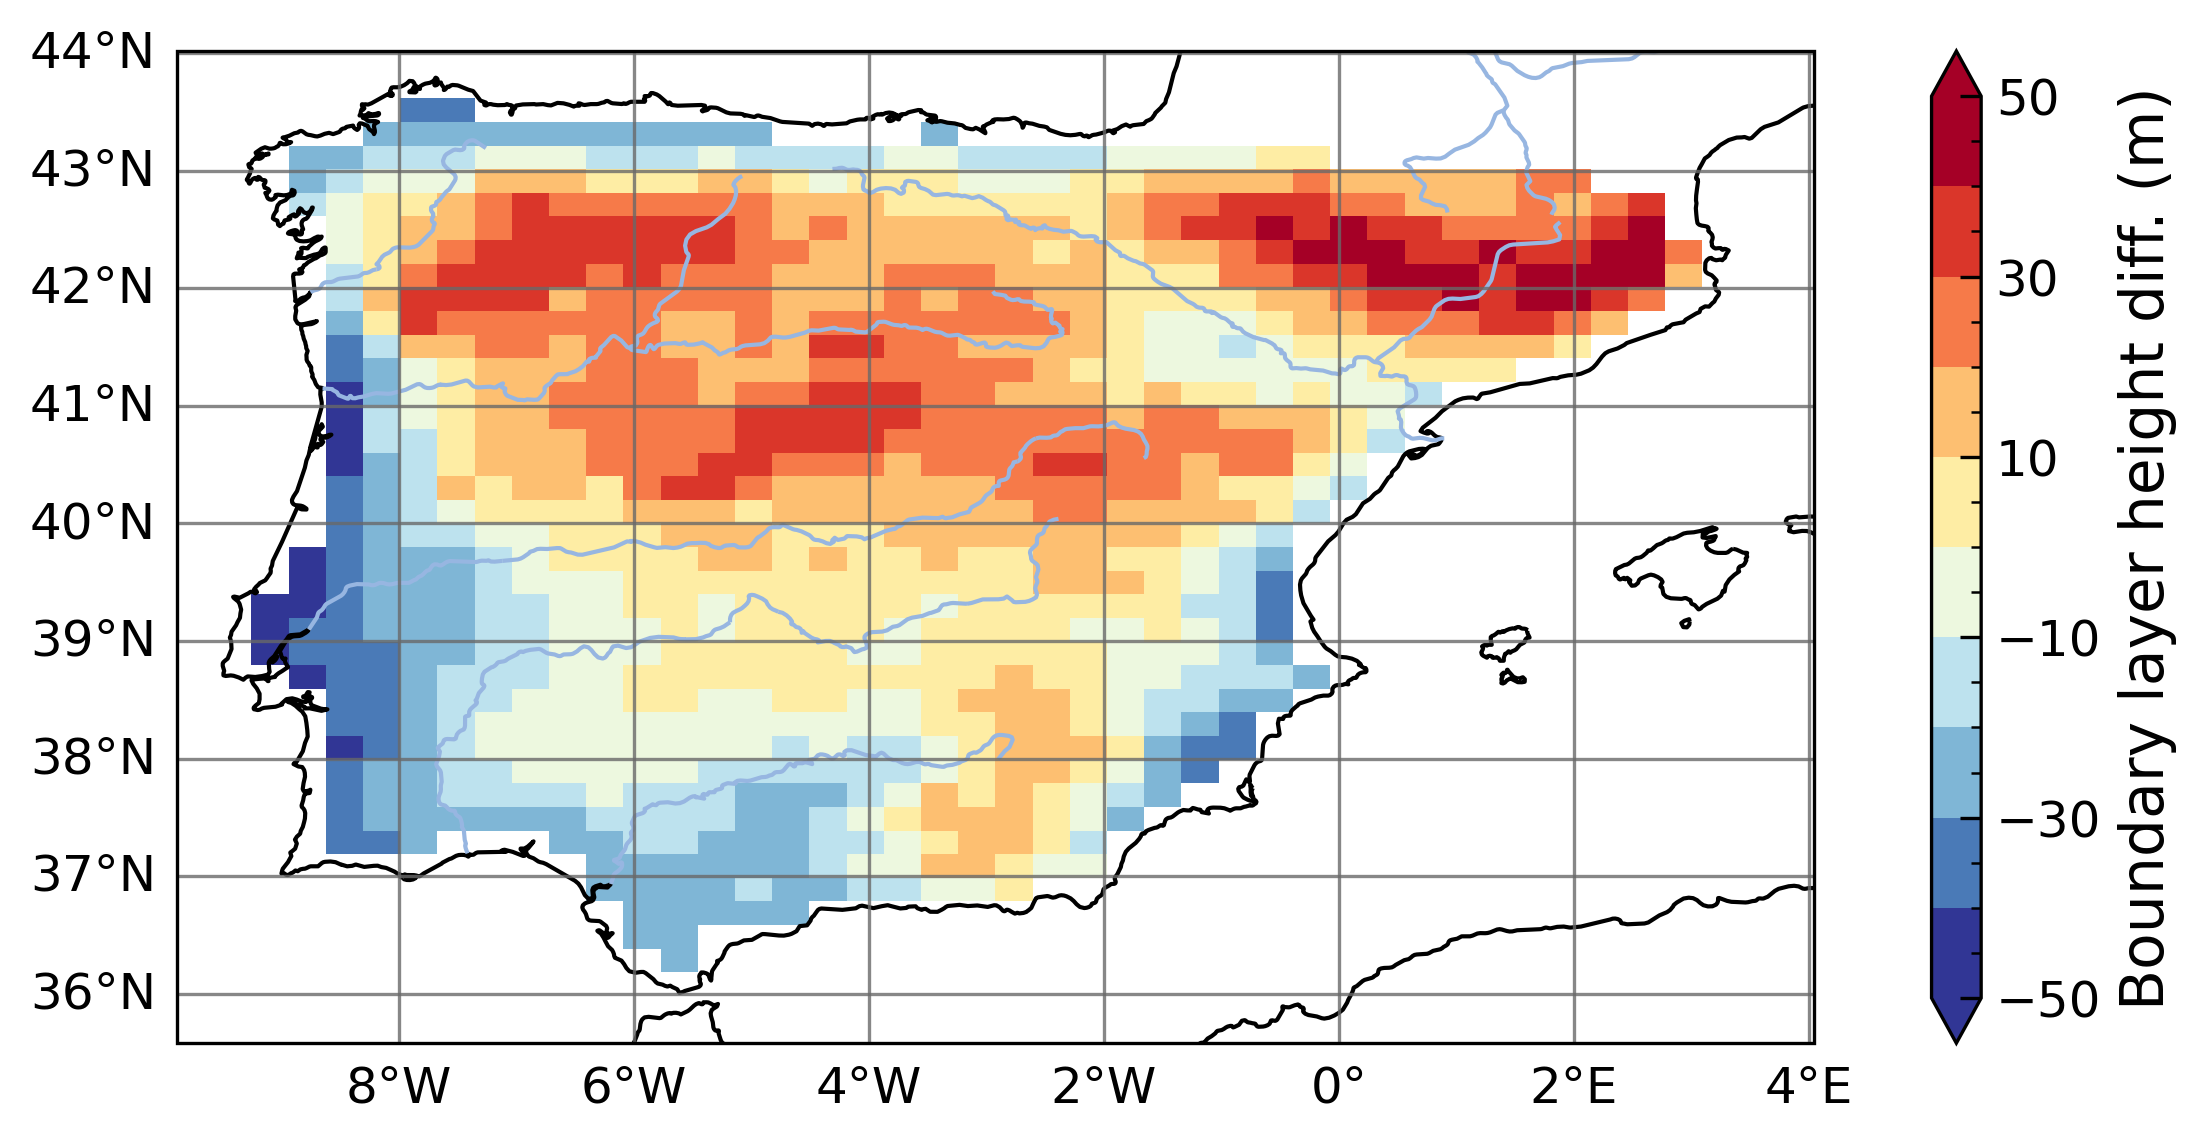
\includegraphics[width=\textwidth]{images/chap4/future/diffmap_s_pblh_presfut.png}
        % \end{subfigure} &
        % %lcl
        % \begin{subfigure}[b]{0.5\textwidth}
        %     \caption{}
        %     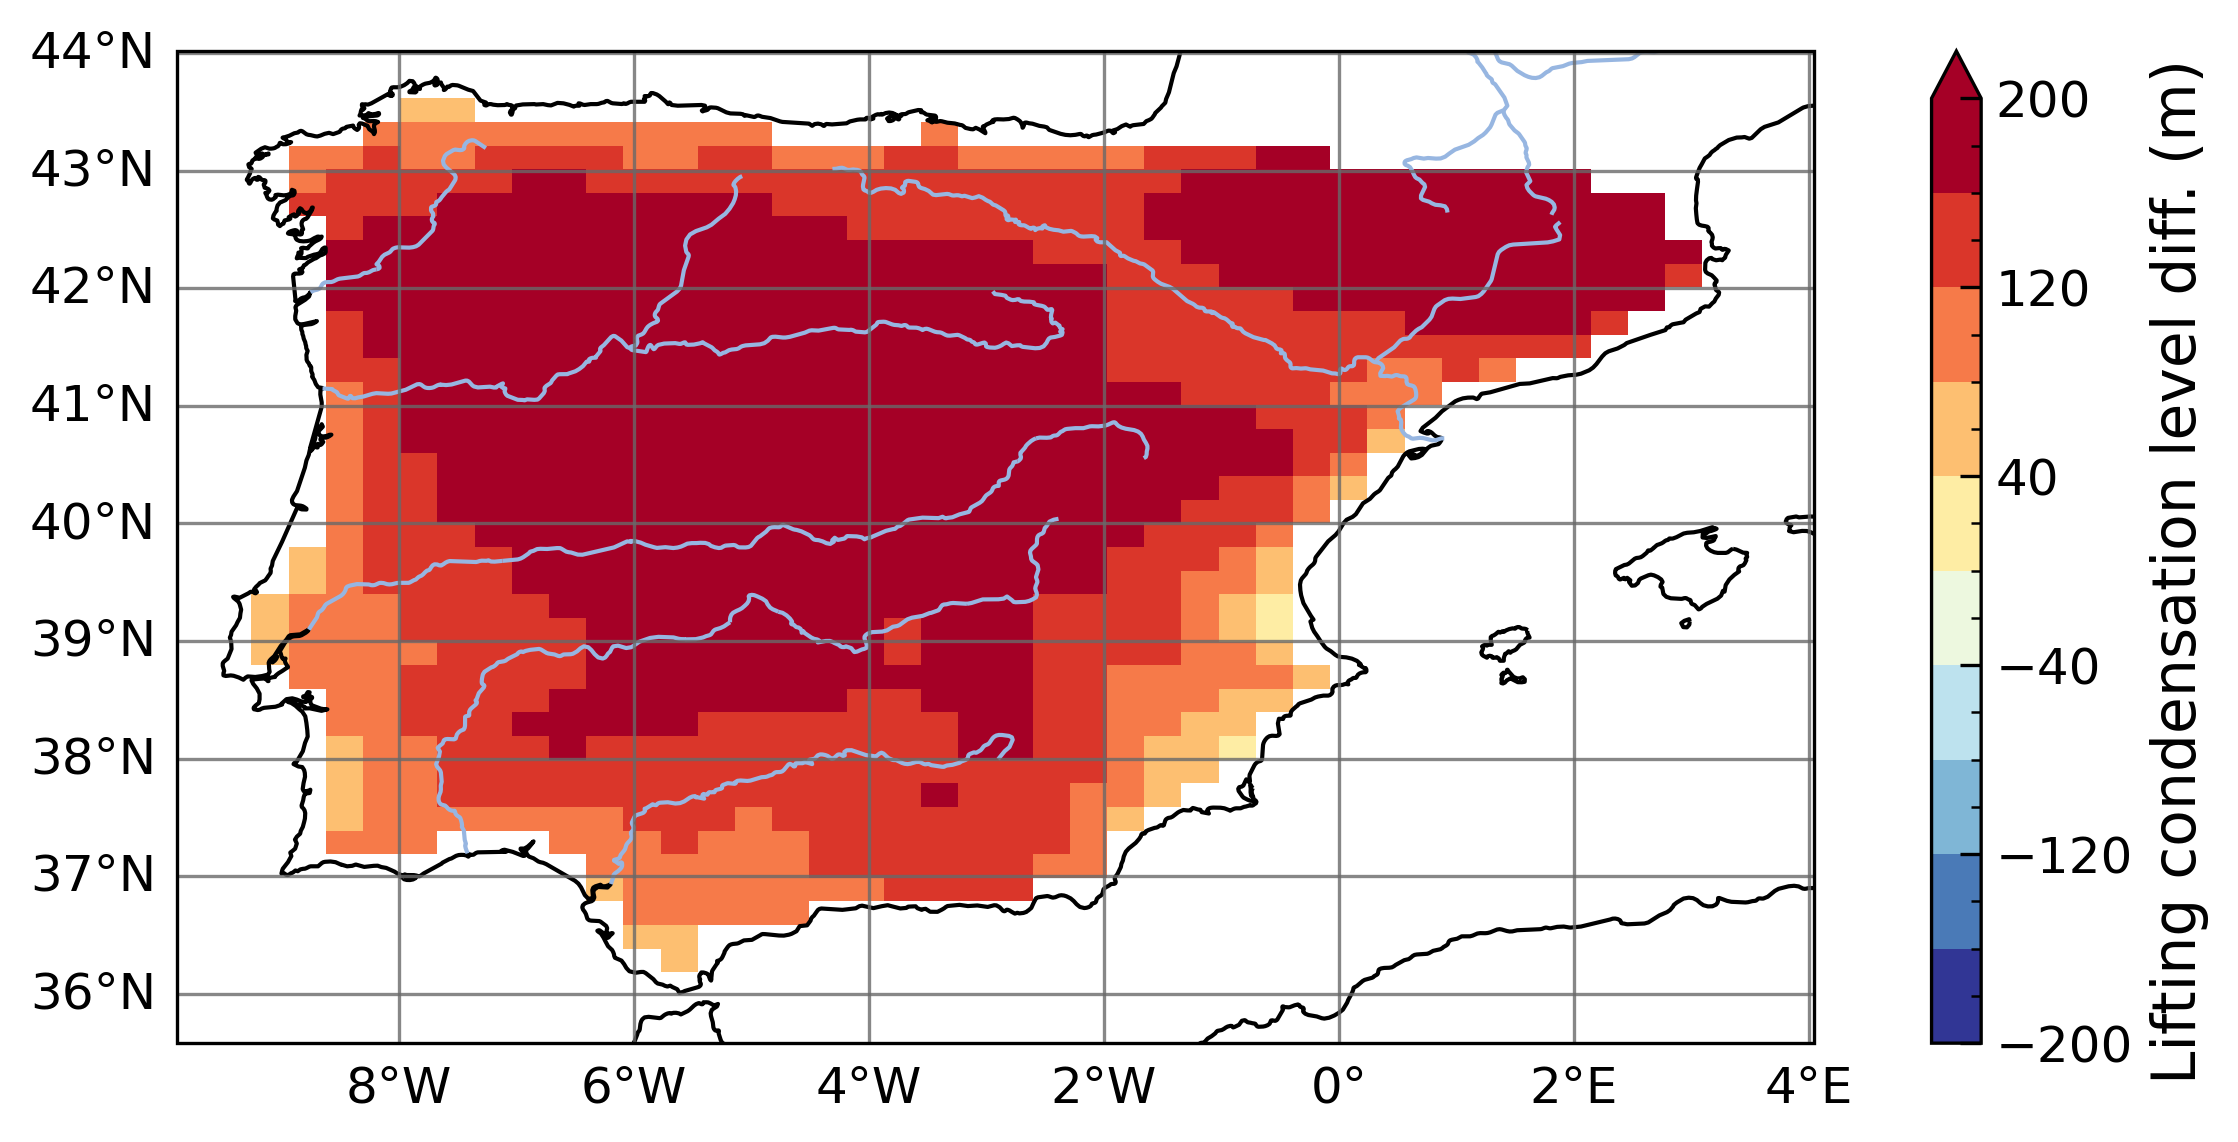
\includegraphics[width=\textwidth]{images/chap4/future/diffmap_s_lcl_presfut.png}
        % \end{subfigure} \\
    \end{tabular}
    \caption{Impacts of climate change over the Iberian Peninsula. Annual mean difference between \futnoirr (2050-2062) and  \presnoirr (2010-2022).}
    \label{fig:diffmaps_present_future}
\end{figure}

\clearpage

\subsection{Impacts of irrigation under climate change}

%figure : map and SC of irrigation in the future
\begin{figure}[htbp]
    \centering
    \begin{tabular}{cc}
        %precip
        \begin{subfigure}[b]{0.48\textwidth}
            \caption{Irrigation annual mean}
            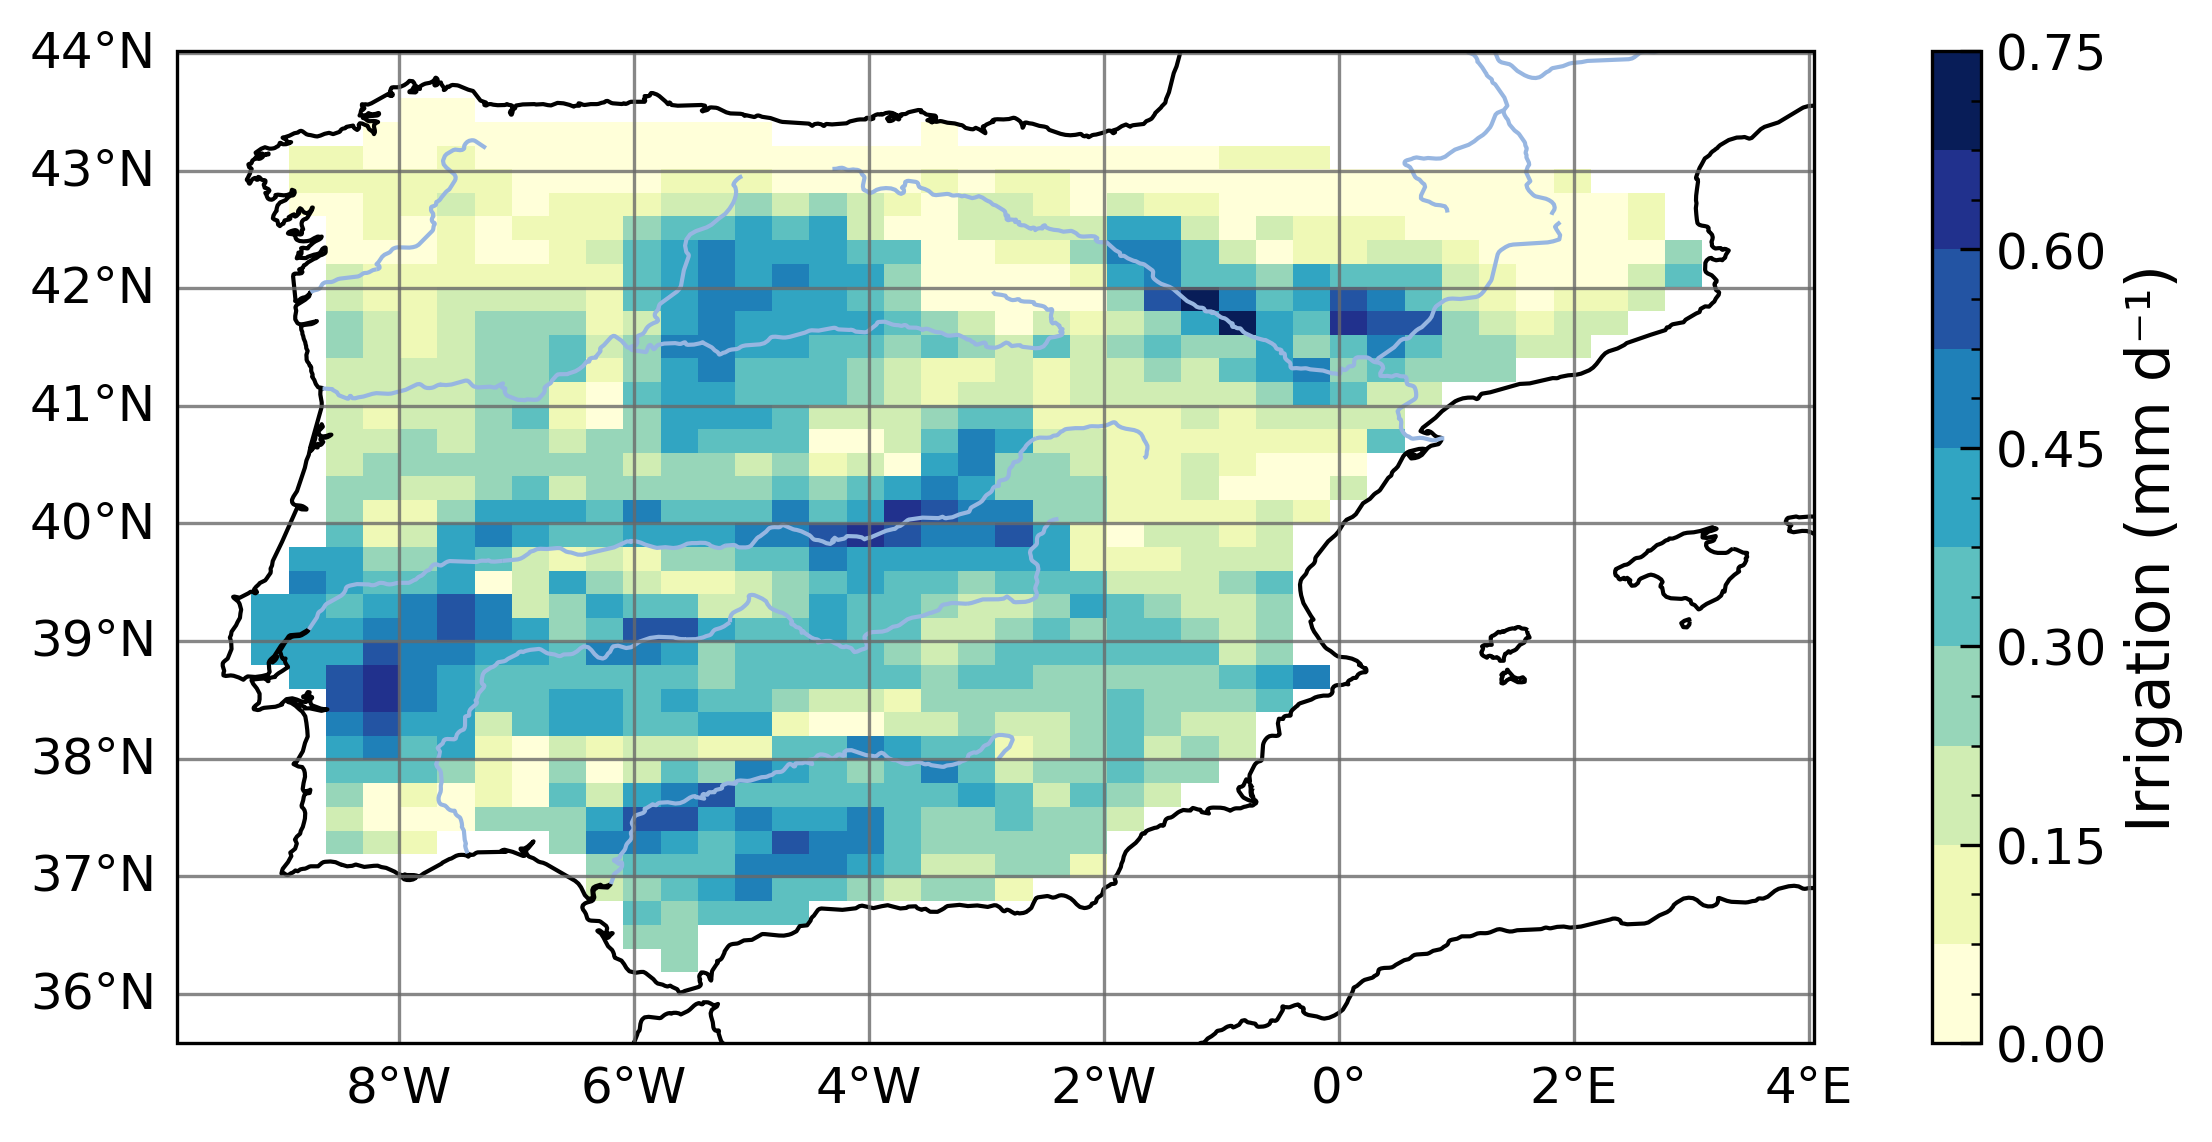
\includegraphics[width=\textwidth]{images/chap4/future/map_irrigation_fut.png}
        \end{subfigure} &
        \begin{subfigure}[b]{0.46\textwidth}
            \caption{Irrigation mean seasonal cycle}
            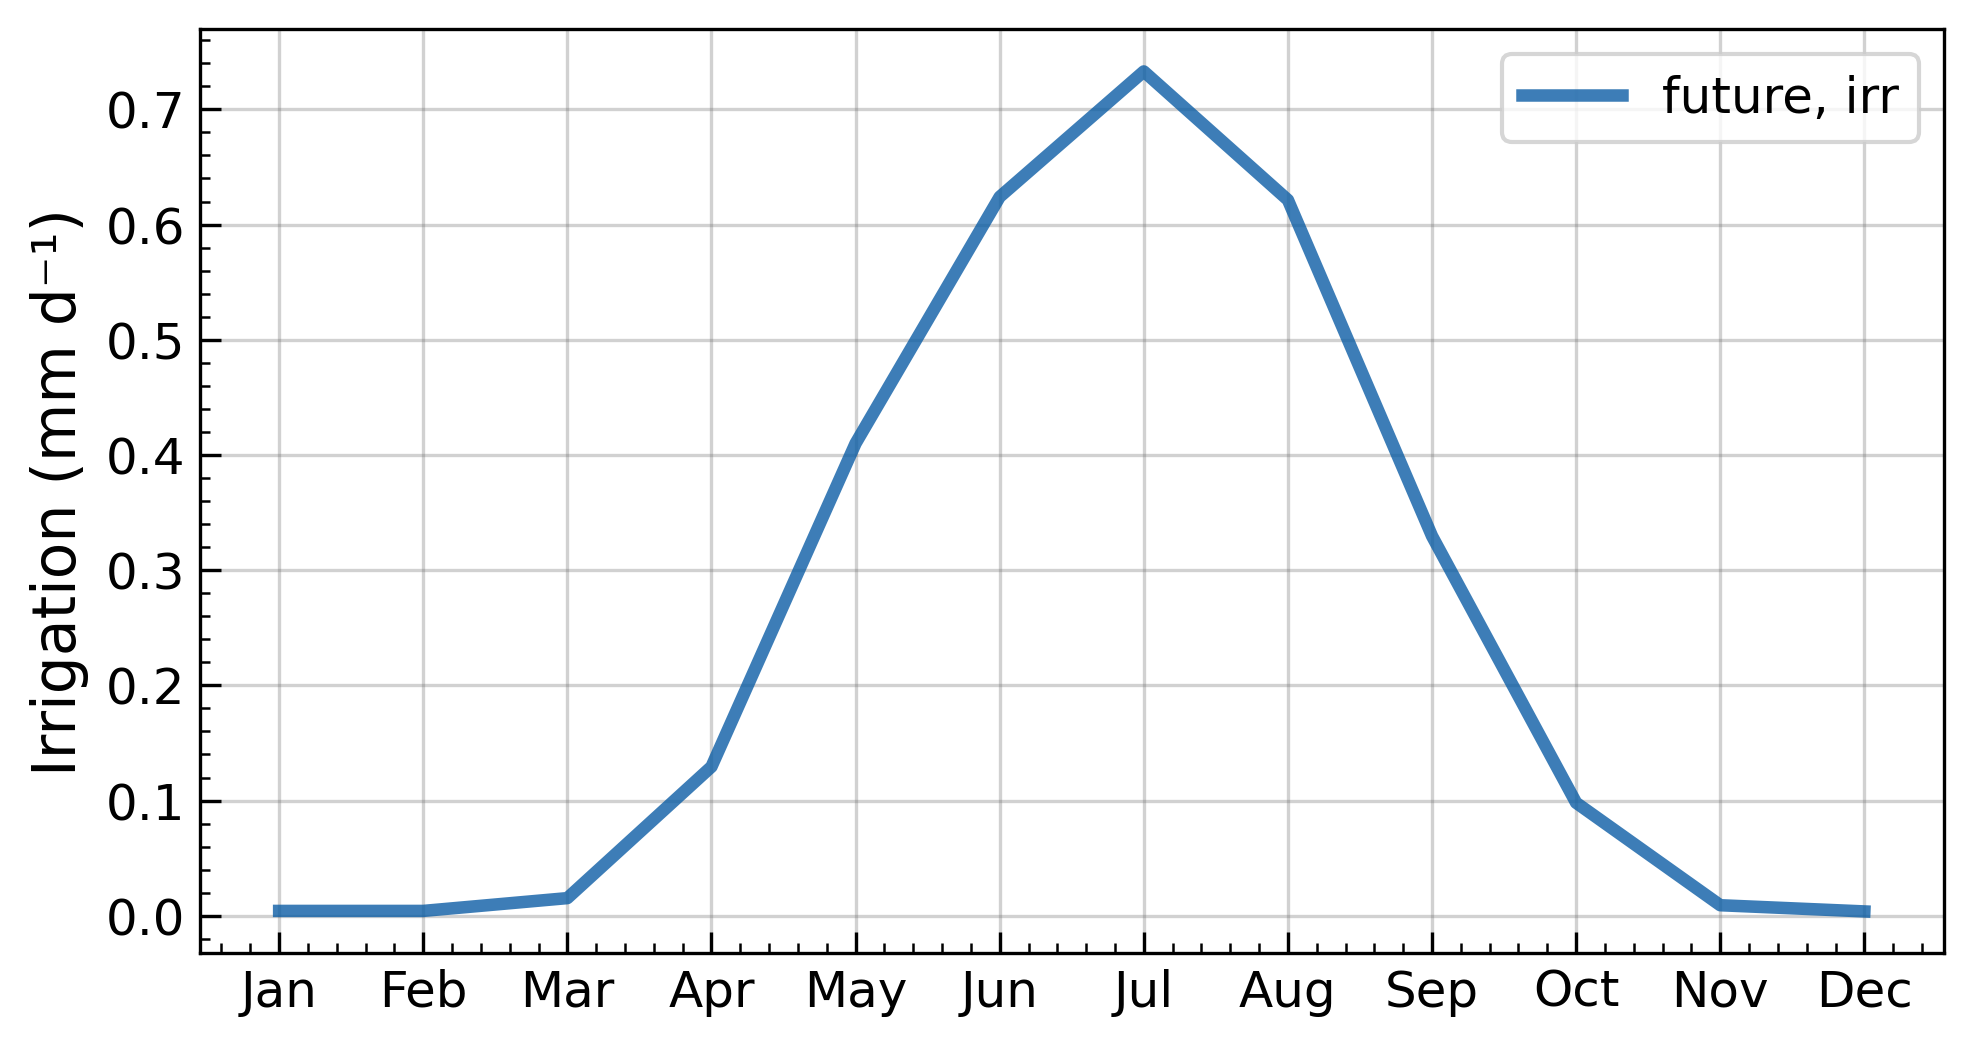
\includegraphics[width=\textwidth]{images/chap4/future/SC_irrigation_fut.png}
        \end{subfigure}
    \end{tabular}
    \caption{Annual mean and seasonal cycle of irrigation over the Iberian Peninsula in the \futirr simulation (2050-2062).}
    \label{fig:future_irrig}
\end{figure}

Irrigation in the \futirr simulation is largest in the valleys of the Ebro, Douro, Tagus, Guadiana and Guadalquivir rivers (Fig. \ref{fig:future_irrig}a). Due to modelling choices, it is near-zero in winter, and follows a rather symmetrical seasonal cycle from spring to autumn, with a peak in July (Fig. \ref{fig:future_irrig}b).
%option: direct comparison with simulated irrigation in present ? Tricky : one big difference is the forcing used (ERA5 vs ICOLMDZOR) ; another is the fact that for this simulation, routing was inappropriately paramterized, leading to huge volumes in reservoirs... (new simulation with same parameters ongoing...)

%turbulent fluxes
Its most direct atmospheric impact is an increase in ET of similar amplitude to the irrigation amounts (Fig. \ref{fig:diffmaps_future_irr}d), which largely compensates for the decrease in ET induced by climate change. This increase of the latent heat flux is directly linked to a decrease of the sensible heat flux (Fig. \ref{fig:diffmaps_future_irr}b) reaching -15 W \persqm in the most irrigated valleys. 
%t2m
This new partitionning of surface energy leads to a cooler air over most of the domain (Fig. \ref{fig:diffmaps_future_irr}a). The largest decreases occur  over the intensely irrigated areas where 2-m temperature is lowered by 0.5°C on annual average and 1°C in summer. %todo:appendix figure or remove ?
Contrary to ET, this consequence of irrigation is insufficient to compensate the impact of climate change, which induces 2-m temperature increases of 2°C annually and larger than 3°C in summer. %todo:appendix figure or remove ?
%q2m RH2m
Regarding humidity, \futirr is moister than \futnoirr (Fig. \ref{fig:diffmaps_future_irr}e) but some intensely irrigated areas such as the Ebro valley show smaller increases in specific humidity than others, suggesting a stronger mixing of the lower atmosphere in these regions. Combined with the changes in temperature, the increase of specific humidity also leads to an increase in relative humidity  (Fig. \ref{fig:diffmaps_future_irr}f), wich opposes the impact of climate change.
%ABL
The structure of the boundary layer is also affected by irrigation. Stabilization dominates and follows the same pattern as irrigation, as a consequence of cooling and of the reduced sensible heat flux. The ABL height is lowered by more than a 100m in the most intensely irrigated grid areas. 
Due to the moistening and cooling of the atmosphere, the lifting condensation level is also lowered. Similarly to the changes in 2-m humidity, LCL is more affected in the Tagus, Guadiana and Guadalquivir basins than in the Ebro and Douro basins.
As explained in Section \ref{sec:article1}, the lowering of both the ABL height and LCL point to to opposite effects on cloud formation and precipitation, since one reflects a more stable atmosphere less likely to form clouds through convection, while the other is associated with a moister and cooler atmosphere where condensation is more likely. As a consequence, the impact of irrigation on precipitation is rather limited and the only significant structures that emerge are precipitation increases in the highest moutain ranges, the Iberian System and the Pyrenees.

%figure : diff maps (future, irr - no_irr)
\begin{figure}[htbp]
    \centering
    \begin{tabular}{cc}
        %t2m
        \begin{subfigure}[b]{0.5\textwidth}
            \caption{2-m temperature difference}
            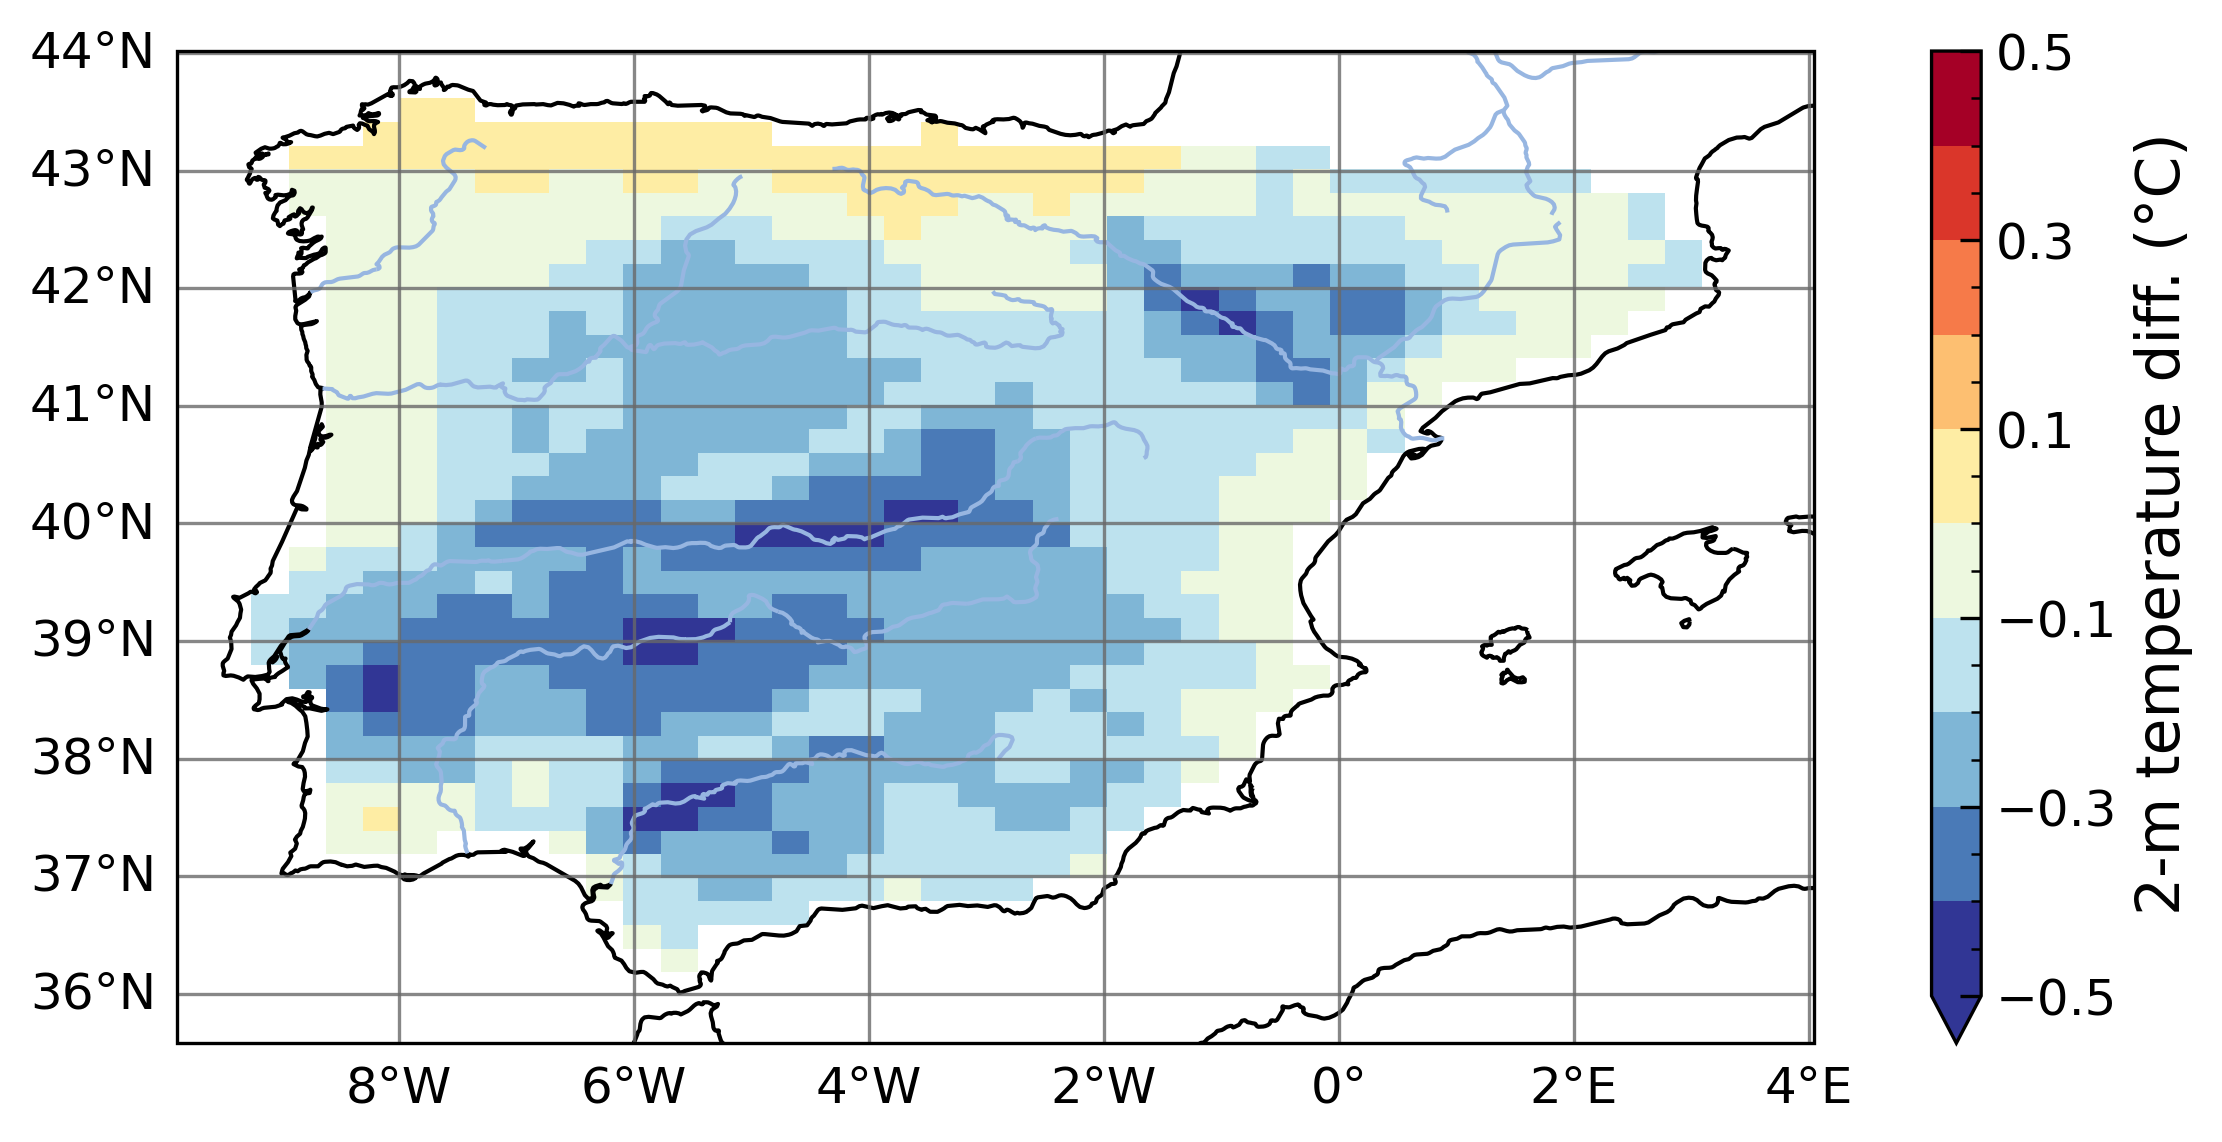
\includegraphics[width=\textwidth]{images/chap4/future/diffmap_t2m_futirr.png}
        \end{subfigure} &
        %fluxsens
        \begin{subfigure}[b]{0.5\textwidth}
            \caption{Sensible heat flux difference}
            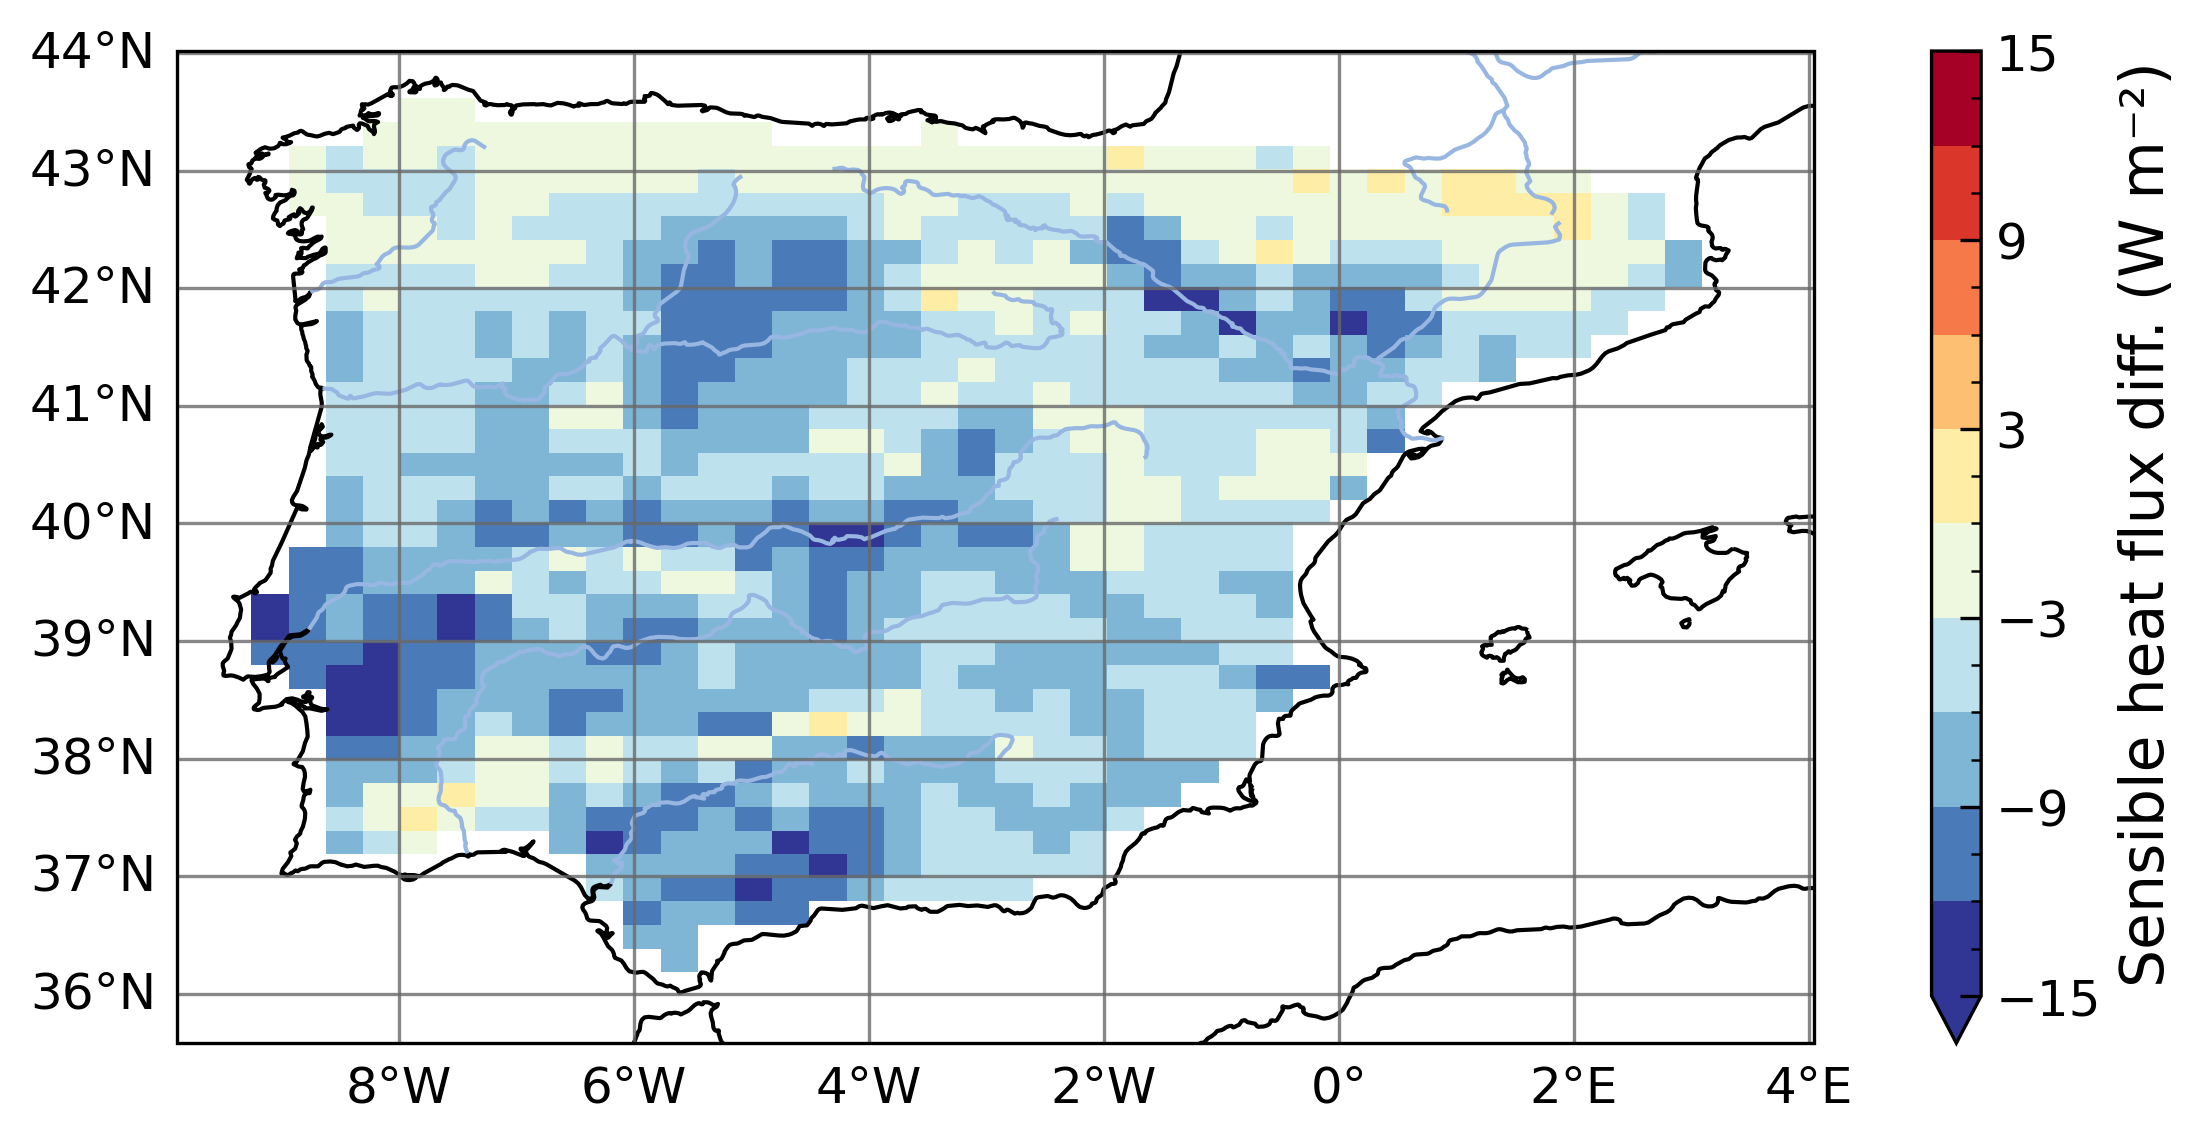
\includegraphics[width=\textwidth]{images/chap4/future/diffmap_fluxsens_futirr.png}
        \end{subfigure} \\

        %precip
        \begin{subfigure}[b]{0.5\textwidth}
            \caption{Precipitation difference}
            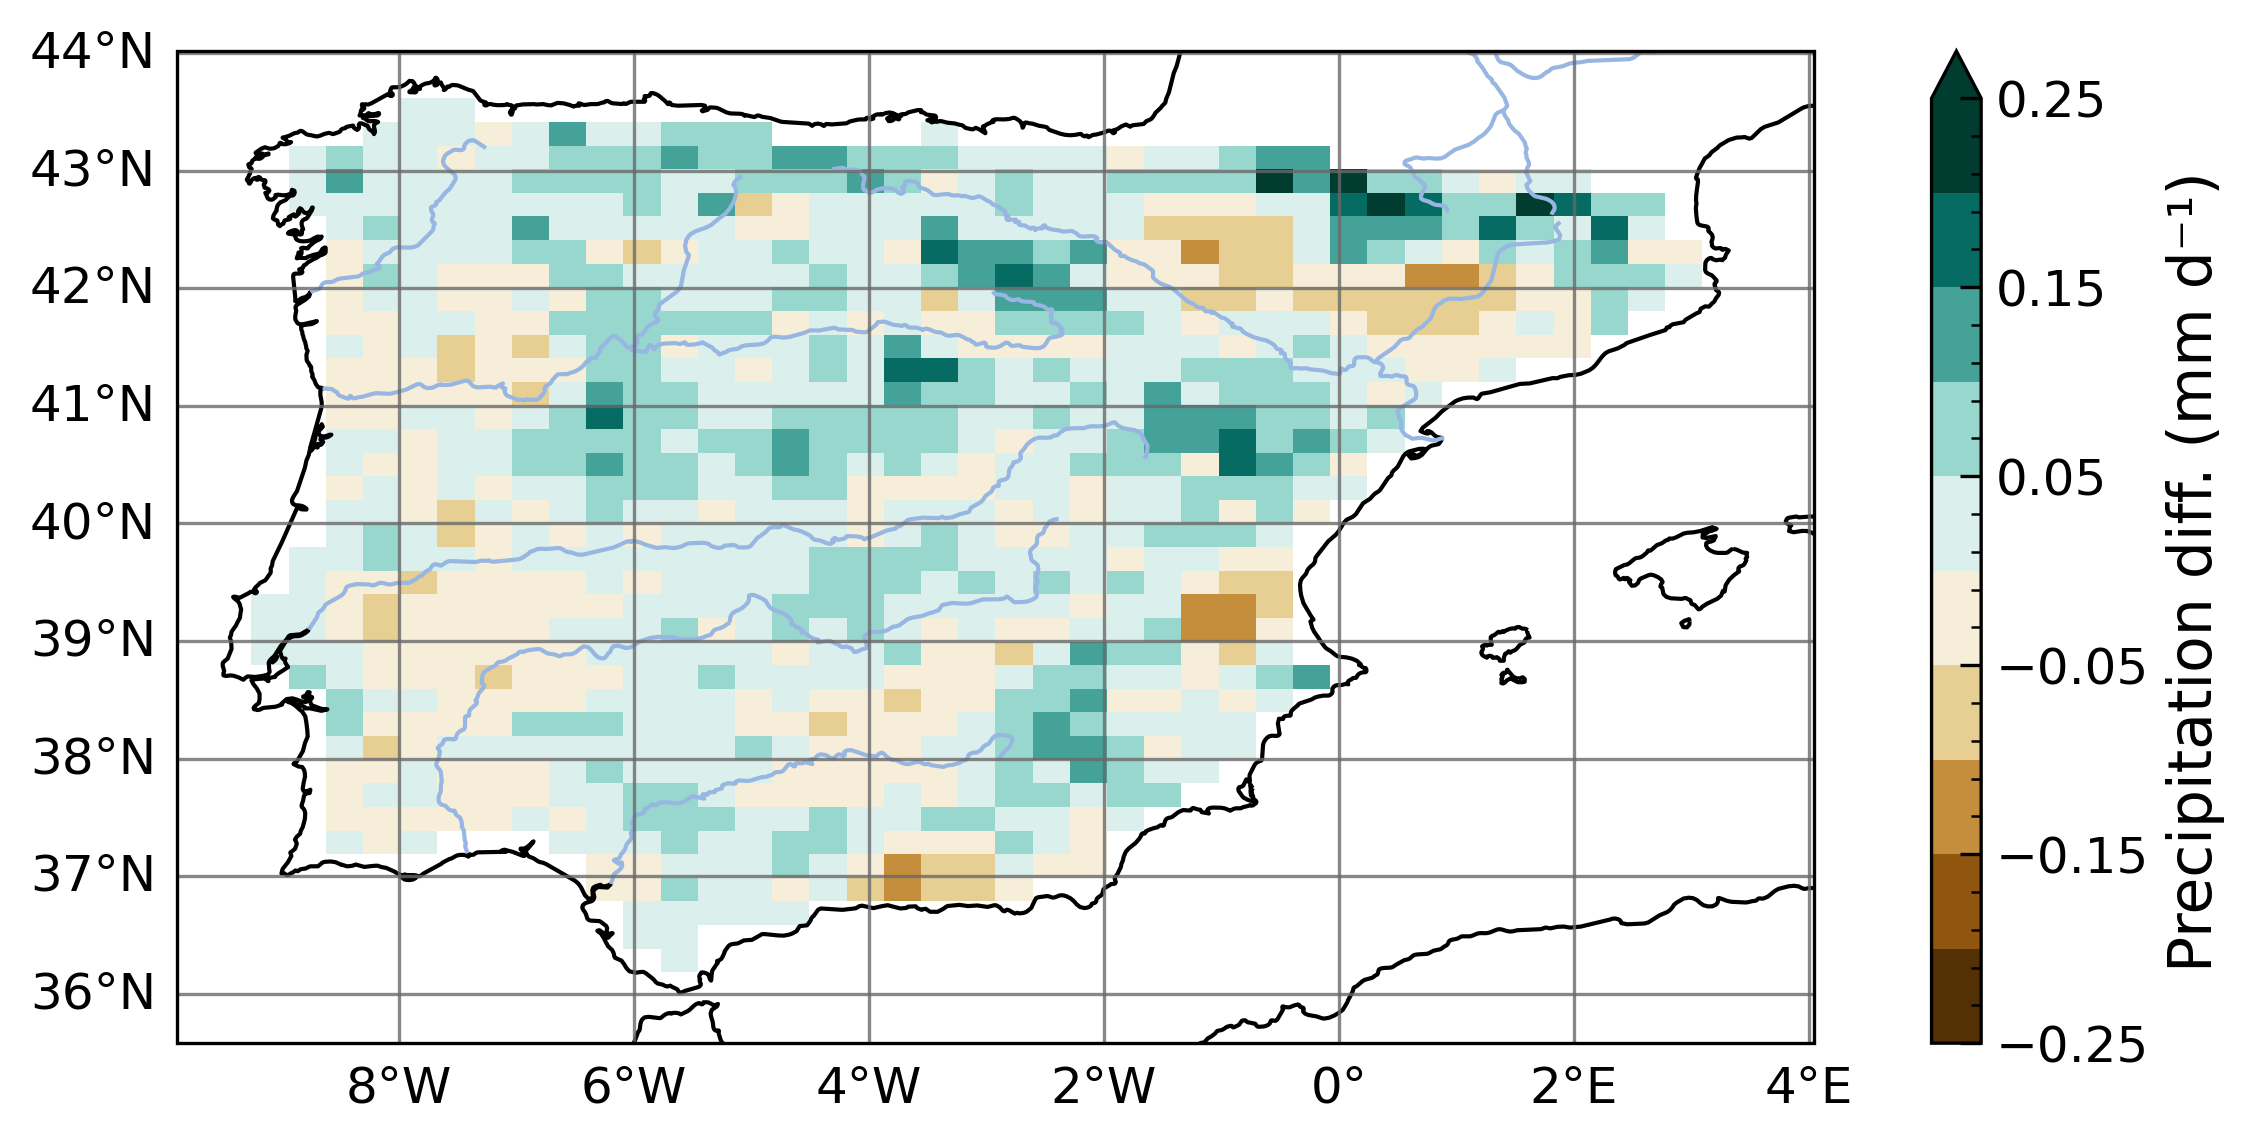
\includegraphics[width=\textwidth]{images/chap4/future/diffmap_precip_futirr.png}
        \end{subfigure} &
        %evap
        \begin{subfigure}[b]{0.5\textwidth}
            \caption{ET difference}
            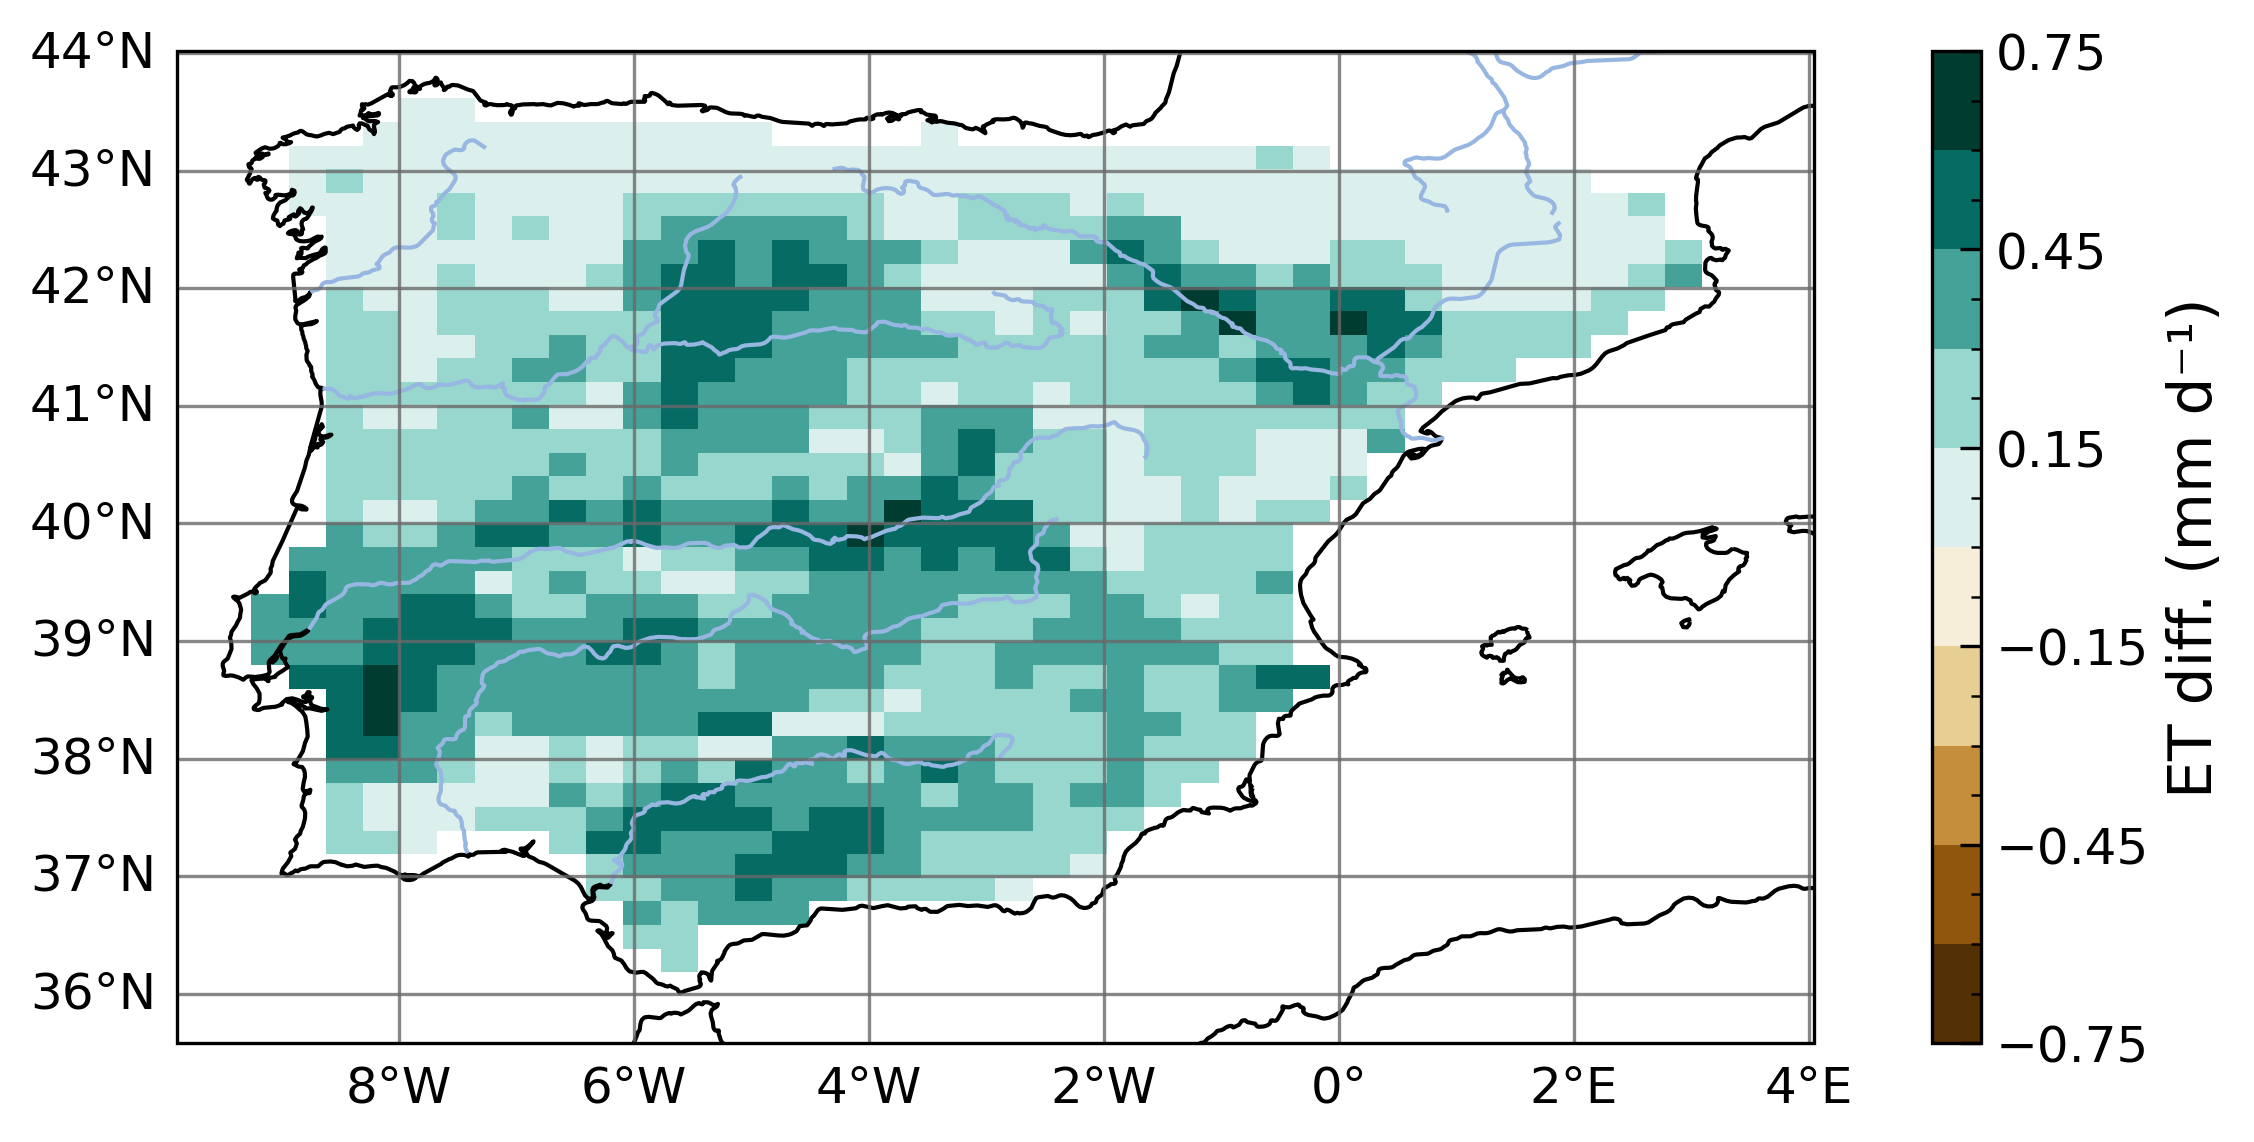
\includegraphics[width=\textwidth]{images/chap4/future/diffmap_evap_futirr.png}
        \end{subfigure} \\

        %q2m
        \begin{subfigure}[b]{0.5\textwidth}
            \caption{2-m specific humidity difference}
            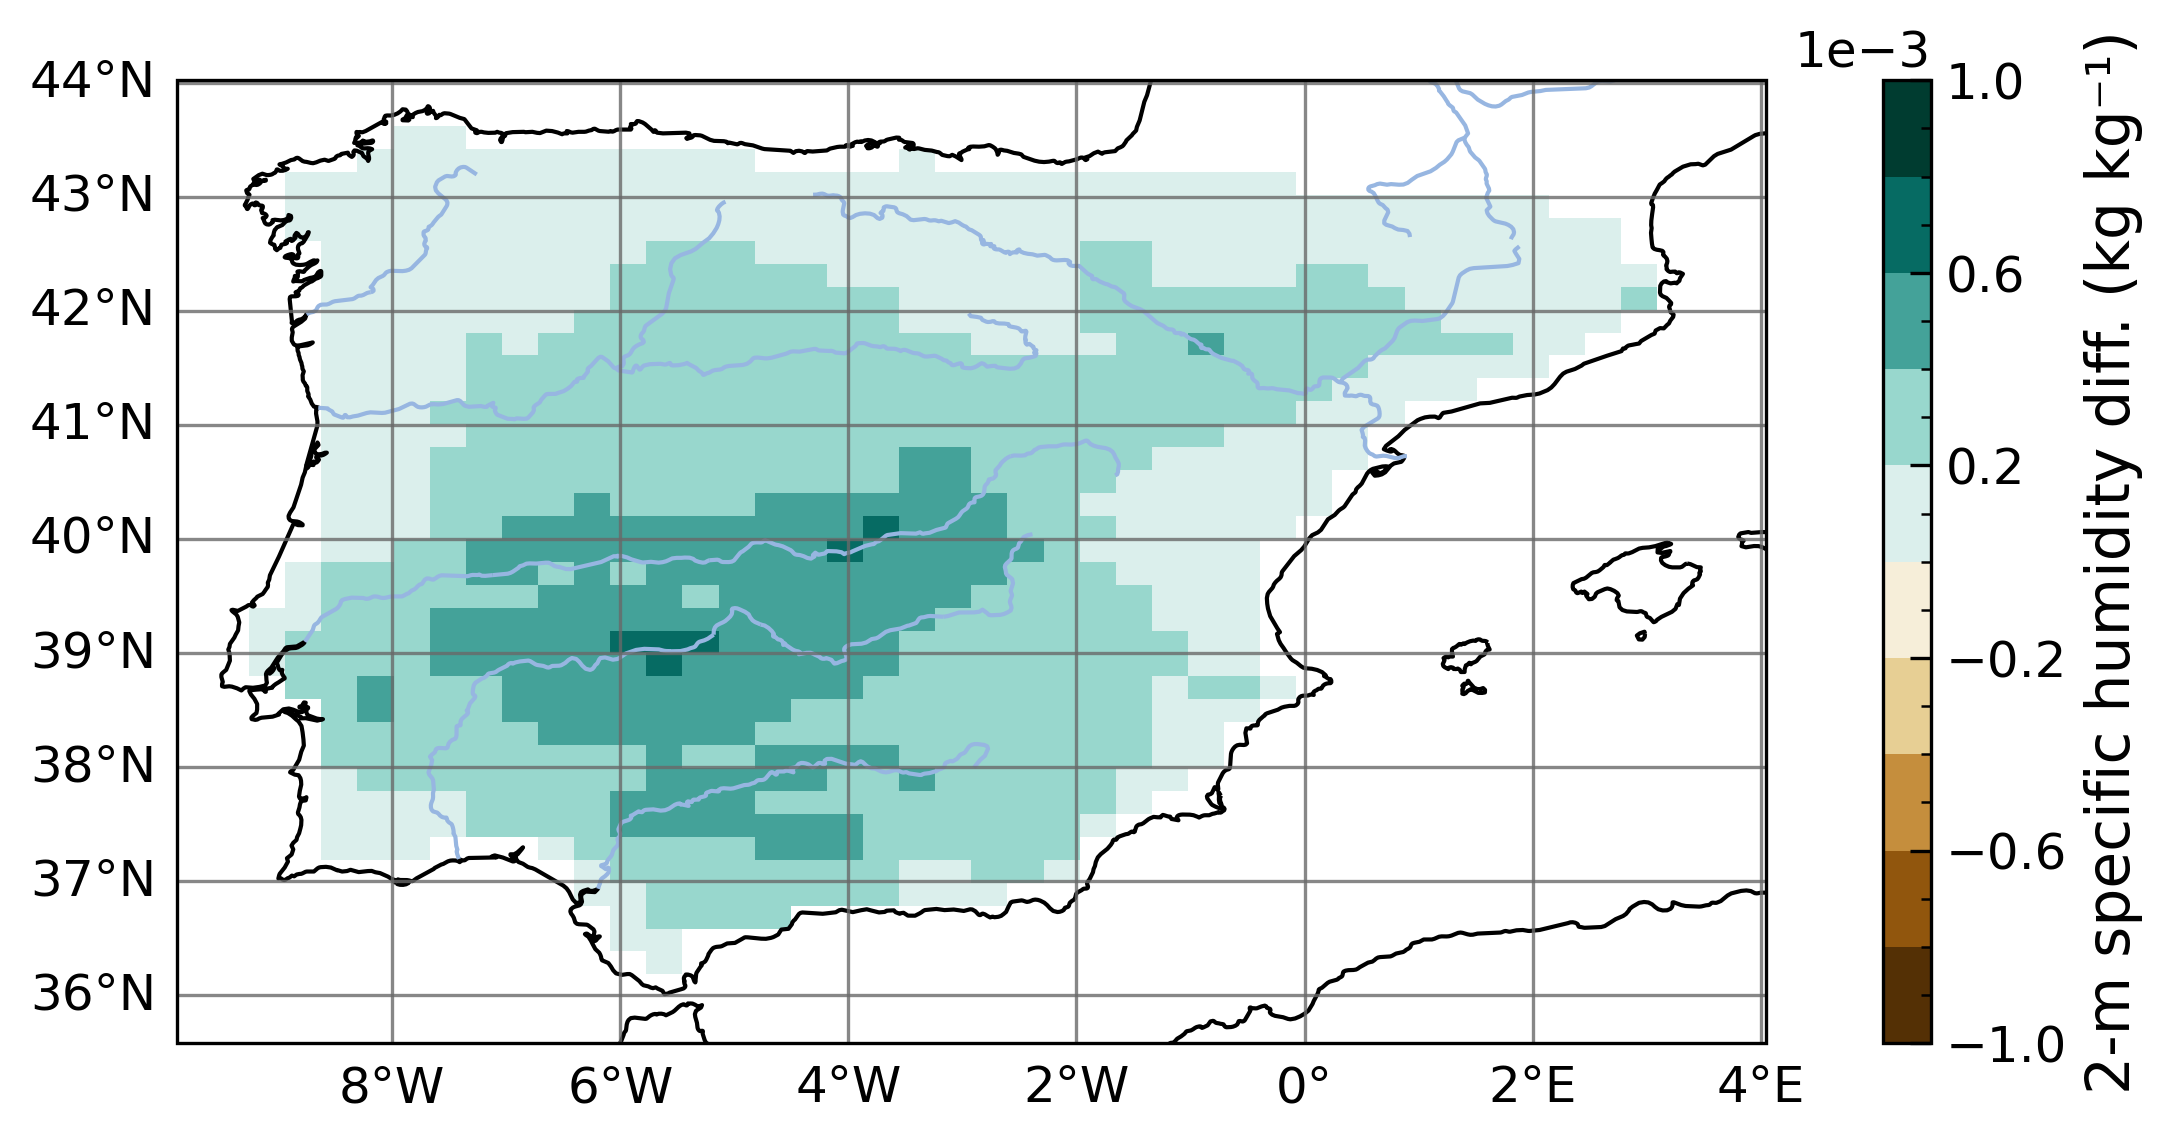
\includegraphics[width=\textwidth]{images/chap4/future/diffmap_q2m_futirr.png}
        \end{subfigure} &
        %rh2m
        \begin{subfigure}[b]{0.5\textwidth}
            \caption{2-m relative humidity difference}
            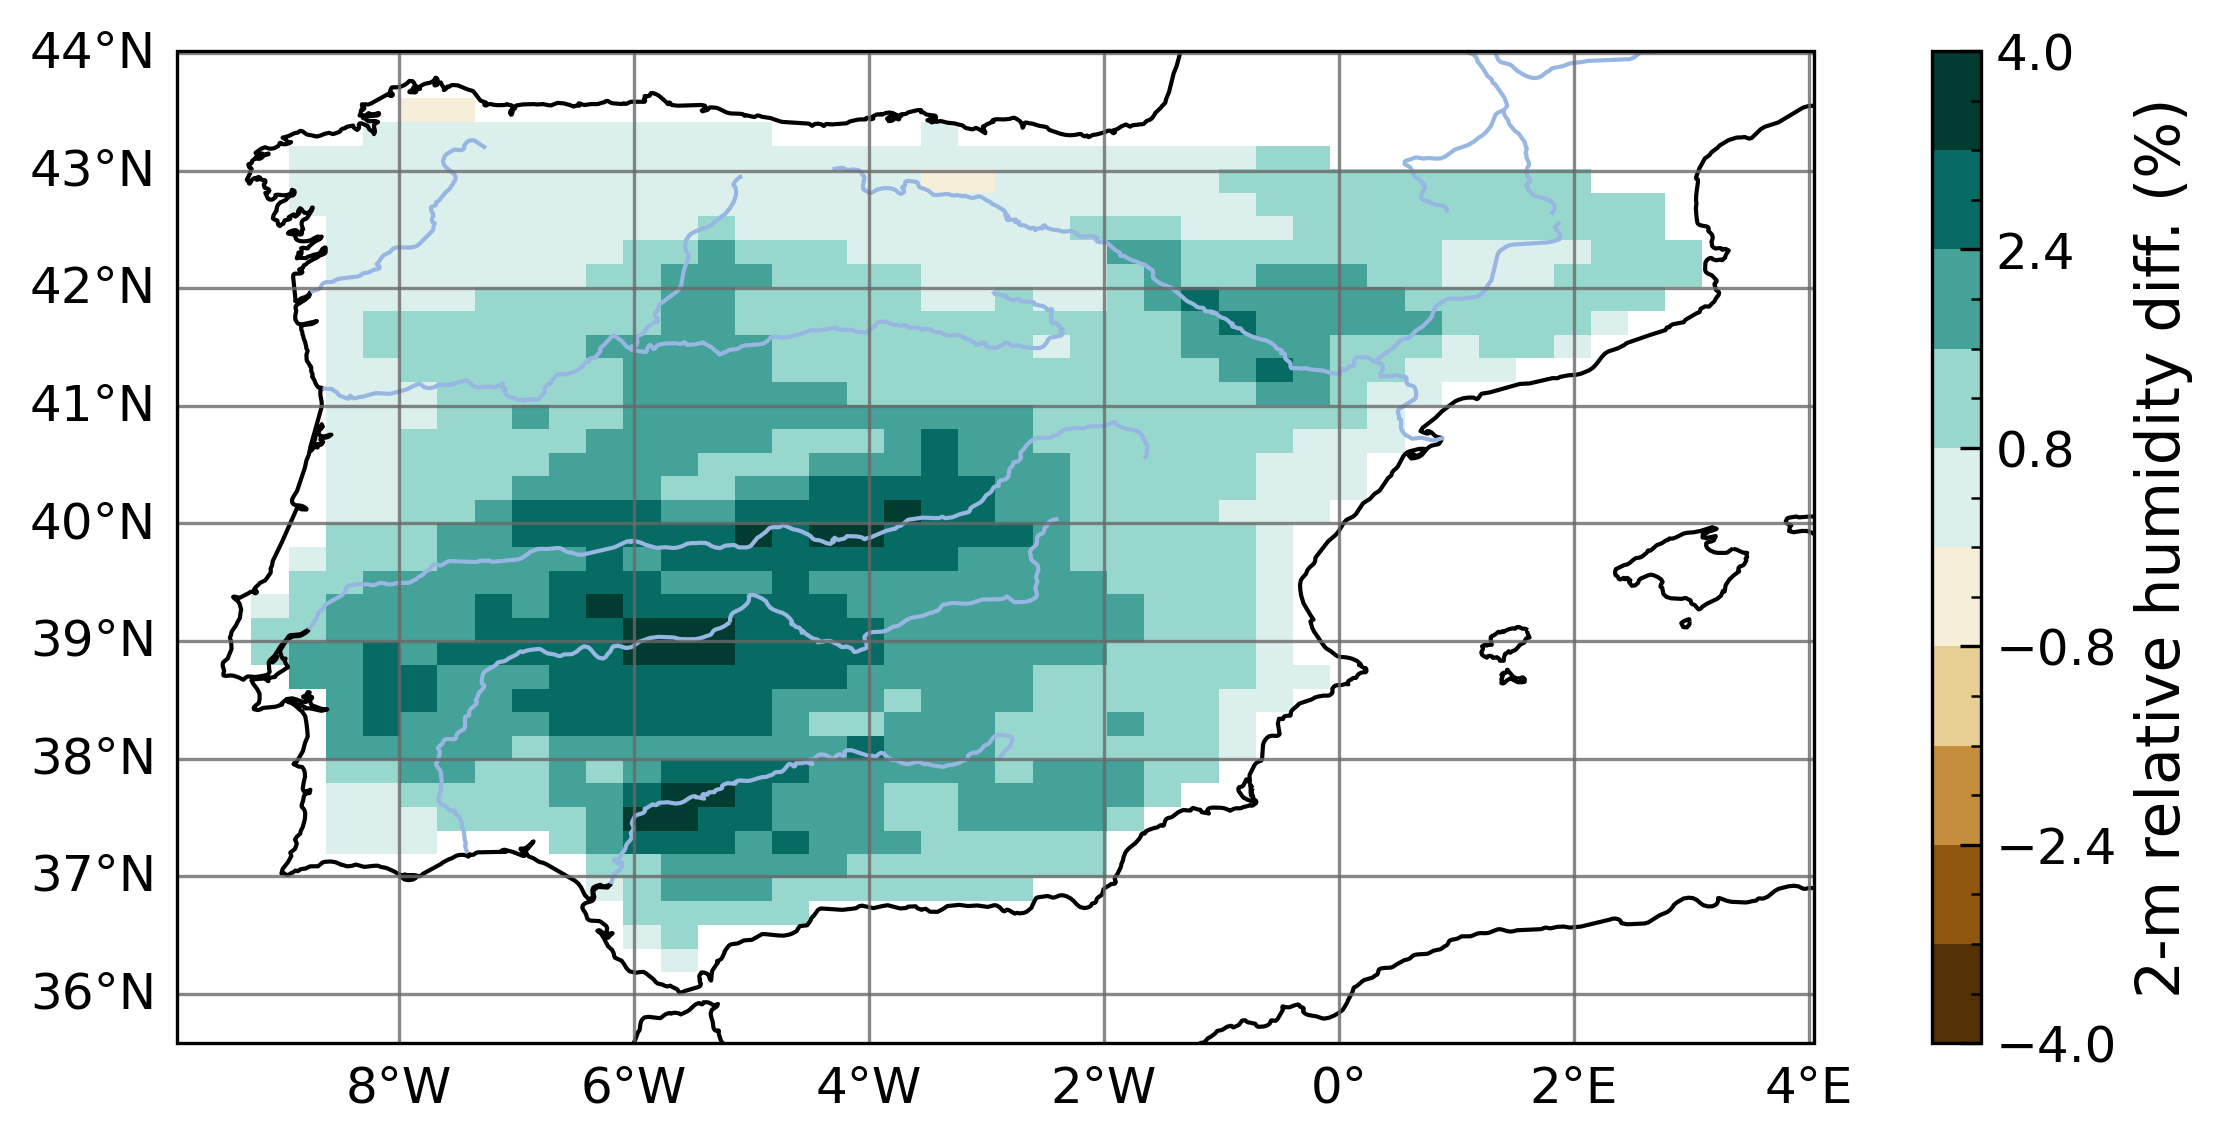
\includegraphics[width=\textwidth]{images/chap4/future/diffmap_rh2m_futirr.png}
        \end{subfigure} \\

        %pblh
        \begin{subfigure}[b]{0.5\textwidth}
            \caption{Atmospheric boundary layer height difference}
            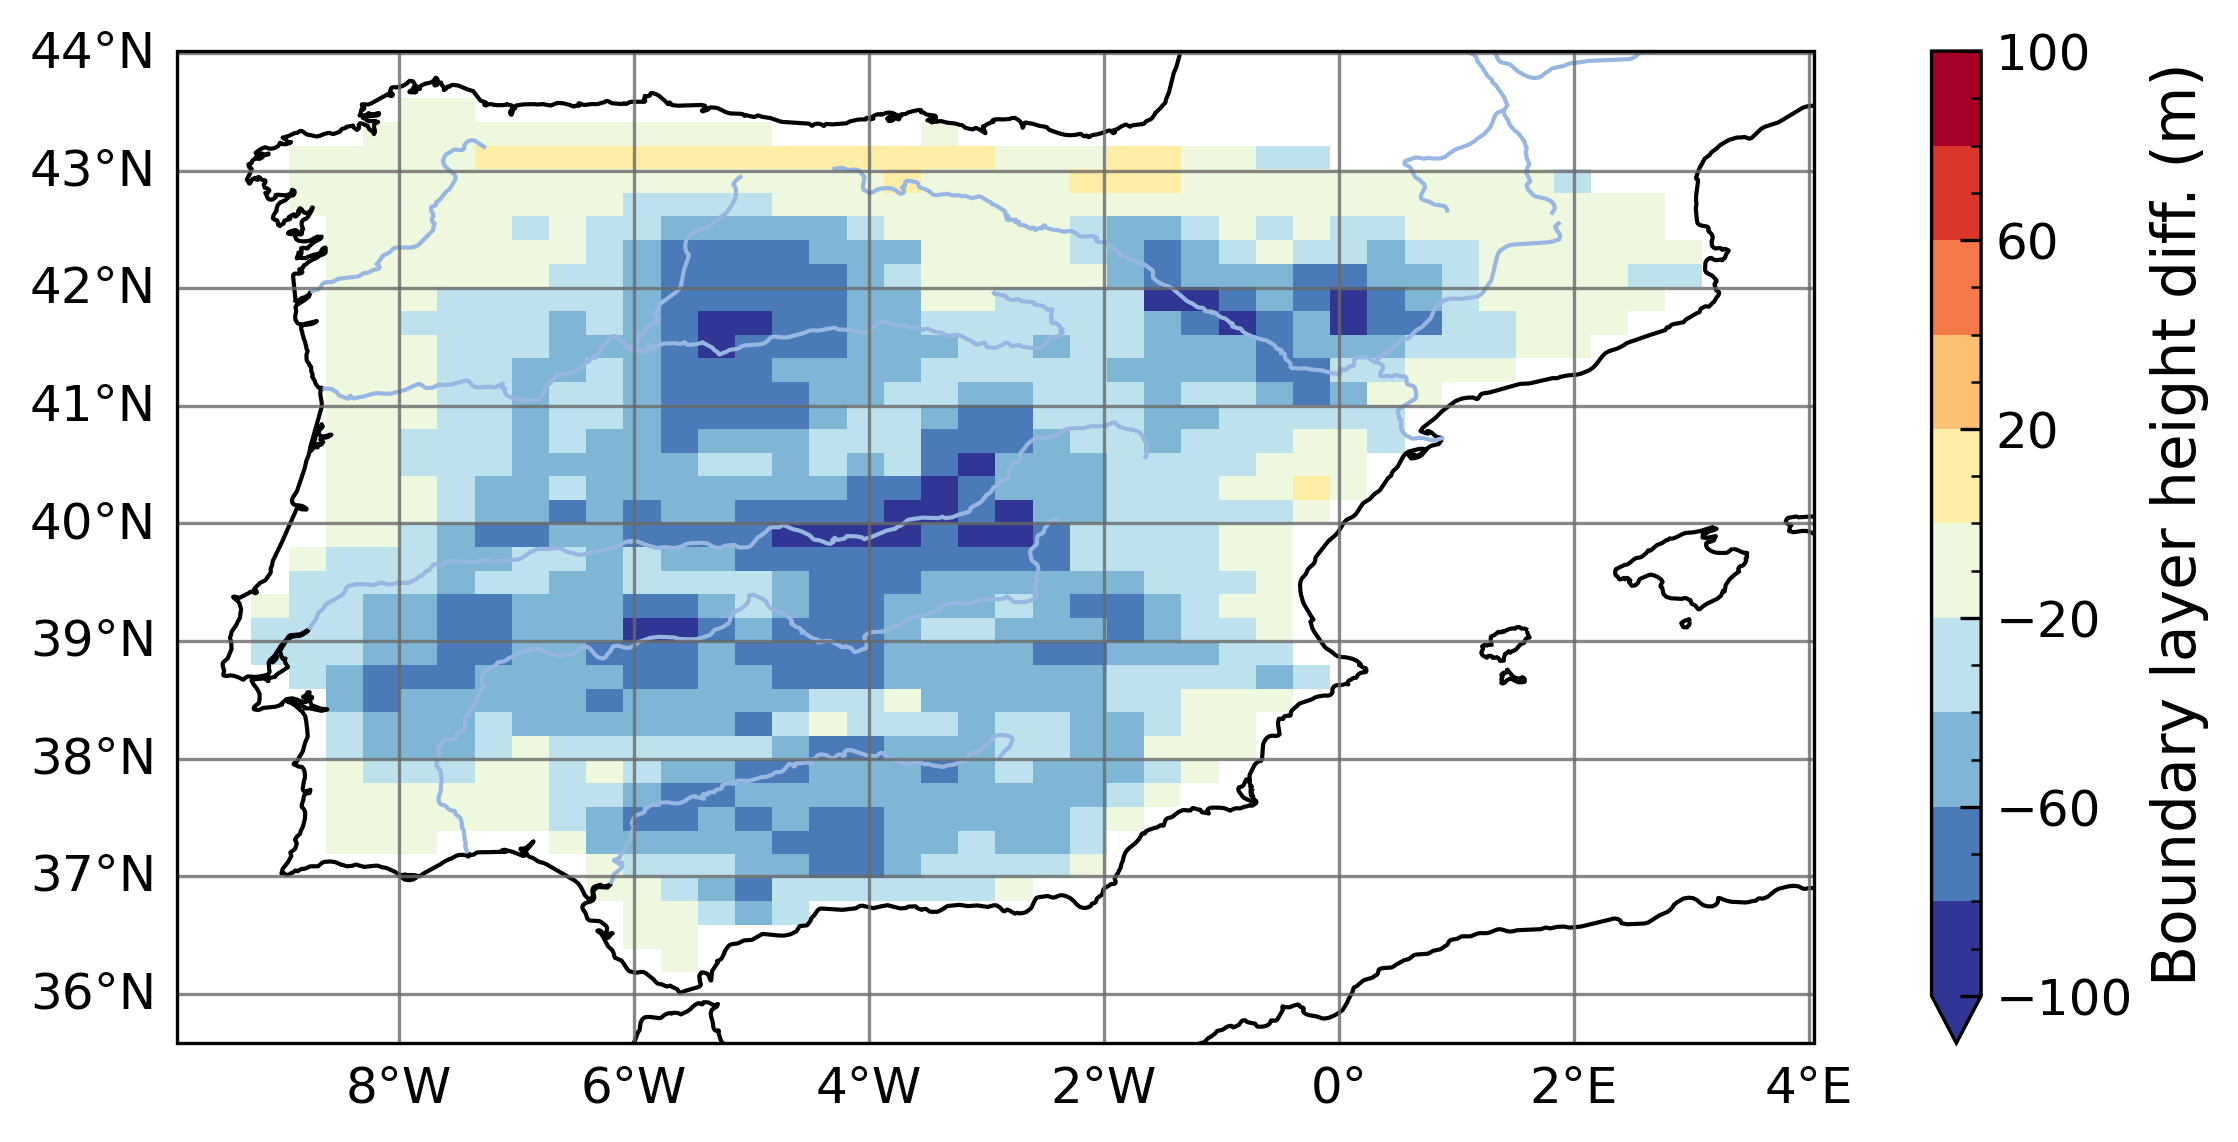
\includegraphics[width=\textwidth]{images/chap4/future/diffmap_s_pblh_futirr.png}
        \end{subfigure} &
        %lcl
        \begin{subfigure}[b]{0.5\textwidth}
            \caption{Lifting condensation level difference}
            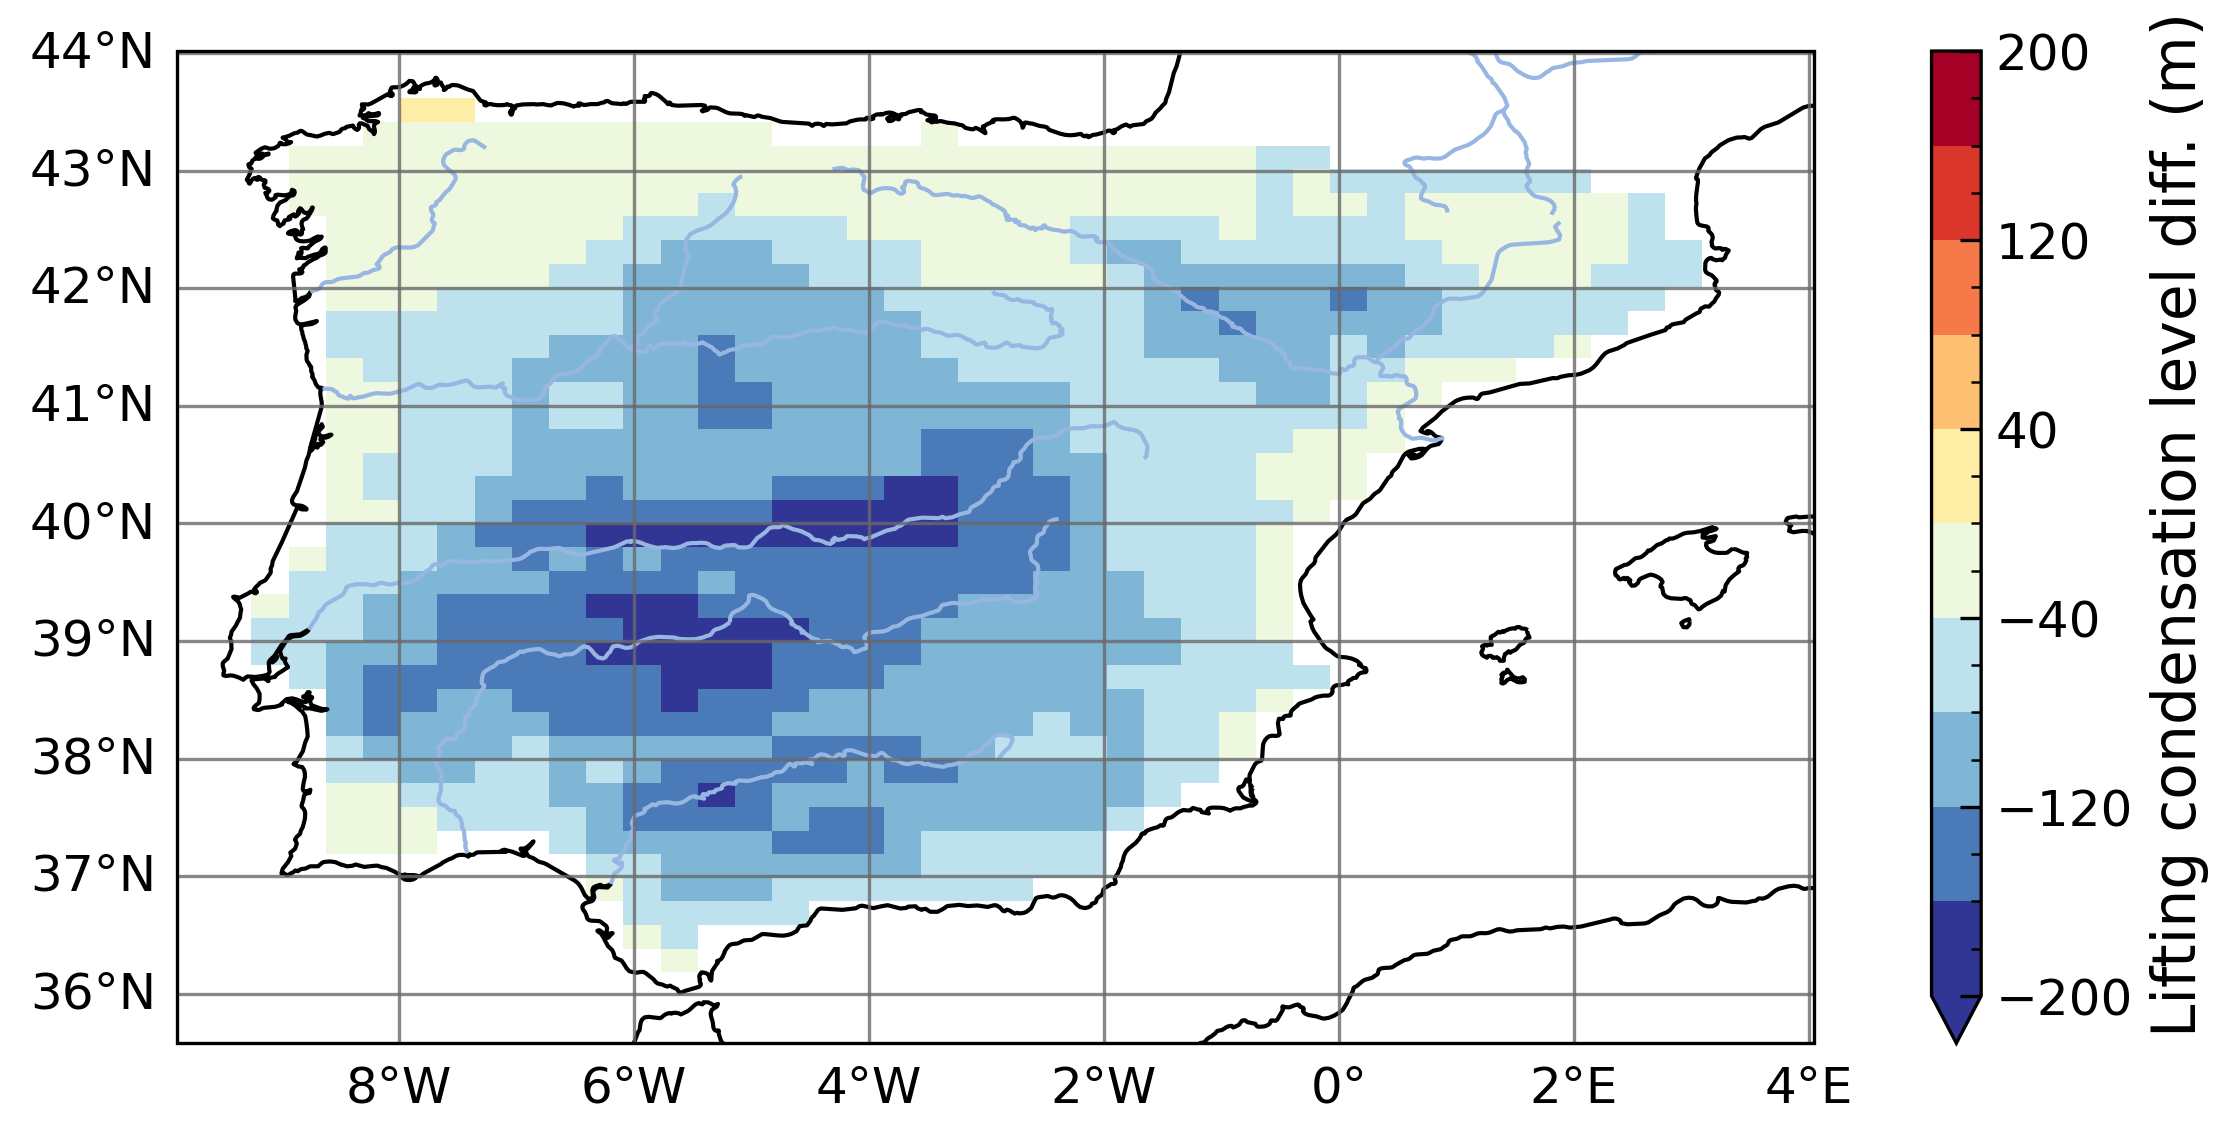
\includegraphics[width=\textwidth]{images/chap4/future/diffmap_s_lcl_futirr.png}
        \end{subfigure} \\
    \end{tabular}
    \caption{Impacts of irrigation under climate change (2050-2062). Annual mean difference between \futirr and \futnoirr.}
    \label{fig:diffmaps_future_irr}
\end{figure}

% present, no_irr : 2.18771 (mm d⁻¹)
% future, no_irr : 1.86688 (mm d⁻¹)
% future, irr : 1.89212 (mm d⁻¹)
% present, no_irr : 1.27330 (mm d⁻¹)
% future, no_irr : 1.17734 (mm d⁻¹)
% future, irr : 1.44247 (mm d⁻¹)
% present, no_irr : 14.66318 (°C)
% future, no_irr : 16.98357 (°C)
% future, irr : 16.80824 (°C)
% present, no_irr : 50.54140 (W m⁻²)
% future, no_irr : 55.53161 (W m⁻²)
% future, irr : 49.91047 (W m⁻²)
% present, no_irr : 0.00730 (kg kg⁻¹)
% future, no_irr : 0.00786 (kg kg⁻¹)
% future, irr : 0.00813 (kg kg⁻¹)
% present, no_irr : 942.46790 (m)
% future, no_irr : 946.90222 (m)
% future, irr : 909.96997 (m)
% present, no_irr : 884.01685 (m)
% future, no_irr : 1039.27222 (m)
% future, irr : 959.86011 (m)
% present, no_irr : 68.83486 (%)
% future, no_irr : 65.23708 (%)
% future, irr : 66.66062 (%)

\clearpage

\subsection{Aridification and impact of irrigation}

Aridity indices are often used as a way to characterize continental regions and how their climate will evolve in the future, under climate change. Aridity aims to describe long-term moisture deficits that limit the development of vegetation. Several definitions and indices have been proposed and used in the last decades, but the most common is the United Nations Environmental Programme (UNEP) aridity index, defined as the ratio of the annual precipitation to potential evapotranspiration : $AI = \frac{P}{PET}$. %todo:refs (Begueria 2025, UNEP 1992)
This index is most relevant when averaged over multiple years to reduce sensitivity to specific droughts or extreme precipitation events.

At the end of Mariame Maiga's internship, a short study of the evolution of aridity in ICOLMDZOR was conducted, using this index to classify grid cells into five aridity classes as presented in Table \ref{table:aridity_classes}. 
Potential evapotranspiration was taken from ORCHIDEE's \textit{evapot\_corr} variable, named $E_{pot}^*$ in the equations of Chapter \ref{chap:methods}, which is computed using the formulation of \citet{Budyko_1956} with a correction from \citet{milly_potential_1992}. 
Even though the choice of the method used to compute PET has a strong impact on the value of the aridity index and on the classification of each grid cell, this index remains an interesting tool to study the future evolution of aridity in the various regions of the Peninsula.

\begin{table}[h]
    \centering
    \begin{tabular}{|l|l|}
        \hline
        \textbf{Aridity class} & \textbf{Index values} \\
        \hline
        Hyper-arid & \( AI < 0.05 \) \\
        \hline
        Arid & \( 0.05 < AI < 0.2 \) \\
        \hline
        Semi-arid & \( 0.2 < AI < 0.5 \) \\
        \hline
        Dry sub-humid & \( 0.5 < AI < 0.65 \) \\
        \hline
        Humid & \( 0.65 < AI \) \\
        \hline
    \end{tabular}
    \caption{Aridity classes based on UNEP aridity index values.}
    \label{table:aridity_classes}
\end{table}

The spatial distribution in the \presnoirr simulation (Fig. \ref{fig:aridity_index_v2}a, b) shows a dominant semi-arid climate over the Iberian Peninsula, with a humid strip in the northern coast and the Pyrenees, and arid climate in the Ebro and Guadalquivir valleys, and other areas in the South.
Under the SSP5-8.5 climate change scenario, in \futnoirr (Fig. \ref{fig:aridity_index_v2}c, d), the share of humid grid cells falls from 16.5\% to 6.8\%, and the share of semi-arid from 58.6\% to 50.1\%, while the share or arid grid cells doubles, from 18.5\% to 36.1\%. This corresponds to a shift in each aridity class. Most humid areas change to dry sub-humid or even directly to semi-arid, leaving only the heart of the Pyrenees and of the Cantabrian mountain ranges in this aridity class. The arid areas, on the contrary, extend to encompass a large share of the Ebro, Guadiana and Guadalquivir basins, and the central part of the Tagus valley. This shift in aridity is consistent with the changes described in Fig. \ref{fig:diffmaps_present_future}, a decrease of precipitation and an increase in temperature which partly drives PET. %option:show evapot_corr evolution ? 

The influence of irrigation on this evolution under climate change remains limited (Fig. \ref{fig:aridity_index_v2}). The share of arid grid cells is lower in \futirr (29.4\%) than \futnoirr (36.1\%), which is mostly compensated by a larger share of semi-arid grid cells (55.4\% instead of 50.1\%) wheareas the share of dry sub-humid and humid cells increase by lass than one percentage point.
This impact is mostly visible in the northwestern part of the Peninsula, and in the mountain ranges on both sides of the Guadalquivir valley, the Sierra Morena (which separates it from the Guadiana basin) and the Betic System (in the South East). Irrigation has an effect on the aridity index through the moistening and cooling of the lower atmosphere, which can decrease PET, and through the changes in precipitation. As described in Fig. \ref{fig:diffmaps_future_irr}, the cooling induced by irrigation is rather small compared to the warming induced by climate change, and the increases in precipitation are mostly located in the elevated areas. This explains why irrigation is not able to limit the expansion of the arid areas in the valleys under climate change, and mostly affects aridity in the mountainous regions. This result is clearly dependent on the choice of the aridity index, but in practical terms, it points to the fact that irrigation is an adaptation strategy which can help sustaining plant growth in the valleys, but with limited long-term benefits on the local climate over cultivated areas.

%figure : maps of aridity index classes for present and future
\begin{figure}[htbp]
    \centering
    %pres, no_irr
    \begin{subfigure}[b]{0.67\textwidth}
        \caption{Aridity index classes in \presnoirr (2010-2022)}
        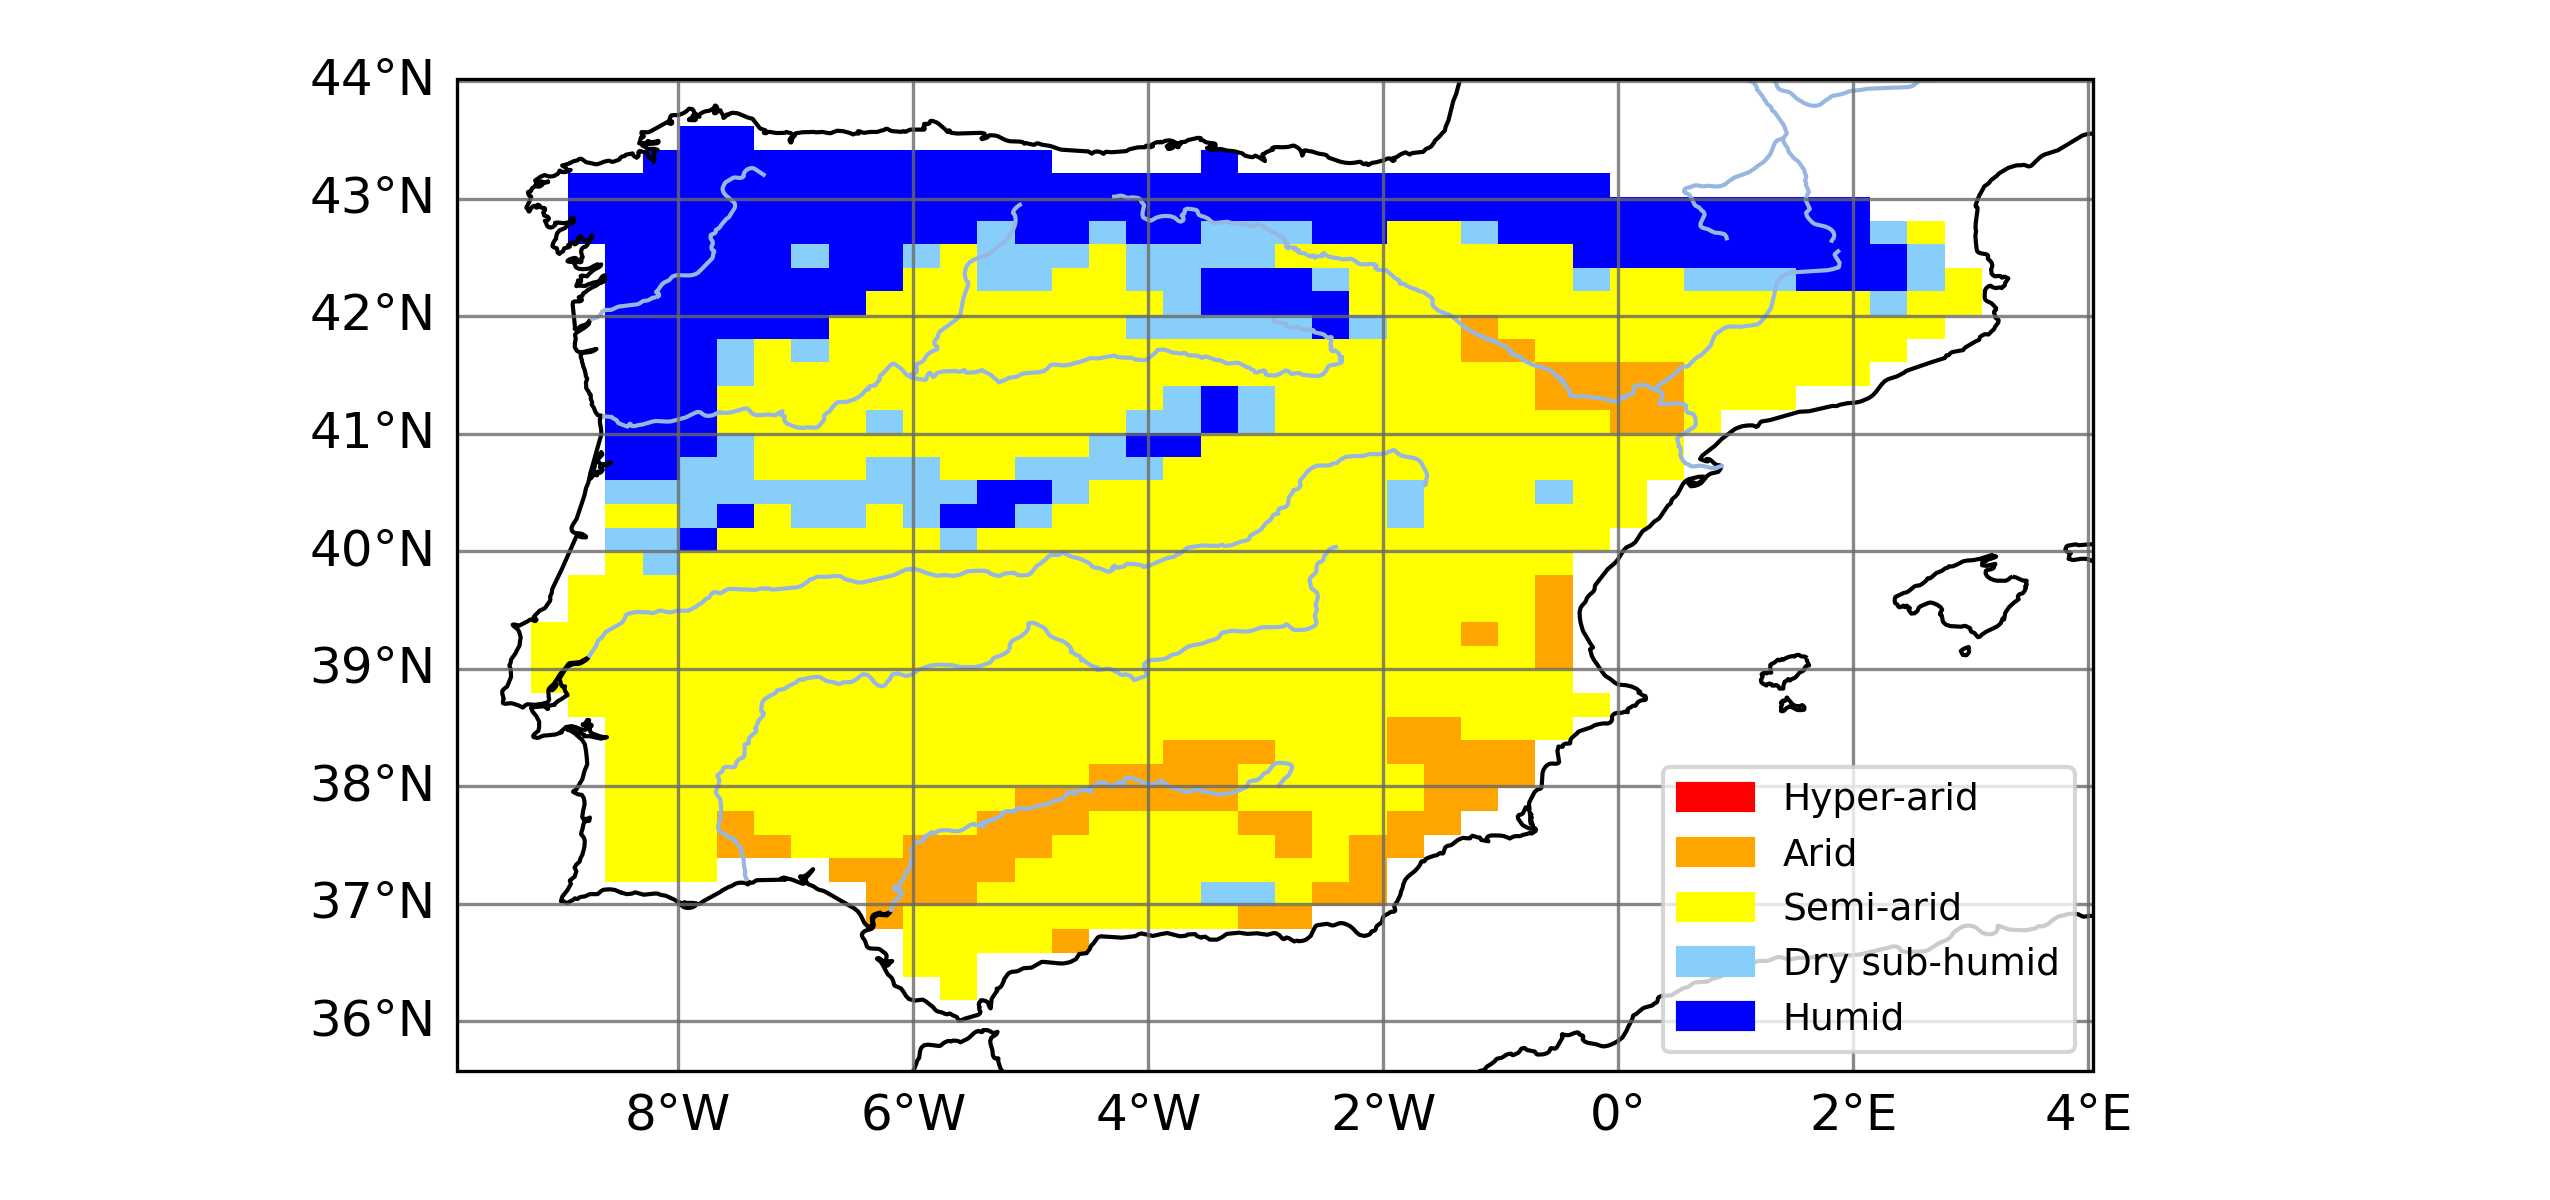
\includegraphics[width=\textwidth]{images/chap4/future/aridity_index_pres_noirr.png}
    \end{subfigure}
    \begin{subfigure}[b]{0.31\textwidth}
        \caption{Share of aridity index classes in \presnoirr (2010-2022)}
        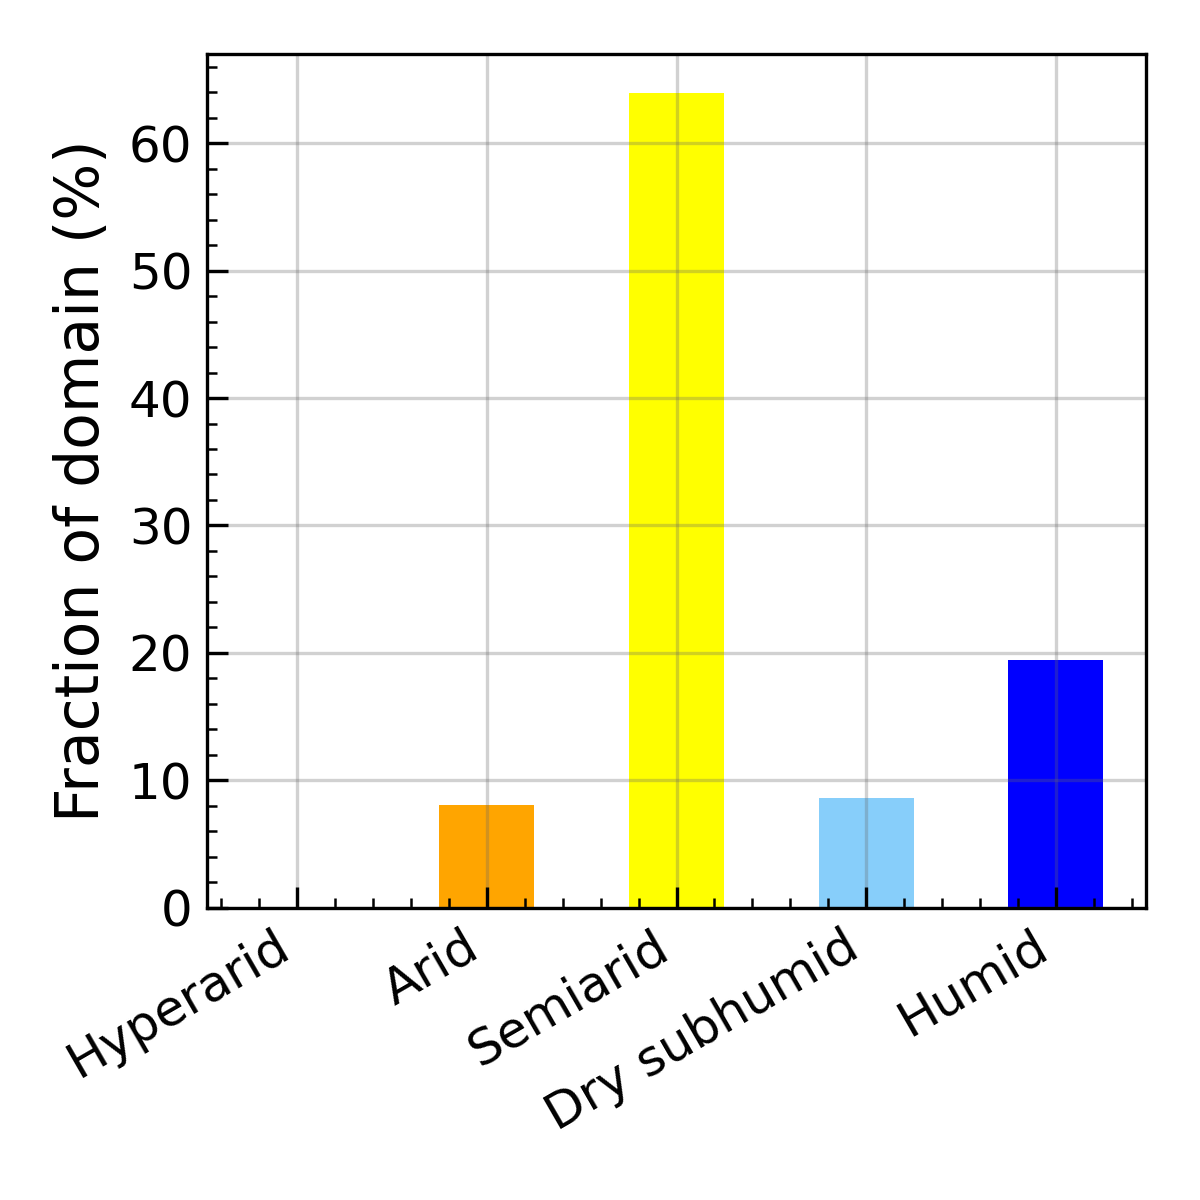
\includegraphics[width=\textwidth]{images/chap4/future/aridity_index_distribution_pres_noirr.png}
    \end{subfigure} \\

    %future, noirr
    \begin{subfigure}[b]{0.67\textwidth}
        \caption{Aridity index classes in \futnoirr (2050-2062)}
        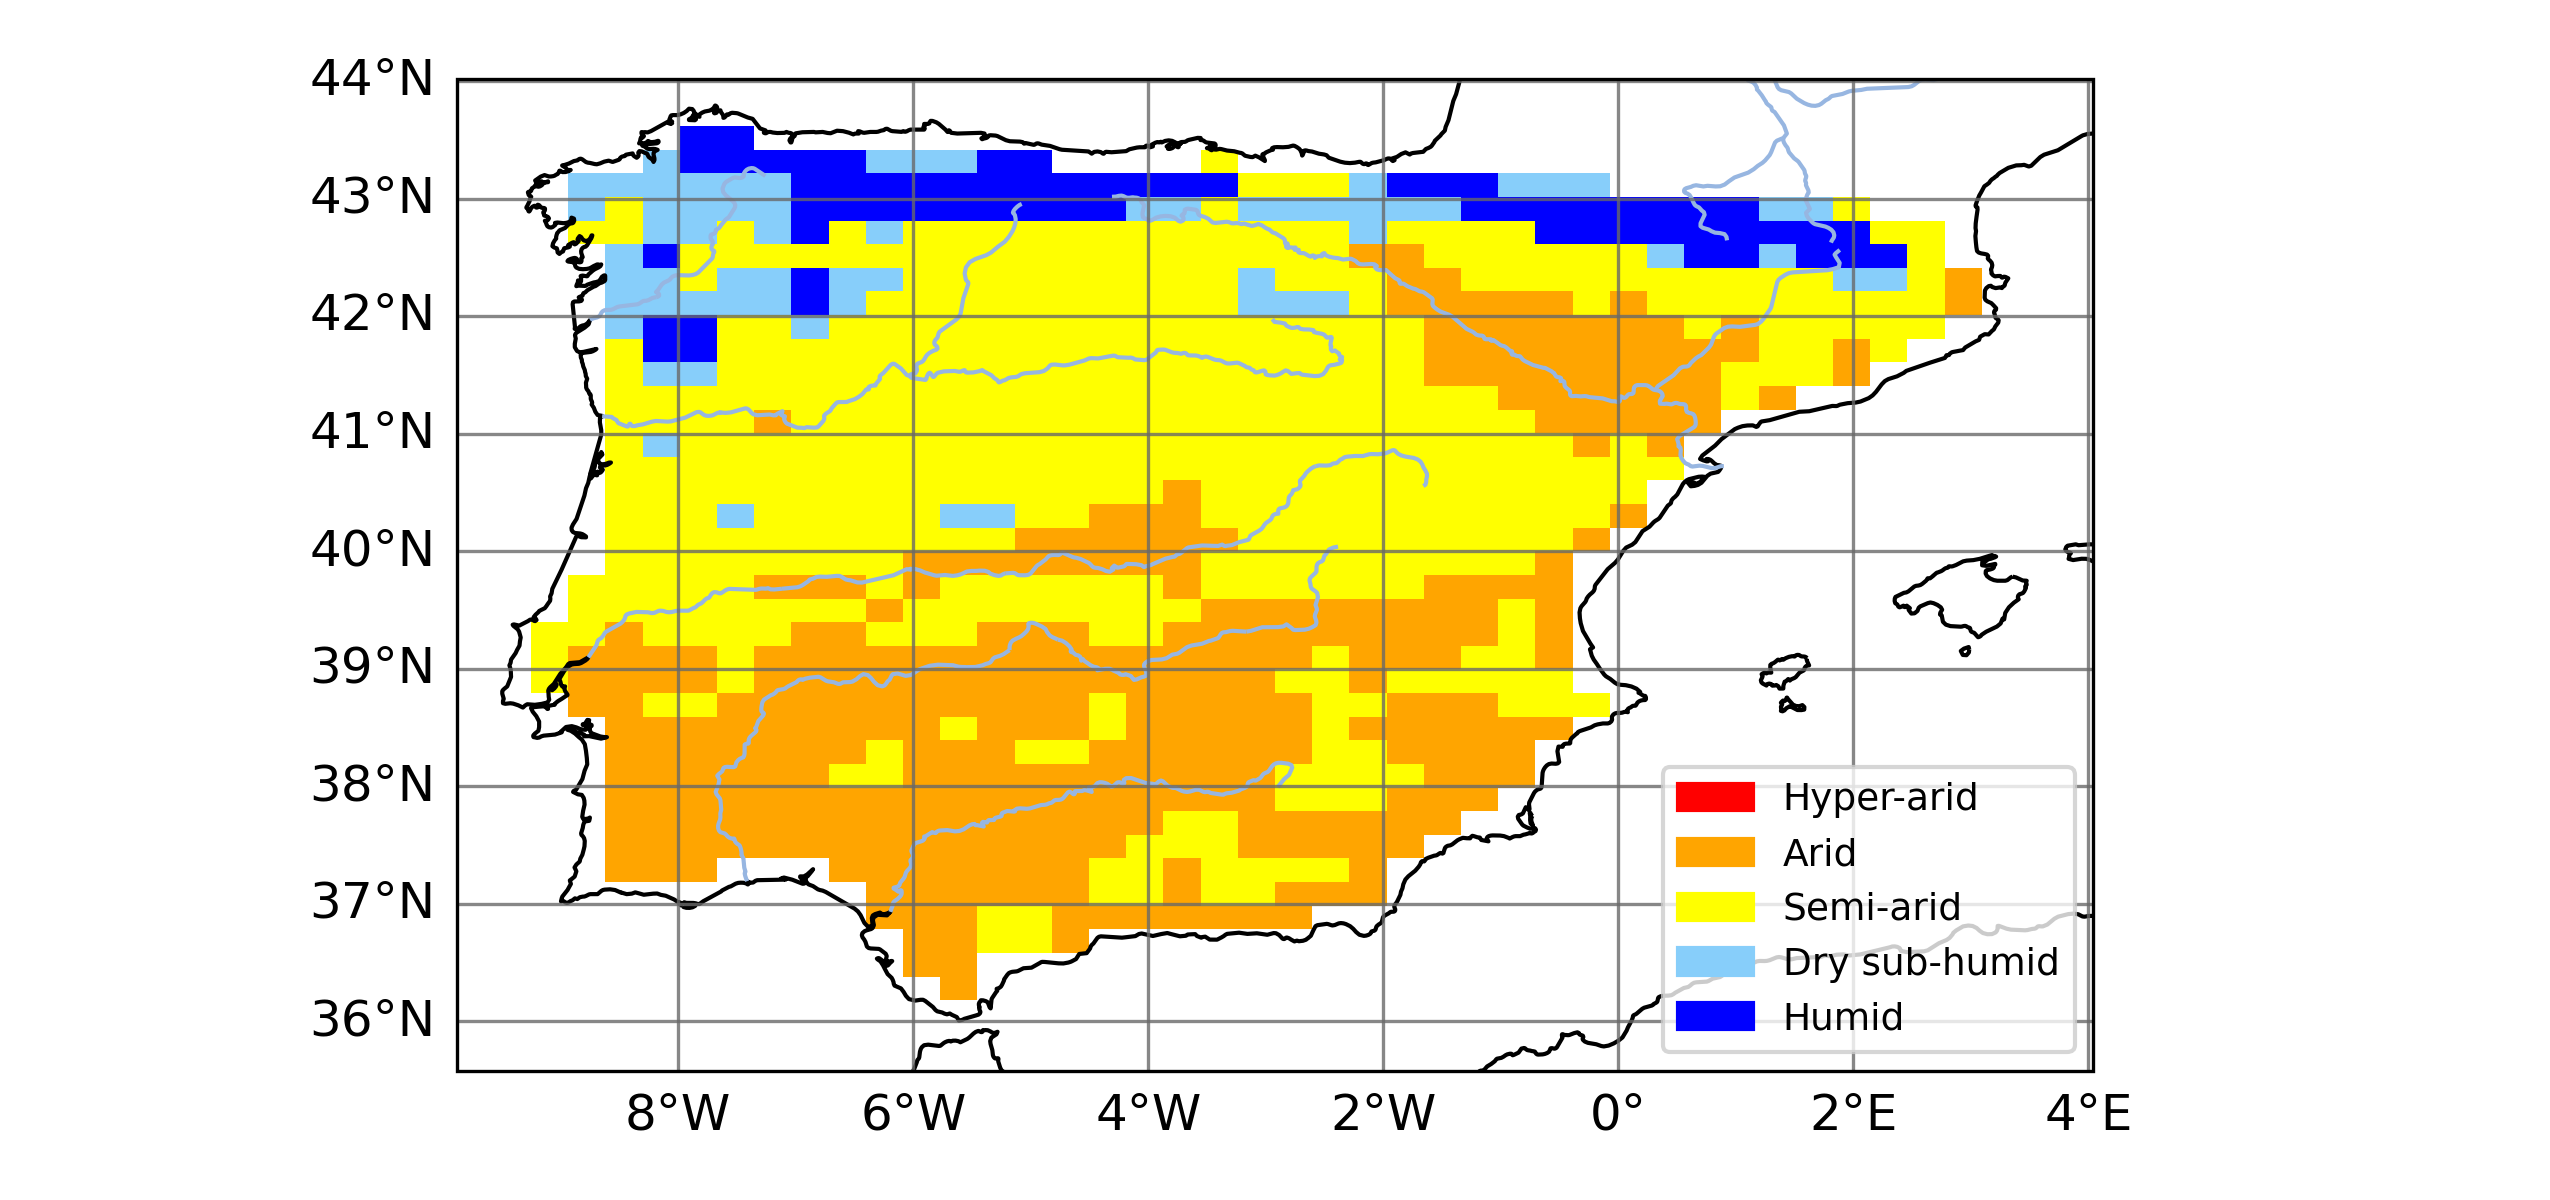
\includegraphics[width=\textwidth]{images/chap4/future/aridity_index_fut_noirr.png}
    \end{subfigure}
    \begin{subfigure}[b]{0.31\textwidth}
        \caption{Share of aridity index classes in \futnoirr (2050-2062)}
        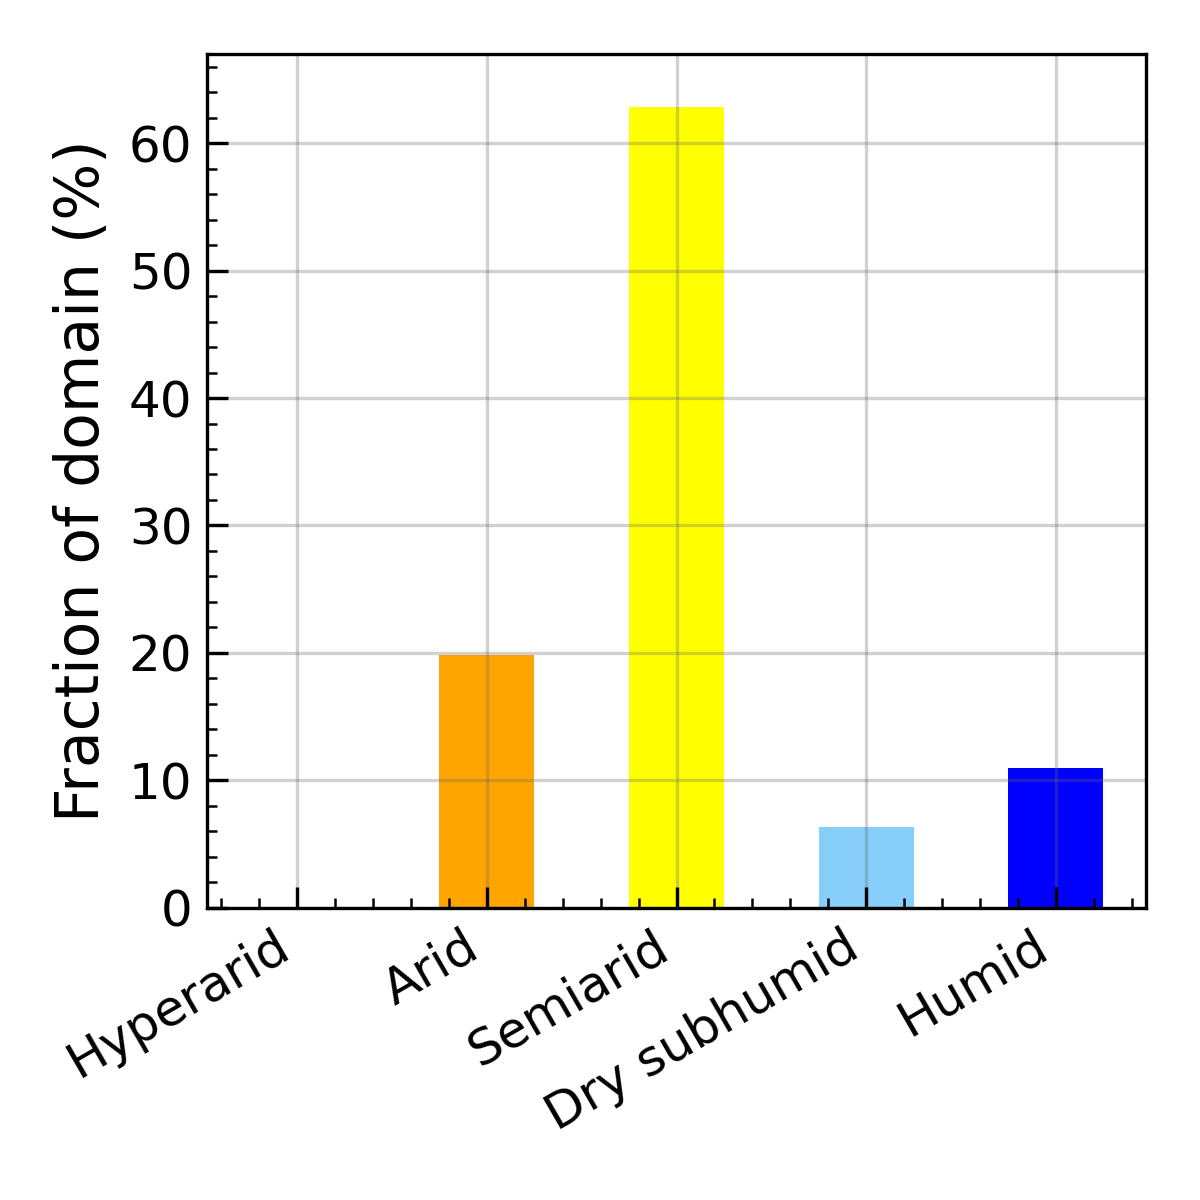
\includegraphics[width=\textwidth]{images/chap4/future/aridity_index_distribution_fut_noirr.png}
    \end{subfigure} \\

    %future, irr
    \begin{subfigure}[b]{0.67\textwidth}
        \caption{Aridity index classes in \futirr (2050-2062)}
        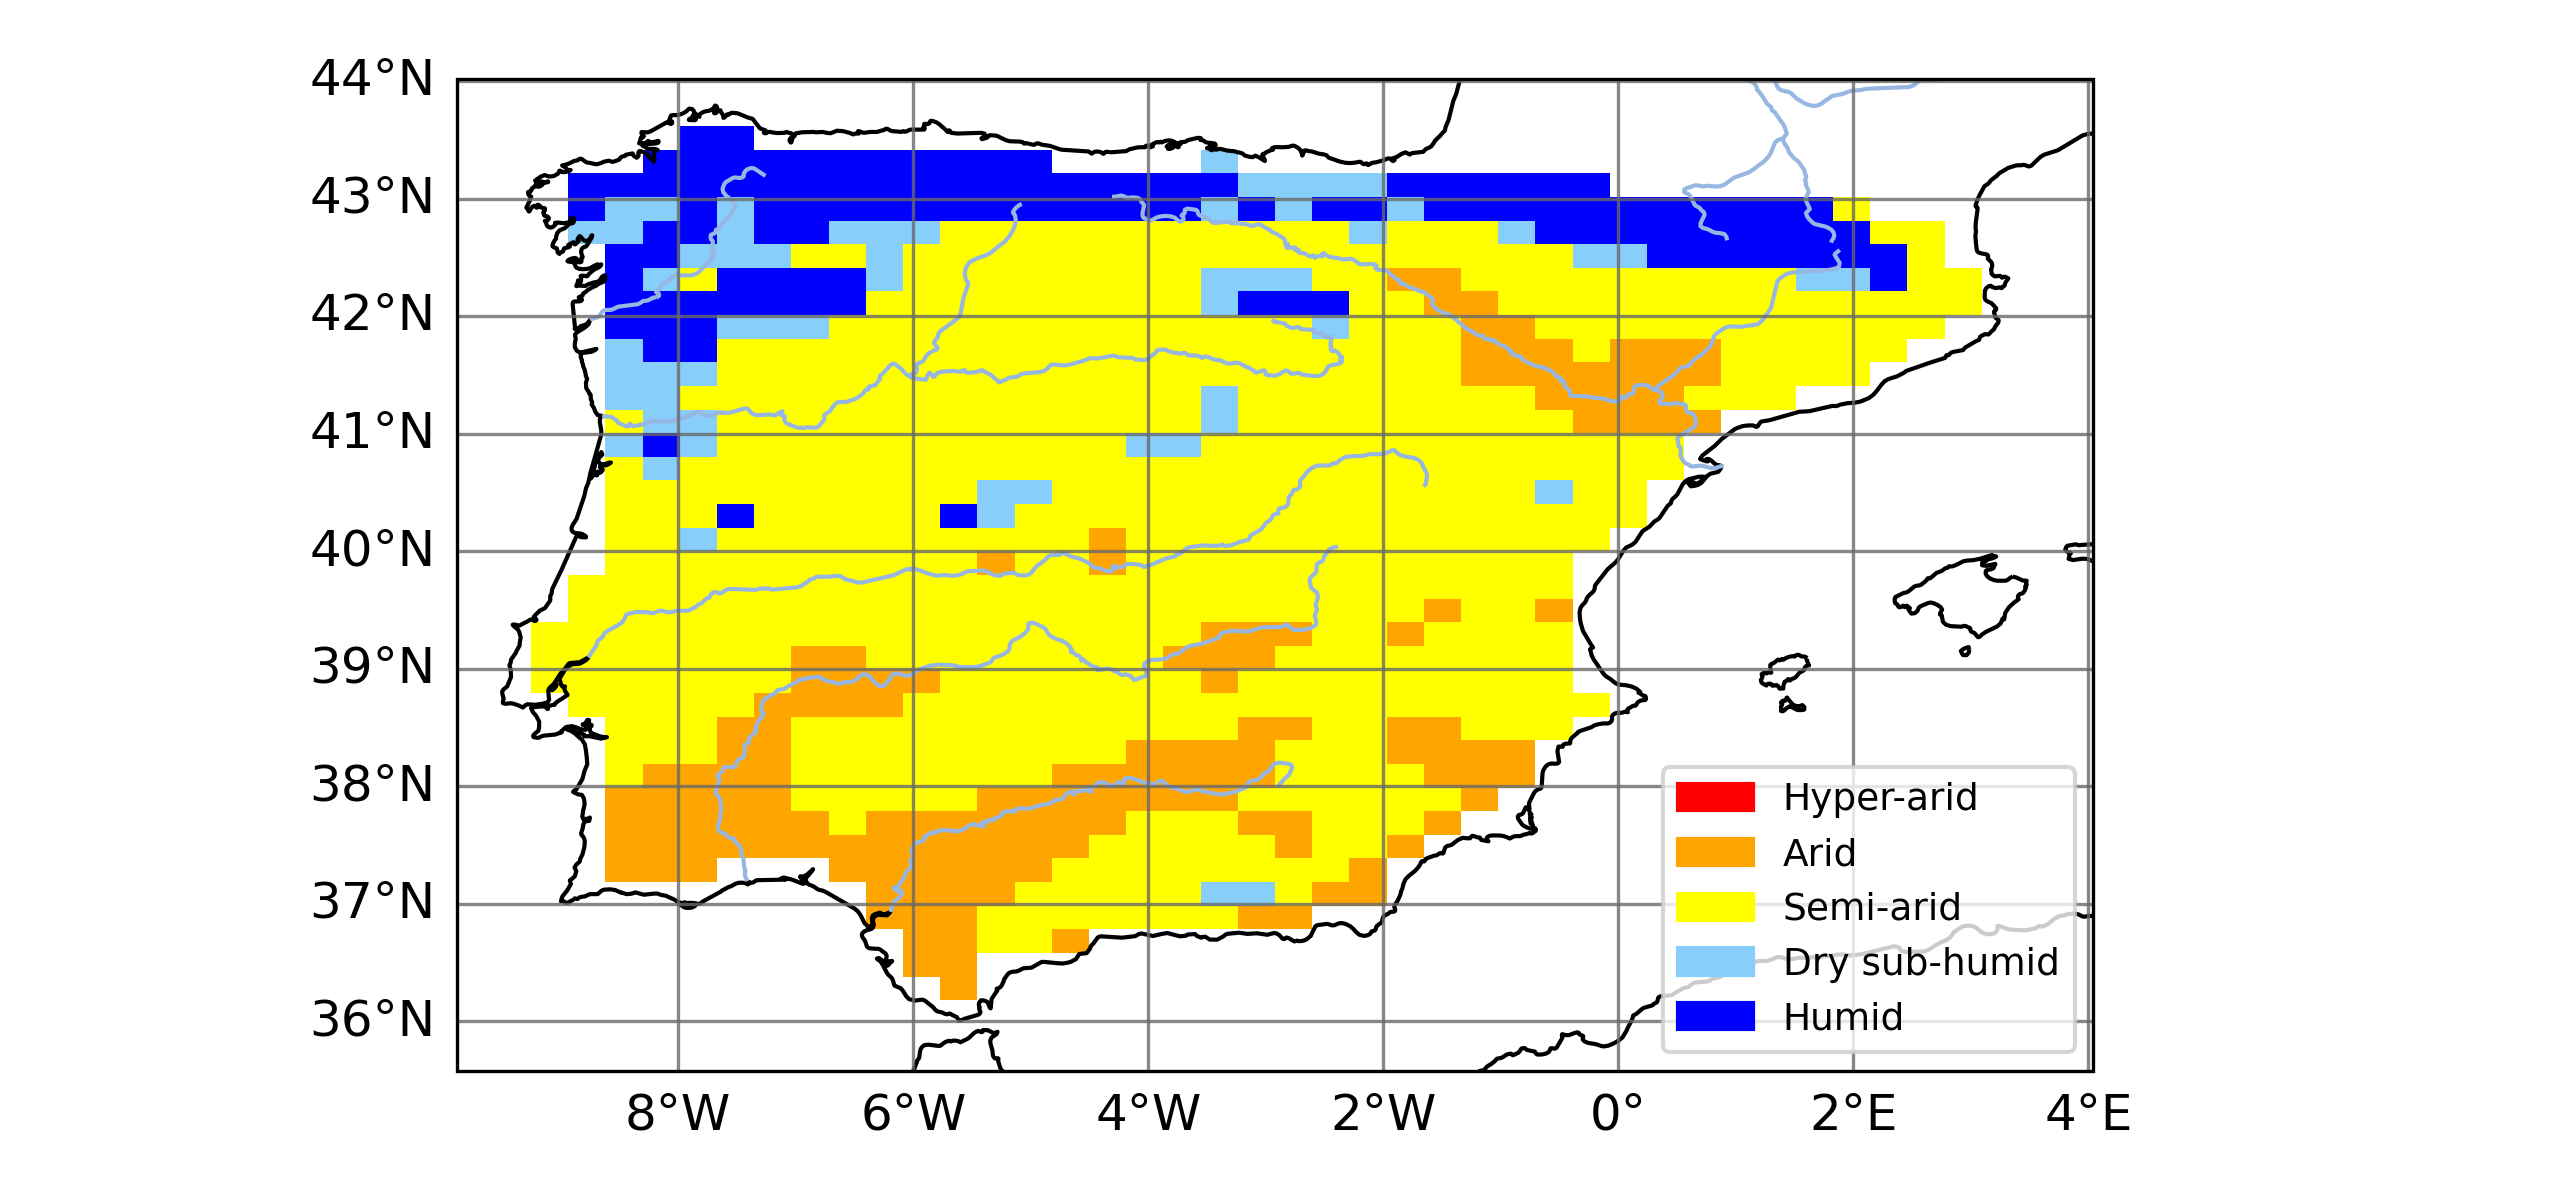
\includegraphics[width=\textwidth]{images/chap4/future/aridity_index_fut_irr.png}
    \end{subfigure}
    \begin{subfigure}[b]{0.31\textwidth}
        \caption{Share of aridity index classes in \futirr (2050-2062)}
        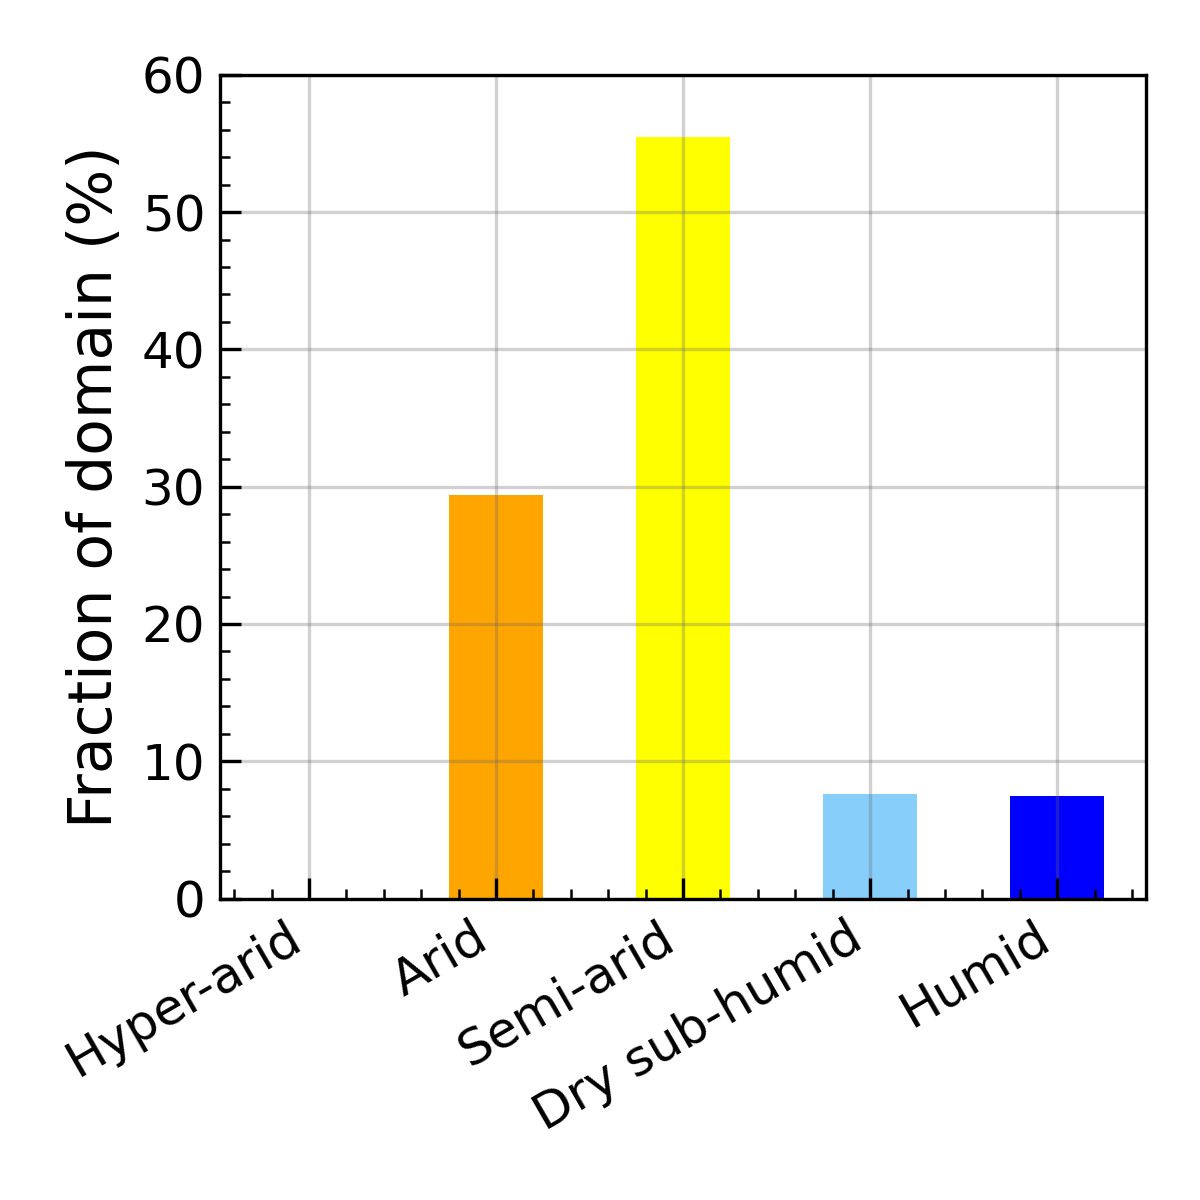
\includegraphics[width=\textwidth]{images/chap4/future/aridity_index_distribution_fut_irr.png}
    \end{subfigure}
    \caption{Spatial distribution of aridity index classes in the \presnoirr, \futnoirr, and \futirr simulations.}
    \label{fig:aridity_index_v2}
\end{figure}

%pres_no_irr
% Arid: 171 grid cells (18.566775244299674)
% semi-arid: 540 grid cells (58.63192182410424)
% Dry sub-humid: 58 grid cells (6.297502714440825)
% Humid: 152 grid cells (16.503800217155266)

%fut_no_irr
% Arid: 333 grid cells (36.156351791530945)
% semi-arid: 462 grid cells (50.1628664495114)
% Dry sub-humid: 63 grid cells (6.840390879478828)
% Humid: 63 grid cells (6.840390879478828)

%fut_irr
% Arid: 271 grid cells (29.42453854505972)
% semi-arid: 511 grid cells (55.48317046688383)
% Dry sub-humid: 70 grid cells (7.600434310532031)
% Humid: 69 grid cells (7.491856677524431)

\clearpage

\section{Chapter conclusions}

This chapter presents results from coupled simulations with the ICOLMDZOR LAM to study the regional climate of the Iberian Peninsula, and the impacts irrigation has on this climate and the water cycle, through land-atmosphere interactions. 

\hfill

The impacts of irrigation on land surface-atmosphere coupling variables and the water cycle over the Iberian Peninsula were first studied in the present climate. Two simulations were run, with and without irrigation, using hourly ERA5 forcing data, which was the only option technically available at the time. A larger domain size than initially envisionned was selected (the intermediate domain size), to limit the impact of the transition zone discrepancies on the study area.

This study first showed that the ORCHIDEE irrigation scheme simulates realistic values from April to September in areas where surface water withdrawals are most important, such as the Ebro Valley. However, it cannot represent winter irrigation, or satisfy irrigation demand in southern regions, where actual irrigation is more dependent on groundwater pumping and river dams, due to low available volumes in rivers and groundwater routing reservoirs. Ongoing developments to add river dams into the ORCHIDEE routing scheme \citep{baratgin_modeling_2024} could very likely improve this aspect by representing interseasonal water storage, making more water available in summer.
Explicit dam representation could also limit the winter and spring overestimates of river discharge in anthropized areas, since water would be stored in the dam reservoirs during this season instead of flowing in the rivers. 
Overall, the irrigation parameterization reduces river discharge and enables better agreement with observations, but since it is only active when the LAI is above a defined threshold, these impacts are mostly visible in summer and autumn. Future work with a looser activation threshold for irrigation could help to represent winter crop irrigation, although it is not expected to have as significant an impact on discharge as an explicit dam representation since simulated irrigation demand would still remain low in winter. Nevertheless, precipitation biases are very likely to remain a major driver of discharge biases, largely independent of irrigation or dam representation.

The simulation of precipitation and ET over the Iberian Peninsula is satisfactory in winter and spring, but this study highlighted a large underestimation in summer and contrasted spatial patterns with positive precipitation biases in elevated regions and negative biases in plains. ET underestimation is partly improved by simulated irrigation, but remains present on average and over most of the domain. 
It was only a hypothesis at the time, but it is now clear that running simulations with ICOLMZOR output as forcing data would improve the underestimation of summer precipitation and ET, but also degrade the performance in winter river discharge due to excessive precipitation in moutainous areas.
% These linked biases might be improved with a different simulation setup, particularly in the lateral forcing. Preliminary analyses (not shown) revealed an abnormal behaviour of the model in the transition zone between the ERA5 forcing zone and the central free zone, which was attributed to discrepancies between the physics used in the model and in the reanalysis. This resulted in precipitation underestimations throughout the entire simulation domain, which were largely improved by using a larger domain for the simulations presented here. A good lead for future works would be to use lateral forcing from global simulations of the ICOLMDZOR model or nested LAM simulations rather than a reanalysis, but these options are not yet technically available.
To improve these biases would likely require more work in ICOLMDZOR, regarding the modelling of radiative processes, shallow and deep convection (whose tuning often focuses on tropical regions), or surface processes (roughness, albedo, components of ET). This highlighted the fact that the results of this study are necessarily limited by the modelling choices, uncertainties, and biases of the IPSL-CM, and therefore remain largely model-specific.

The atmospheric impacts of irrigation were analysed in detail in summer, since it is the season with the largest irrigation values and the most significant response for all variables of interest, although it is the driest season, with very little precipitation. 
In JJA, the strong response of turbulent fluxes to irrigation leads to cooling and moistening of the lower atmosphere and significantly affects its structure (LCL and ABL height), with stronger effects on intensely irrigated regions, which is consistent with the findings of \citet{rappin_landatmosphere_2022}. In contrast, significant increases in precipitation are mostly detected in lightly irrigated mountainous areas surrounding the highly irrigated Ebro Valley. This points to a dominant effect of ABL stabilization, described by \citet{findell_atmospheric_2003-1, ek_influence_2004}, in intensely irrigated areas, and remote effects of atmospheric moistening as in \citet{deangelis_evidence_2010, lo_irrigation_2013, yang_impact_2017}. 
An improved representation of winter and spring irrigation could either allow to generalize the following results or to identify different responses to irrigation under moister atmospheric conditions.
Furthermore, over the Iberian Peninsula, increases in ET are proportional to applied irrigation and actually exceed it for almost every simulation month. This is made possible by small but systematic increases in average precipitation over the domain, forming evidence of continental moisture recycling over the Iberian Peninsula. The precipitation increases are of lower magnitude than those of ET and occur much more in lightly irrigated regions than in intensely irrigated regions, confirming that the recycling is partial and mostly nonlocal.

These findings called for an analysis of surface-atmosphere coupling processes in the presence of irrigation at the diurnal scale to better describe the impacts on the ABL structure in both irrigated areas and neighbouring regions.
Therefore, the LAM was compared to field observations from the LIAISE campaign, held in the Ebro Valley in July 2021 \citep{boone_land_2025}, and to mesoscale simulations which had already been run over the campaign area and analysed in \citet{lunel_irrigation_2024,lunel_marinada_2024}. These results are presented in Chapter \ref{chap:liaise}.
%High resolution modelling experiments using irrigation parameterizations have shown large improvements of performance relative to LIAISE observations for turbulent fluxes, air temperature and humidity \citep{lunel_irrigation_2024, udina_irrigation_2024}; stressed the importance of the convection parameterization for the response of precipitation to irrigation \citep{udina_irrigation_2024}; and identified interactions of irrigation-induced heterogeneities with regional breeze circulations \citep{lunel_marinada_2024}. Conducting similar analyses with the simulation setup used in this study should provide insights into the ability of an ESM to reproduce the complex structure of these heterogeneities \citep{mangan_surface-boundary_2023} and their impacts on the ABL and atmospheric water cycle. 


\hfill

Following this study of regional climate under present conditions, another experiment was set up to study future climate conditions over the Iberian Peninsula, in the context of Mariame Maiga's internship.
Hourly lateral boundary conditions for the LAM are obtained from a global ICOLMDZOR simulation under SSP5-8.5 climate change scenario. 
One simulation was run for the present period (2010-2022), without irrigation, and two for the future period (2050-2062), with and without irrigation. This allowed for an analysis of the impacts of climate change on the region, and of the behaviour and impact of irrigation in the future. 
Although some new simulations are needed (and ongoing) to strengthen the preliminary results presented in Section \ref{sec:climate_change}, several conclusions were drawn from this study. 

Under SSP5-8.5, mid-century simulated climate is 2.3°C warmer than present climate on average over the Iberian Peninsula. Although specific humidity increases due to the water-holding capacity of the air, relative humidity decreases over all the domain, particularly in the northern mountain ranges. Cloud cover and precipitation decrease over most of the domain, with the exception of a coastal region in the Southeast, leading to a decrease in latent heat flux and an increase in sensible heat flux. Using the UNEP aridity index, a clear shift in the aridity was identified over the Peninsula, with humid regions in the North evolving towards a semiarid climate, and the arid areas in the valleys extending to cover large share of the Ebro, Guadian and Guadalquivir basins.

The simulation of future climate with irrigation showed that irrigation can counteract the effect of climate change on evapotranspiration, whereas its cooling effect is much weaker than the warming induced by climate change. Irrigation is not associated with large changes in precipitation, and the only significant increases occur in mountainous humid regions, where land-atmosphere interactions are not very impacted by additional moisture. Therefore, the impact of irrigation on the aridification of the Peninsula induced by climate change remains limited to a few grid cells.

This work on climate change and the impact of irrigation in the future, conducted in the context of a Masters student's internship, remains preliminary and calls for further investigation. Longer simulations are currently being run over 30-year periods to strengthen the statistical significance of the results. They will also include a simulation of present climate with irrigation, run with the same setup as the other three simulations, to enable a relevant comparison of irrigation demand and irrigated volumes in the two periods.

\clearpage
